% Load the kaobook class
\documentclass[
	fontsize=11pt, % Base font size
	twoside=true, % Use different layouts for even and odd pages (in particular, if twoside=true, the margin column will be always on the outside)
	%open=any, % If twoside=true, uncomment this to force new chapters to start on any page, not only on right (odd) pages
	secnumdepth=2, % How deep to number headings. Defaults to 1 (sections)
	listof=totoc, % list of figures and tables in toc
]{kaobook}

% Choose the language
\usepackage[english]{babel} % Load characters and hyphenation
\usepackage[english=british]{csquotes}	% English quotes

% Load packages for testing
\usepackage{blindtext}
%\usepackage{showframe} % Uncomment to show boxes around the text area, margin, header and footer
%\usepackage{showlabels} % Uncomment to output the content of \label commands to the document where they are used

% Load the bibliography package
\usepackage{kaobiblio}
\addbibresource{biblio.bib} % Bibliography file

% Load mathematical packages for theorems and related environments
\usepackage{kaotheorems}

% Load the package for hyperreferences
\usepackage{kaorefs}

%----------------------------------------------------------------------------------------
%	Load User packages
%----------------------------------------------------------------------------------------
\usepackage{amsmath}
\usepackage{amsfonts}
\usepackage{bm} % bold math letter
\usepackage{multirow} % table
\usepackage{subcaption} % multiple images
\usepackage[ruled,vlined]{algorithm2e} % Algorithm
\usepackage[export]{adjustbox} % Image alignement
\usepackage{array} % for defining a new column type
\usepackage{varwidth} %for the varwidth minipage environment
\newcolumntype{x}[1]{>{\centering\let\newline\\\arraybackslash\hspace{0pt}}m{#1}}
\usepackage{nicematrix} % for index in lines and column
\usepackage{multirow}% multirow in tables


\usepackage{tikz,pgfplots}  % TikZ and PGF
\pgfplotsset{compat=1.11}

\usepackage[nopostdot,style=super,nonumberlist,toc]{glossaries}
\makeglossaries % Start the abbreviation package
\newacronym{afp}{AFP}{Automated Fiber Placement}
\newacronym{cfrp}{CFRP}{Carbon Fiber Reinforced Polymer}
\newacronym{dmo}{DMO}{Discrete Material Optimization}
\newacronym{am}{AM}{Additive Manufacturing}
\newacronym{sfp}{SFP}{Shape Functions with Penalization}
\newacronym{cfao}{CFAO}{Continuous Fiber Angle Optimization}
\newacronym{bcp}{BCP}{Bi-Value Coding Parameterization}
\newacronym{pde}{PDE}{Partial Differential Equation}
\newacronym{bcs}{BCs}{Boundary Conditions}
\newacronym{fcfao}{FCFAO}{Filtered Continuous Fiber Angle Optimization}
\newacronym{fdm}{FDM}{Fused Deposition Modelling}
\newacronym{fem}{FEM}{Finite Element Method}
\newacronym{fea}{FEA}{Finite Element Analysis}
\newacronym{mdo}{MDO}{Multidisciplinary Design Optimization}
\newacronym{fff}{FFF}{Fused Filament Fabrication}
\newacronym{atl}{ATL}{Automated Tape Laying}
\newacronym{fw}{FW}{Filament Winding}
\newacronym{cad}{CAD}{Computer-Aided Design}
\newacronym{ga}{GA}{Genetic Algorithm}
\newacronym{simp}{SIMP}{Solid Isotropic Material with Penalization method}
\newacronym{nc}{NC}{Numerical Controlling}
\newacronym{cam}{CAM}{Computer-Aided Manufacturing}
\newacronym{cnc}{CNC}{Computer Numerical Control}
\newacronym{mbb}{MBB}{Messerschmitt-Bölkow-Blohm}
\newacronym{sqp}{SQP}{Sequential Quadratic Programming}
\newacronym{mma}{MMA}{Method of Moving Asymptotes}
\newacronym{sls}{SLS}{Selective Laser Sintering}
\newacronym{lom}{LOM}{Laminated Object Manufacturing}
\newacronym{sla}{SLA}{Stereolithography}
\newacronym{3dp}{3DP}{Three Dimensional Printing}
\newacronym{slm}{SLM}{Selective Laser Melting}
\newacronym{ebm}{EBM}{Electron Beam Melting}
\newacronym{lens}{LENS}{Laser Engineered Net Shaping}
\newacronym{mpvc}{MPVCs}{Mathematical Programs with Vanishing Constraints}
\newacronym{lp}{LP}{Linear Programming}
\newacronym{nlp}{NLP}{Non-Linear Programming}
\newacronym{oc}{OC}{Optimality Criteria}
\newacronym{slp}{SLP}{Sequential Linear Programming}
\newacronym{hpc}{HPC}{High-Performance Computing}
\newacronym{gp}{GP}{Geometry Projection}
\newacronym{mmc}{MMC}{Moving Morphable Components}
\newacronym{ramp}{RAMP}{Rational Approximation of Material Properties}
\newacronym{fsd}{FSD}{Fully Stressed Design}
\newacronym{bos}{BOS}{Basic Optimal Solution}
\newacronym{ros}{ROS}{Reduced Optimal Solution}
\newacronym{milp}{MILP}{Mixed Integer Linear Programming}
\newacronym{sand}{SAND}{Simultaneous Analysis and Design}
\newacronym{nand}{NAND}{Nested Analysis and Design}
\newacronym{tto}{TTO}{Truss Topology Optimization}
\newacronym{rve}{RVE}{Representative Volume Element}
\newacronym{ar}{AR}{Aspect Ratio}
\newacronym{milo}{MILO}{Mixed Integer Linear Optimization}
\newacronym{crm}{CRM}{NASA Common Research Model}
\newacronym{ggp}{GGP}{Generalized Geometry Projection}
\newacronym{dsi}{DSI}{Degree of Static Indeterminacy}
\newacronym{dofs}{DOFs}{Degrees Of Freedom} % Abbreviation archive
\setlength{\glsdescwidth}{0.8\textwidth} % Extend the line
\renewcommand{\glsnamefont}[1]{\textbf{#1}} % Acronym in bold
\renewcommand{\glsgroupskip}{} %No space between different group of letters

%%% User-defined commands
% For large-sized journals the figures should be 84 mm (for double-column text areas), 
% or 174 mm (for single-column text areas) wide and not higher than 234 mm. SAMO


\usepackage[utf8]{inputenc}
\usepackage{bm} % bold math letter
\usepackage{amsmath}
\usepackage{amsfonts}
\usepackage{stanli} % Structure Analisys tikz package
\usepackage{structmech}
\usepackage{siunitx}

% Tikz settings
\usepackage{pgfplots}
\usepackage{tikz}
\usetikzlibrary{decorations.pathreplacing,spy}
\usetikzlibrary{fit}
\usetikzlibrary{shapes.geometric}
\usetikzlibrary{shapes.arrows}
\usetikzlibrary{positioning}
\usetikzlibrary{decorations.pathreplacing,spy}
\usetikzlibrary{arrows.meta}

\pgfdeclarelayer{background}
\pgfsetlayers{background, main}
\pgfplotsset{compat=1.18}

\tikzstyle{decision} = [diamond, aspect=1.8, text centered, fill=white, draw=black, thick]
\tikzstyle{block} = [rectangle, draw=black, thick, fill=white, text centered, rounded corners, minimum height=2em]

\pgfplotsset{
    colormap={coolwarm}{
        rgb255(0cm)=(58,76,192);
        rgb255(1cm)=(64,84,199);
        rgb255(2cm)=(70,93,207);
        rgb255(3cm)=(76,102,214);
        rgb255(4cm)=(82,110,220);
        rgb255(5cm)=(90,120,227);
        rgb255(6cm)=(96,128,232);
        rgb255(7cm)=(103,136,237);
        rgb255(8cm)=(109,144,241);
        rgb255(9cm)=(117,152,246);
        rgb255(10cm)=(124,160,249);
        rgb255(11cm)=(131,166,251);
        rgb255(12cm)=(138,173,253);
        rgb255(13cm)=(145,179,254);
        rgb255(14cm)=(153,186,254);
        rgb255(15cm)=(160,191,254);
        rgb255(16cm)=(167,196,253);
        rgb255(17cm)=(174,201,252);
        rgb255(18cm)=(182,206,249);
        rgb255(19cm)=(188,209,246);
        rgb255(20cm)=(194,212,243);
        rgb255(21cm)=(200,215,239);
        rgb255(22cm)=(206,217,235);
        rgb255(23cm)=(213,219,229);
        rgb255(24cm)=(218,220,223);
        rgb255(25cm)=(223,219,217);
        rgb255(26cm)=(228,216,209);
        rgb255(27cm)=(233,212,201);
        rgb255(28cm)=(237,208,193);
        rgb255(29cm)=(240,204,185);
        rgb255(30cm)=(242,199,178);
        rgb255(31cm)=(244,194,170);
        rgb255(32cm)=(246,187,160);
        rgb255(33cm)=(247,181,152);
        rgb255(34cm)=(247,174,145);
        rgb255(35cm)=(246,167,137);
        rgb255(36cm)=(245,158,127);
        rgb255(37cm)=(243,150,120);
        rgb255(38cm)=(241,142,112);
        rgb255(39cm)=(238,134,105);
        rgb255(40cm)=(234,125,97);
        rgb255(41cm)=(230,114,89);
        rgb255(42cm)=(225,104,82);
        rgb255(43cm)=(220,94,75);
        rgb255(44cm)=(215,84,68);
        rgb255(45cm)=(207,70,61);
        rgb255(46cm)=(201,59,55);
        rgb255(47cm)=(194,45,49);
        rgb255(48cm)=(187,26,43);
        rgb255(49cm)=(179,3,38);
        },
        colormap name=coolwarm, 
        }

        \pgfplotsset{
    colormap={coolwarm_r}{
        rgb255(27cm)=(233,212,201);
        rgb255(28cm)=(237,208,193);
        rgb255(29cm)=(240,204,185);
        rgb255(30cm)=(242,199,178);
        rgb255(31cm)=(244,194,170);
        rgb255(32cm)=(246,187,160);
        rgb255(33cm)=(247,181,152);
        rgb255(34cm)=(247,174,145);
        rgb255(35cm)=(246,167,137);
        rgb255(36cm)=(245,158,127);
        rgb255(37cm)=(243,150,120);
        rgb255(38cm)=(241,142,112);
        rgb255(39cm)=(238,134,105);
        rgb255(40cm)=(234,125,97);
        rgb255(41cm)=(230,114,89);
        rgb255(42cm)=(225,104,82);
        rgb255(43cm)=(220,94,75);
        rgb255(44cm)=(215,84,68);
        rgb255(45cm)=(207,70,61);
        rgb255(46cm)=(201,59,55);
        rgb255(47cm)=(194,45,49);
        rgb255(48cm)=(187,26,43);
        rgb255(49cm)=(179,3,38);
        }
        }

\pgfplotsset{
    colormap={coolwarm_b}{
        rgb255(0cm)=(58,76,192);
        rgb255(1cm)=(64,84,199);
        rgb255(2cm)=(70,93,207);
        rgb255(3cm)=(76,102,214);
        rgb255(4cm)=(82,110,220);
        rgb255(5cm)=(90,120,227);
        rgb255(6cm)=(96,128,232);
        rgb255(7cm)=(103,136,237);
        rgb255(8cm)=(109,144,241);
        rgb255(9cm)=(117,152,246);
        rgb255(10cm)=(124,160,249);
        rgb255(11cm)=(131,166,251);
        rgb255(12cm)=(138,173,253);
        rgb255(13cm)=(145,179,254);
        rgb255(14cm)=(153,186,254);
        rgb255(15cm)=(160,191,254);
        rgb255(16cm)=(167,196,253);
        rgb255(17cm)=(174,201,252);
        rgb255(18cm)=(182,206,249);
        rgb255(19cm)=(188,209,246);
        rgb255(20cm)=(194,212,243);
        rgb255(21cm)=(200,215,239);
        rgb255(22cm)=(206,217,235);
        rgb255(23cm)=(213,219,229);
        rgb255(24cm)=(218,220,223);
        rgb255(25cm)=(223,219,217);
        }
        }
%-----------------------------
%- CUSTOM COLORS
%-----------------------------
\definecolor{accent_b_1}{RGB}{58,76,192}
\definecolor{accent_b_2}{RGB}{103,136,237}
\definecolor{accent_b_3}{RGB}{153,186,254}
\definecolor{accent_b_4}{RGB}{200,215,239}

\definecolor{accent_r_1}{RGB}{179,3,38}
\definecolor{accent_r_2}{RGB}{225,104,82}
\definecolor{accent_r_3}{RGB}{246,167,137}
\definecolor{accent_r_4}{RGB}{237,208,193}

\definecolor{axis_gray}{RGB}{120,120,120}
\definecolor{legend_gray}{RGB}{204,204,204}

%-----------------------------
%- CUSTOM NODES
%-----------------------------
\tikzstyle{point} = [circle,fill=white,draw,inner sep=0pt,minimum size=4pt]
\tikzstyle{forces} = [draw=accent_r_1,-stealth,very thick]
\tikzstyle{lab} = [align=center, fill=white,rounded corners=2pt, inner sep=1pt, font=\footnotesize]
\tikzstyle{arrow_reference} = [-{Triangle[open,length=2.8mm]}, line width=1pt]
%-----------------------------
%- MACROS
%-----------------------------
% Circled letters
\makeatletter
\usetikzlibrary{calc}
\newcommand*\circled[1]{\tikz[baseline=(char.base)]{
    \node[shape=circle, draw, inner sep=0pt, 
        minimum height={\f@size*1.4},] (char) {\vphantom{WAH1g}#1};}}
\makeatother


\newcommand{\norm}[1]{\lVert#1\rVert}
\newcommand{\vect}[1]{\bm{#1}}
\newcommand{\matr}[1]{\bm{#1}}

%-----------------------------
%- STYLE
%-----------------------------

% plot axis styles
\pgfplotsset{general2D/.style={ 
    footnotesize,
    scale only axis,
    axis x line=middle, 
    axis y line=middle, 
    xlabel={$x$}, ylabel={$y$}, 
    axis equal, 
    axis line style={-stealth,semithick},
    } 
}

\pgfplotsset{general3D/.style={ 
    scale only axis, 
    axis line style={-stealth,semithick},
    } 
}

\pgfplotsset{curves/.style={ 
        footnotesize,
        scale only axis, 
        xtick pos=left,
        ytick pos=left,
        axis x line*=bottom, % asterisk = no arrow
        axis y line*=left,
        clip=false,
        enlarge x limits={abs=0.15cm,lower},
        enlarge y limits={abs=0.15cm,lower},
        axis line style={thick, axis_gray, shorten <=0.136cm},
        every axis label/.append style ={axis_gray},
        every tick label/.append style ={axis_gray},
        every x tick/.style={color=axis_gray, thick},
        every y tick/.style={color=axis_gray, thick},
        tick align=outside,
        xlabel near ticks,
        ylabel near ticks,
        legend style={draw=none, font=\scriptsize},
        /pgf/number format/.cd,
        1000 sep={}
    } 
}

\pgfplotsset{curves_left/.style={ 
        scale only axis, 
        xtick pos=left,
        ytick pos=left,
        axis x line*=bottom, % asterisk = no arrow
        axis y line*=left,
        clip=false,
        tick label style={font=\scriptsize},
        every axis label/.append style ={axis_gray, font=\scriptsize},
        every tick label/.append style ={axis_gray},
        every x tick/.style={color=axis_gray, thick},
        every y tick/.style={color=axis_gray, thick},
        enlarge x limits={abs=0.15cm},
        enlarge y limits={abs=0.15cm},
        axis line style={axis_gray,thick, shorten <=0.136cm, shorten >= 0.136cm},
        tick align=outside,
        xlabel near ticks,
        ylabel near ticks,
        legend style={draw=none, font=\scriptsize\color{axis_gray}},
        /pgf/number format/.cd,
        1000 sep={}
    } 
}

\pgfplotsset{curves_right/.style={ 
        scale only axis, 
        xtick pos=left,
        ytick pos=right,
        axis y line*=right,
        x axis line style={draw=none},
        x tick style={draw=none},
        ytick pos=right,
        axis x line*=bottom, % asterisk = no arrow
        axis y line*=left,
        clip=false,
        tick label style={font=\scriptsize},
        every axis label/.append style ={axis_gray, font=\scriptsize},
        every tick label/.append style ={axis_gray},
        every y tick/.style={color=axis_gray, thick},
        enlarge x limits={abs=0.15cm},
        enlarge y limits={abs=0.15cm},
        axis line style={thick, shorten <=0.136cm, shorten >= 0.136cm},
        every y tick/.style={thick},
        tick align=outside,
        ylabel near ticks,
        legend style={draw=none, font=\scriptsize},
        /pgf/number format/.cd,
        1000 sep={}
    } 
}

\pgfplotsset{curves_3D/.style={ 
        footnotesize,
        scale only axis, 
        % xtick pos=left,
        % ytick pos=left,
        % ztick pos=left,
        axis x line*=bottom, % asterisk = no arrow
        axis y line*=left,
        axis z line*=left,
        clip=false,
        % enlarge x limits={abs=0.15cm,lower},
        % enlarge y limits={abs=0.15cm,lower},
        axis line style={thick, axis_gray, shorten <=0.136cm},
        every axis label/.append style ={axis_gray},
        every tick label/.append style ={axis_gray},
        every x tick/.style={color=axis_gray, thick},
        every y tick/.style={color=axis_gray, thick},
        every z tick/.style={color=axis_gray, thick},
        tick align=outside,
        % xlabel near ticks,
        % ylabel near ticks,
        legend style={draw=none, font=\scriptsize},
        /pgf/number format/.cd,
        1000 sep={},
        view={25}{40},
        colormap name=coolwarm,
    } 
}

\pgfplotsset{line_plot/.style={ 
            thick} 
}

\pgfplotsset{scatter_plot_smooth/.style={ 
    thick,
    mark size=1.5, 
    mark=*,
    mark options={solid}, 
    smooth }
}

\pgfplotsset{scatter_plot/.style={ 
    thick,
    mark size=1.5, 
    mark=*,
    mark options={solid}, 
    only marks} 
}

\pgfplotsset{scatter_plot_lin/.style={ 
    thick,
    mark size=1.5, 
    mark=*,
    mark options={solid},} 
}



\newcommand{\rhophys}{ \overline{\widetilde{\rho}} }
\newcommand{\rhofil}{ \widetilde{\rho} }
\newcommand{\derfrac}[2]{\frac{\partial#1}{\partial#2}}
\newcommand{\hessfrac}[3]{\frac{\partial^2#1}{\partial#2\partial#3}}

\renewcommand{\vect}[1]{\bm{#1}}
\renewcommand{\matr}[1]{\bm{#1}}
\renewcommand{\norm}[1]{\lVert#1\rVert}
\newcommand{\secref}[1]{Section~\ref{#1}}
\newcommand{\figref}[1]{Fig.~\ref{#1}}
\newcommand{\tabref}[1]{Table~\ref{#1}}
\renewcommand{\eqref}[1]{Equation~\ref{#1}}
\newcommand{\eqsref}[1]{Equations~\ref{#1},}
\newcommand{\eqrefnotext}[1]{\ref{#1}}
% \newcommand{\eqreftext}[1]{Equation~(\ref{#1})}
\newcommand{\ie}{i.e.\xspace}
\newcommand{\eg}{e.g.\xspace}

\newcommand{\ppercent}{\makebox[0pt][l]{\,\%}}

\makeindex[columns=3, title=Alphabetical Index, intoc] % Make LaTeX produce the files required to compile the index

\setcounter{margintocdepth}{\sectiontocdepth} % Only sections in the toc of the chapter

\newcommand{\todo}[1]{\textcolor{green}{#1}}


\begin{document}

%----------------------------------------------------------------------------------------
%	BOOK INFORMATION
%----------------------------------------------------------------------------------------

\titlehead{PhD manuscript}
\title[Design and optimisation of lattice structures for aerospace applications]{Design and optimization of lattice structures for aerospace applications}
\author[ES]{Enrico Stragiotti}
\date{\today}
\publishers{ONERA -- ISAE Supaero}

\titlepageauthor{François-Xavier Irisarri$^{1}$, Cédric Julien$^{1}$ and Joseph Morlier$^{2}$}

\address{1: ONERA - The French Aerospace Lab\\
DMAS - Département matériaux et structures\\
92320 Châtillon, France\\
\{francois-xavier.irisarri, cedric.julien\}@onera.fr\\
\
\\
2: ICA - Institut Clément Ader\\
ISAE - SUPAERO\\
31400 Toulouse, France\\
joseph.morlier@isae-supaero.fr\\
}

%----------------------------------------------------------------------------------------

\frontmatter % Denotes the start of the pre-document content, uses roman numerals

%----------------------------------------------------------------------------------------
%	TITLE AND COPYRIGHT PAGE
%----------------------------------------------------------------------------------------

\makeatletter

\begin{titlepage}
	\centering
	
\includegraphics[height=1.5cm]{figures/01_intro/megep.png}\hfill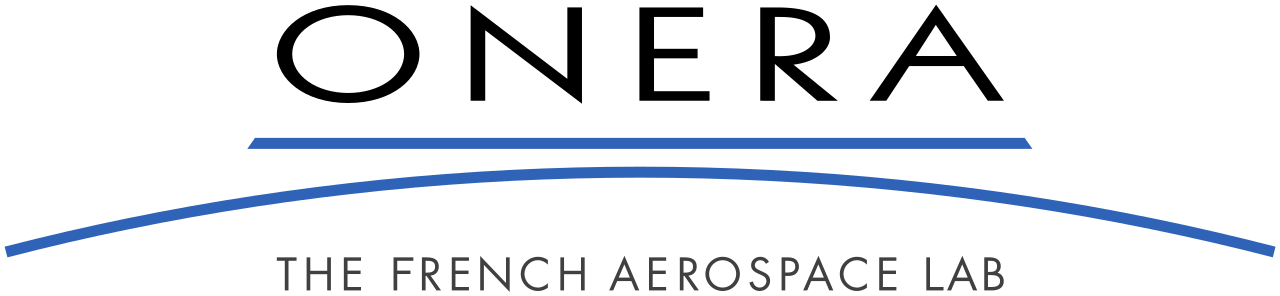
\includegraphics[height=1.5cm]{figures/01_intro/ONERA_logo.svg.png}\hfill
\includegraphics[height=1.5cm]{figures/01_intro/Logo-ISAE-SUPAERO.png}\par
	\vspace{4\baselineskip}
	{\Huge\scshape 
	\@title\par}
	\vspace{4\baselineskip}
	{\LARGE\@author\par}
	\vspace{4\baselineskip}
	{% author
	\fontsize{12}{14}\selectfont
	\bfseries\@titlepageauthor
	\par
 	}%
	\medskip
	{% address
		\fontsize{11}{12}\selectfont
		\def\and{\\\vspace{13pt}}
		\normalfont\@address
		\par
	}%
	\@date
	\vfill
	{\Large \@titlehead}\par
	\medskip
	\@publishers
\end{titlepage}

\newpage
\vspace*{\fill}
{\large \textbf{Colophon}} \\
This document was typeset with the help of \href{https://sourceforge.net/projects/koma-script/}{\KOMAScript} and \href{https://www.latex-project.org/}{\LaTeX} using the \href{https://github.com/fmarotta/kaobook/}{kaobook} class. \par
\medskip
\@publishers

\makeatother
%----------------------------------------------------------------------------------------
%	PREFACE
%----------------------------------------------------------------------------------------



%----------------------------------------------------------------------------------------
%	TABLE OF CONTENTS & LIST OF FIGURES/TABLES
%----------------------------------------------------------------------------------------

\begingroup % Local scope for the following commands

% Define the style for the TOC, LOF, and LOT
%\setstretch{1} % Uncomment to modify line spacing in the ToC
%\hypersetup{linkcolor=blue} % Uncomment to set the colour of links in the ToC
\setlength{\textheight}{230\vscale} % Manually adjust the height of the ToC pages

% Turn on compatibility mode for the etoc package
\etocstandarddisplaystyle % "toc display" as if etoc was not loaded
\etocstandardlines % "toc lines as if etoc was not loaded

\tableofcontents % Output the table of contents

\listoffigures % Output the list of figures

% Comment both of the following lines to have the LOF and the LOT on different pages
\let\cleardoublepage\bigskip
\let\clearpage\bigskip

\listoftables % Output the list of tables

% Comment both of the following lines to have the LOF and the LOT on different pages
\let\cleardoublepage\bigskip
\let\clearpage\bigskip

\printglossary[type=\acronymtype,title={List of Abbreviations}]
\endgroup

%----------------------------------------------------------------------------------------
%	MAIN BODY
%----------------------------------------------------------------------------------------

\mainmatter % Denotes the start of the main document content, resets page numbering and uses arabic numbers
\setchapterstyle{kao} % Choose the default chapter heading style

% \chapter*{Abstract}
\phantomsection
\addcontentsline{toc}{chapter}{Abstract}%
\markboth{Abstract}{Abstract}%
In the aerospace industry, an ongoing demand exists for lighter aerostructures, motivated by the imperative to enhance fuel efficiency and overall performance. For that reason, the aerospace sector is currently witnessing two innovative shifts: the transition to hydrogen-powered and electric planes, directing engineering efforts toward cleaner and more sustainable aviation technologies. These changes offer opportunities to deviate from the classic tube-and-wing configuration and explore inventive concepts like the flying wing or transonic truss-braced wings. One promising approach to meet these requirements is the utilization of lattice structures. These structures not only offer ultralight properties but also modularity. Modular designs bring numerous advantages, including the ability to assemble large structures from smaller and easier-to-manufacture repeating modules, on-field reparability, and rapid assembly for temporary structures.
The objective of this thesis is to develop a design and optimization algorithm for ultralight and modular aerostructures. In the initial phase, we reviewed existing literature to identify the most suitable algorithm basis for optimizing monolithic (non-modular) structures. After a thorough comparison, we selected the Truss Topology Optimization (TTO) approach, an optimization method based on the use of bars as the discretizing element of the structure. However, the classic TTO formulation has limitations, such as the inability to address buckling constraints, consider multiple load cases, and ensure mechanical compatibility. To overcome these challenges, we proposed an innovative two-step optimization algorithm. In this approach, a relaxed problem is utilized to generate an initial solution, serving as the starting point for the optimization using a complete formulation.
The second part of the thesis focuses on adapting the proposed monolithic formulation to incorporate modular constraints. Initially, the emphasis is on optimizing the topology of a fully modular structure, where a single module is repeated throughout the entire design. We evaluate how hyperparameters, such as the number of subdomains and module complexity, affect the mechanical performance of the structure. Subsequently, we delve into a more complex scenario, optimizing multiple module topologies and their layout within the structure. This is achieved through a Discrete Material Optimization (DMO) approach, employing a gradient-based optimizer.
By addressing the challenges of lightweight design and modularity in aerostructures, this research aims to contribute to the ongoing evolution of aerospace technologies and advance the efficiency and performance of future aircraft.


\newpage
\chapter*{Introduction}
\phantomsection
\addcontentsline{toc}{chapter}{Introduction}
\markboth{Introduction}{Introduction}%
\glsresetall % reset glossary



\textit{Scientists study the world as it is,}\\
\textit{Engineers create the world that never has been.} \vspace{5pt} \\
--- Theodore von K\'arm\'an \\

\section*{Towards lighter structures}

In the aerospace industry, an ongoing demand exists for lighter aerostructures, motivated by the need to enhance fuel efficiency and overall performance. This emphasis on lighter structures and materials not only reduces operational costs for airlines but also aligns with a broader commitment to sustainability, mitigating fuel consumption and carbon emissions. Furthermore, the aerospace sector is currently witnessing two innovative shifts: the transition to hydrogen-powered and electric planes, directing engineering efforts toward cleaner and more sustainable aviation technologies. These changes offer opportunities to deviate from the classic tube-and-wing configuration and explore inventive concepts like the flying wing \gls{bwb}, in which the fuselage and the wing blend to form an aircraft in which the fuselage, widened and integrated into the wing, also contributes significantly to the lift, or transonic truss-braced wings, with the goal of direct reduction in the aerodynamic drag by using a high-aspect ratio strut-braced wing configuration (see examples in \figref{fig:01_concepts}). Regardless of the specific configuration, a highly probable shared goal is the necessity to redesign lightweight dry--\ie with no fuel tanks inside--wings with high aspect ratios and thin profiles.

\begin{figure*}
    \hspace*{\fill}
    \subcaptionbox{}{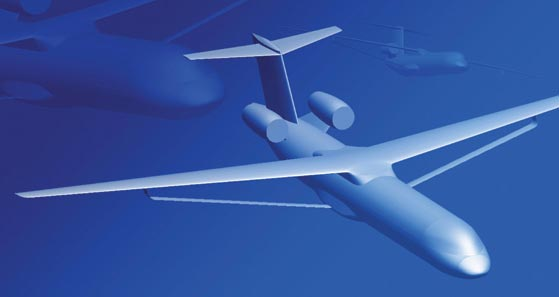
\includegraphics[height=4.3cm]{figures/01_intro/albatros-1.jpg}}
    \hfill
    \subcaptionbox{}{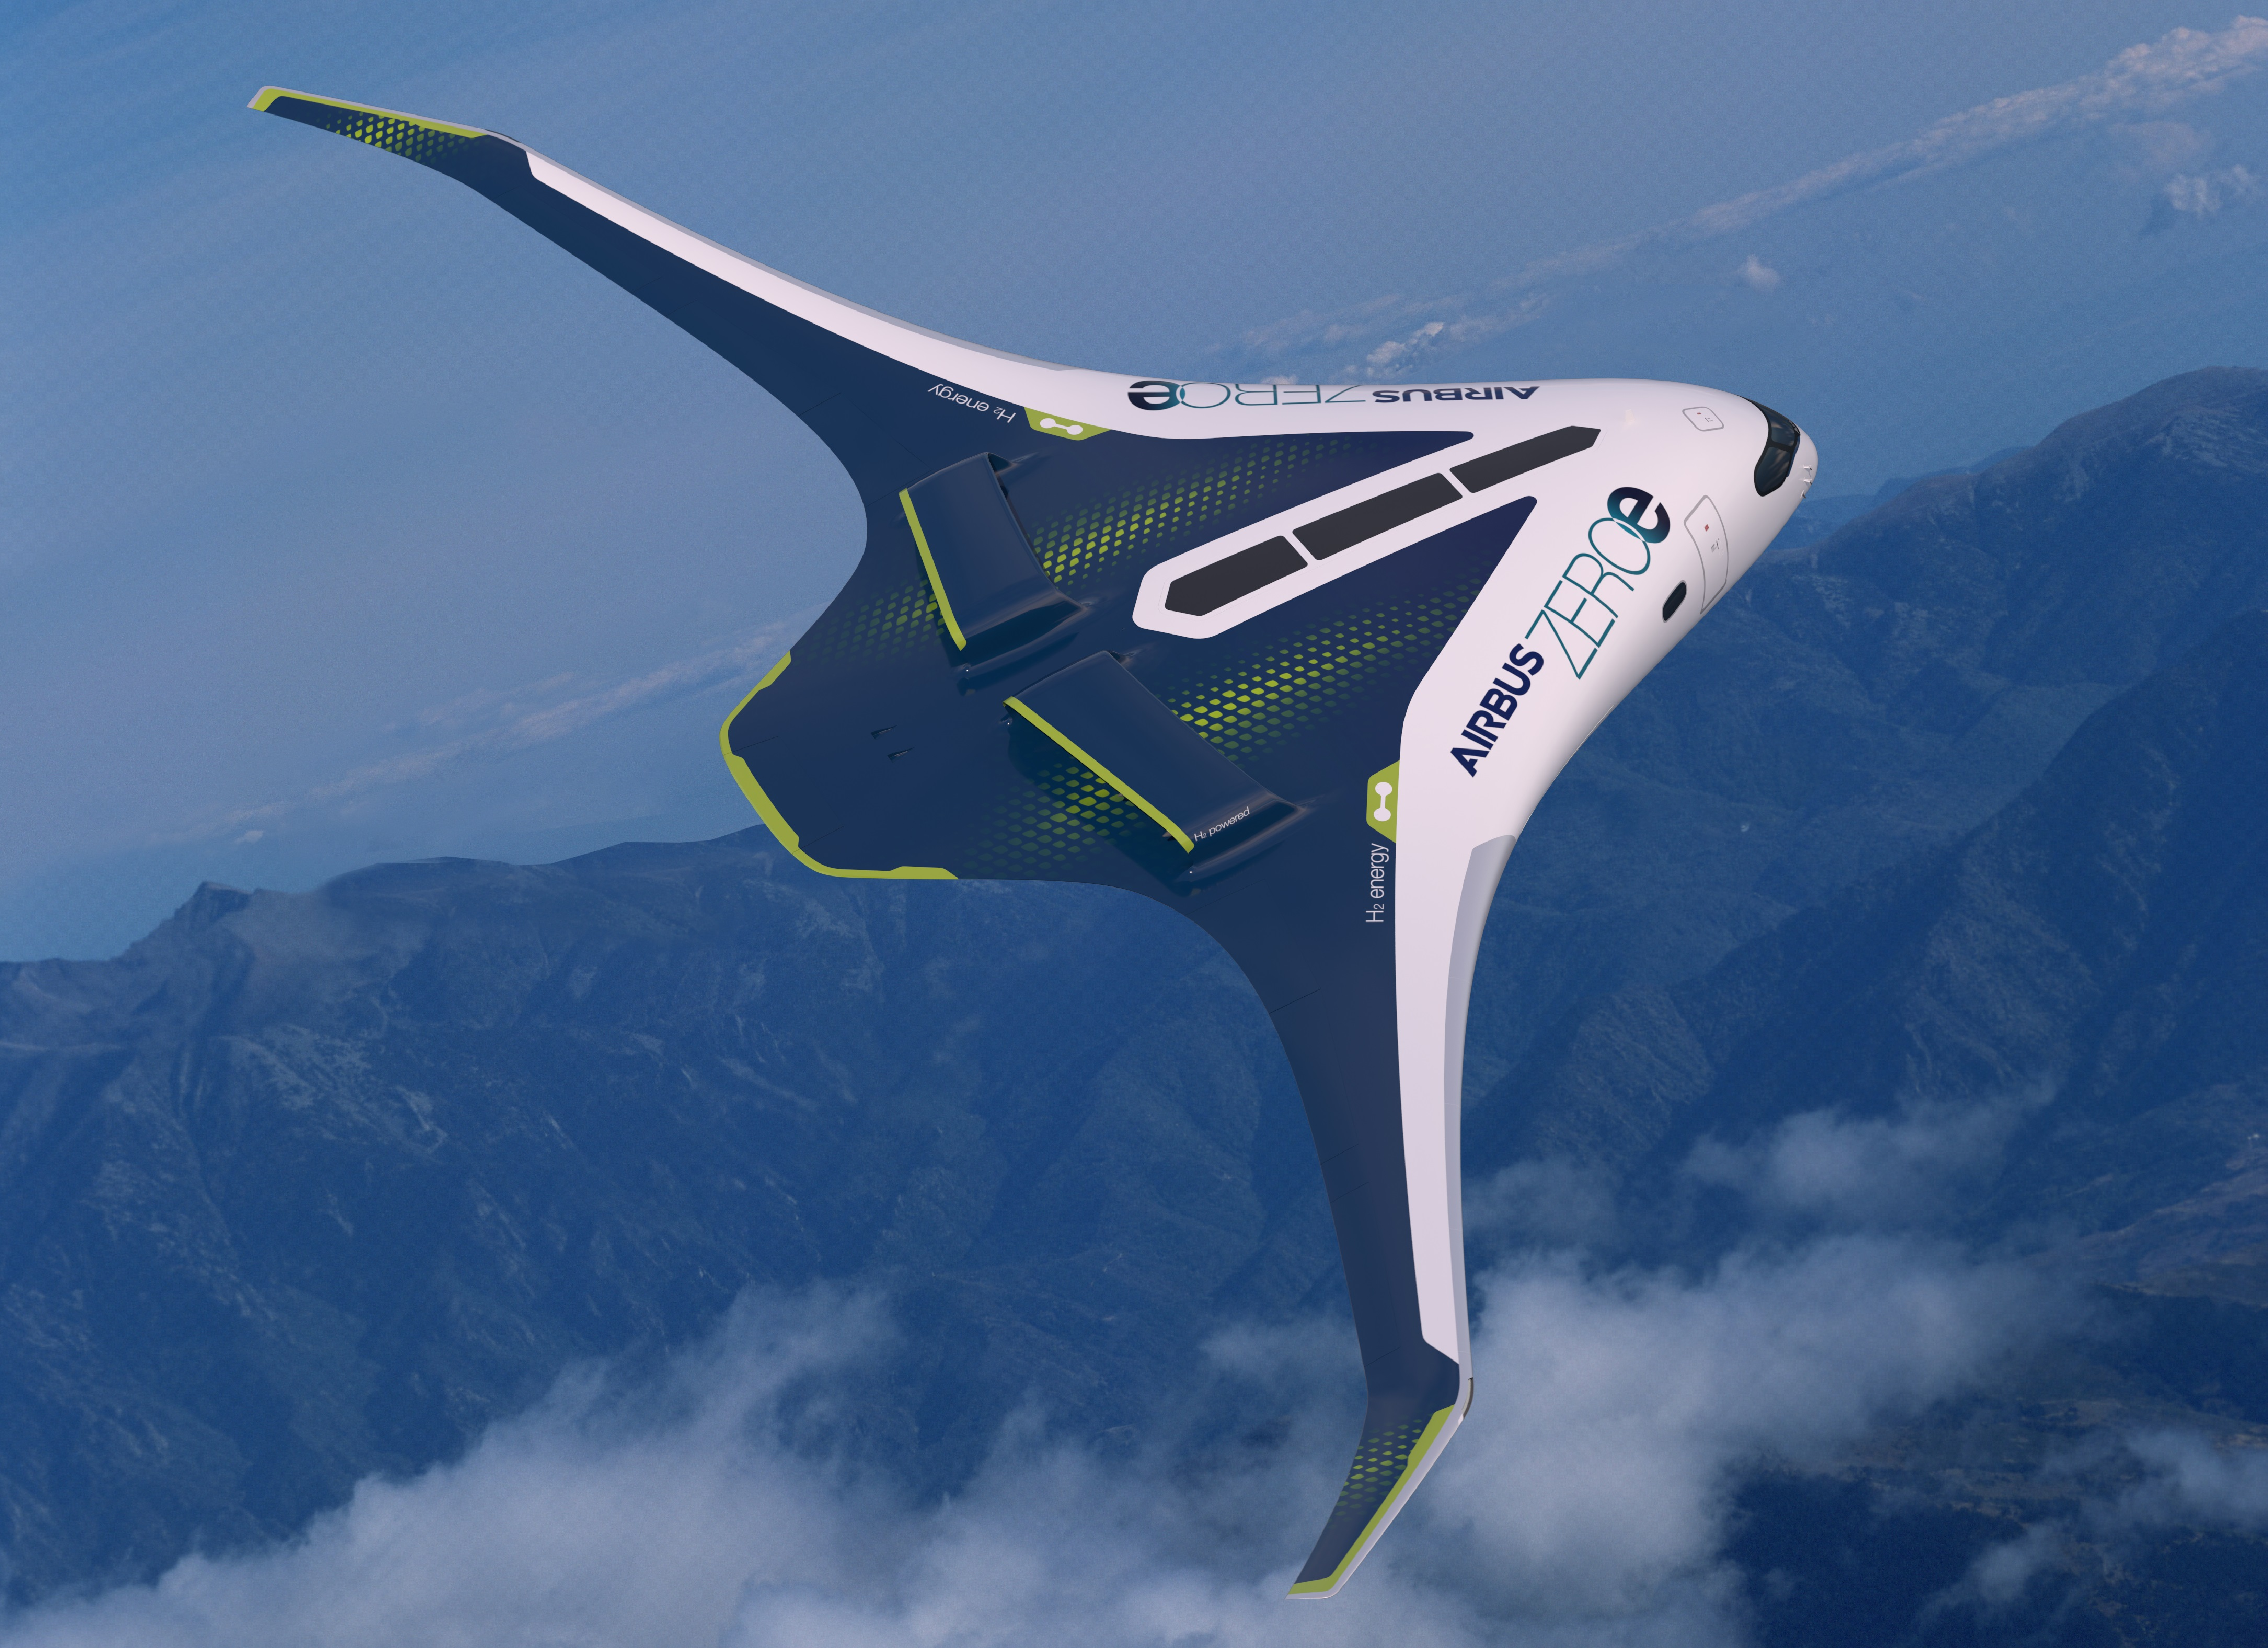
\includegraphics[height=4.3cm]{figures/01_intro/pm_38_529_529759-gml5anffhc.jpg}}
    \hspace*{\fill}
    \caption{(a) The transonic truss-braced wing called ALBATROS by ONERA \cite{carrier_investigation_2012,carrier_multidisciplinary_2021}; (b) the \acrfull{bwb} zero-e demonstrator by Airbus \cite{noauthor_airbus_2021}.}
    \label{fig:01_concepts}
\end{figure*}

To meet these criteria, a promising solution involves the application of lattice structures. Not only do these structures provide the necessary ultralight properties, but they also offer modularity. Modular designs come with several advantages, notably, the capability to construct large structures using smaller, more easily manufactured repeating modules. Other notable properties include on-field reparability, improved damage resistance, fast assembly for temporary structures, and stochastic error detection and repair compared to conventional monolithic material systems \sidecite{belvin_space_2016}. Additionally, recent research opens up the possibility of a fully robotic assembly phase, permitting faster and more reliable assembly (see \figref{fig:01_fab}).

\begin{figure}
    \hspace*{\fill}
    \subcaptionbox{}{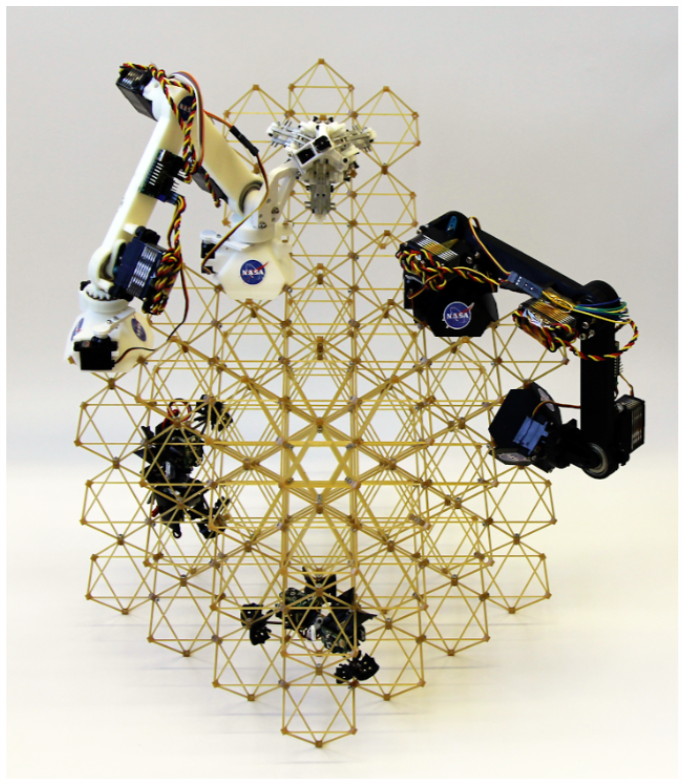
\includegraphics[height=3.5cm]{figures/01_intro/fab.png}}
    \hfill
    \subcaptionbox{}{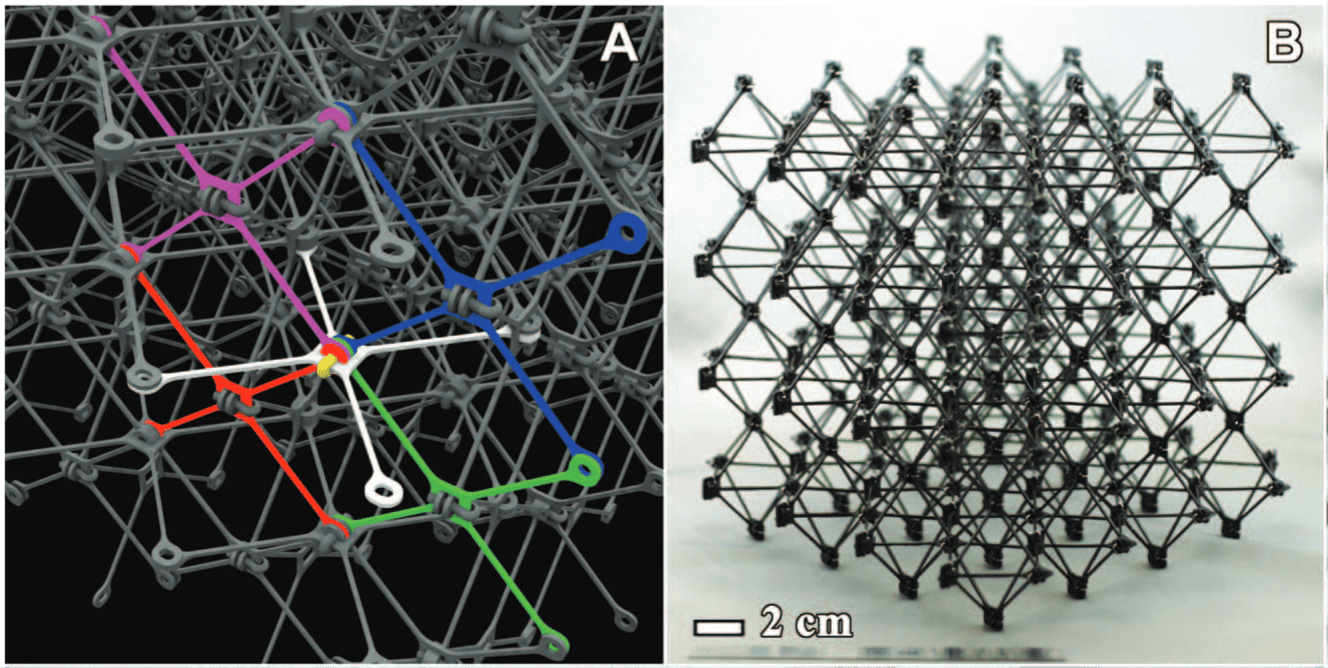
\includegraphics[height=3.5cm]{figures/01_intro/assembly.png}}
    \hspace*{\fill}
    \caption{\cite{cheung_reversibly_2013} \cite{costa_algorithmic_2020}.}
    \label{fig:01_fab}
\end{figure}

Optimizing lattice structures involves four main dimensions: material, module shape, layout, and topology. Material optimization focuses on improving mechanical properties by tailoring the distribution of lattice constituents, while shape optimization fine-tunes individual module external geometries. Layout optimization arranges modules in space, defining their presence or absence, and topology optimization refines the overall arrangement and connections within each module. Navigating these dimensions enables engineers to tailor lattice structures for a balance between weight, strength, and functionality. However, the abundance of design choices poses a significant challenge due to the lack of a standardized design method. Navigating this intricate landscape requires a systematic and efficient approach to ensure the resulting lattice structure meets specific engineering requirements. 

\section*{Objective}
This thesis aims to develop an optimization formulation and algorithm specifically designed for ultralight and modular aerostructures within the aerospace industry. In this field, reducing weight is crucial for improving overall performance. However, the introduction of modularity, while offering advantages such as manufacturing easing or improved damage resistance, may potentially lead to an increase in the overall weight of the structure when compared to classic monolithic structures. Consequently, the primary objective throughout this thesis is to develop an optimization method that not only harnesses the benefits of modularity but also ensures that the resultant structure remains as lightweight as possible. Striking a balance between the manufacturing advantages conferred by modularity and the critical need for weight reduction forms the central focus of this research.

\section*{Outline of the thesis}
The remainder of the thesis is structured as follows. \chpref{chap:02} provides a comprehensive review of structural optimization algorithms, especially focusing on ultralight weight and modular cases. The chapter introduces density-based topology optimization and the \gls{tto} formulations that will be utilized throughout the document. \chpref{chap:03} delves into a detailed comparison of the topology optimization methods, emphasizing results obtained when optimized structures exhibit a very low volume fraction, \ie less than \qty{5}{\percent}. A shared volume minimization with stress constraints formulation is presented, and a comparison is conducted by varying the material mechanical properties to achieve different volume fractions. After careful analysis, the \gls{tto} approach is selected due to its reduced computational time and suitability for modeling lightweight structures. \chpref{chap:04} addresses the limitations of the classic \gls{tto} formulation, such as the absence of local buckling constraints, minimum slenderness limits, consideration of multiple load cases, and ensuring mechanical compatibility for complex structures. To overcome these challenges, an innovative volume minimization formulation is proposed, incorporating the additional constraints needed to optimize real-world structures. Due to the inherent multimodality of the formulation, a two-step optimization algorithm is introduced, utilizing a relaxed problem to generate an initial approximate solution for subsequent optimization using a complete formulation. The Reinitialization heuristic is also proposed to reduce the influence of the starting point on optimization results. \chpref{chap:05} explores the incorporation of modular constraints in the proposed \gls{tto} formulation, employing the full-scale variable linking approach. This approach repeats a single module throughout the entire design to create optimized modular structures. The chapter evaluates the impact of hyperparameters, such as the number of subdomains and module complexity, on the mechanical performance of the structure. A \gls{doe} based on the chapter's results guides on choosing hyperparameters for optimization. In \chpref{chap:06}, the optimization scenario becomes more complex by introducing an additional optimization variable: the addition of multiple different topology modules. This optimization, inherently more complex, involves optimizing not only the modules' topology but also the layout of the modules within the structure. A modified \gls{dmo} approach is employed, utilizing a gradient-based optimizer, while the starting point is determined by employing k-means clustering on the stress distribution of the unoptimized initial structure. Up to this point, the focus has been on academic two or three-dimensional test cases. \chpref{chap:07} extends the application of the proposed optimization formulation and algorithms to the aerospace domain. Initially, the monolithic optimization algorithm is used to reduce the weight of the wingbox of the \gls{crm}, a standard benchmark for aeronautic research. The test case is subjected to multiple load cases (+2.5g, -1g, and cruise loads) associated with some correspective safety factors. The optimization is conducted using different materials and discretizations, resulting in lighter structures in less time compared to the literature. Later, the modular optimization formulation presented in \chpref{chap:06} is used on a drone-sized wing based on the 0012 NACA wing profile. Additionally, follow-up scientific perspectives are discussed.

% \setchapterpreamble[u]{\margintoc}
\glsresetall % reset glossary

\chapter{Literature review} \label{chap:02}
This thesis focuses on numerical optimization in the structural engineering domain. Consequently, it requires familiarity with existing optimization methods and contemporary engineering practices. The purpose of this chapter is to provide the reader with a non-exhaustive historical overview of structural optimization, particularly in the context of ultralight and modular structures. Additionally, we introduce crucial concepts and terminology that will be employed consistently throughout the document.

\section{An introduction to structural optimization}
Structural optimization is a multidisciplinary field within engineering that aims to systematically improve structural performance--considering factors like mass, stiffness, and dynamic response--by optimizing their shape, material distribution, and overall design. Historically, structural optimization algorithms are categorized into three families: sizing, shape, and topology optimization. Sizing optimization concentrates on determining the optimal distribution of variables, where both the design and state variable domains are known \textit{a priori} and remain constant during optimization. In contrast, shape optimization aims to discover the optimal shape of a predefined domain, treating the domain itself as a design variable allowing for flexibility in shaping the structure. Topology optimization goes further, involving the determination of features like the number, location, and shape of holes, as well as the connectivity of the structural domain. This approach offers a more comprehensive exploration of possibilities in structural design. A visual representation of the three families is provided in \figref{fig:02_opt_fam}.

\begin{figure}
    \centering
    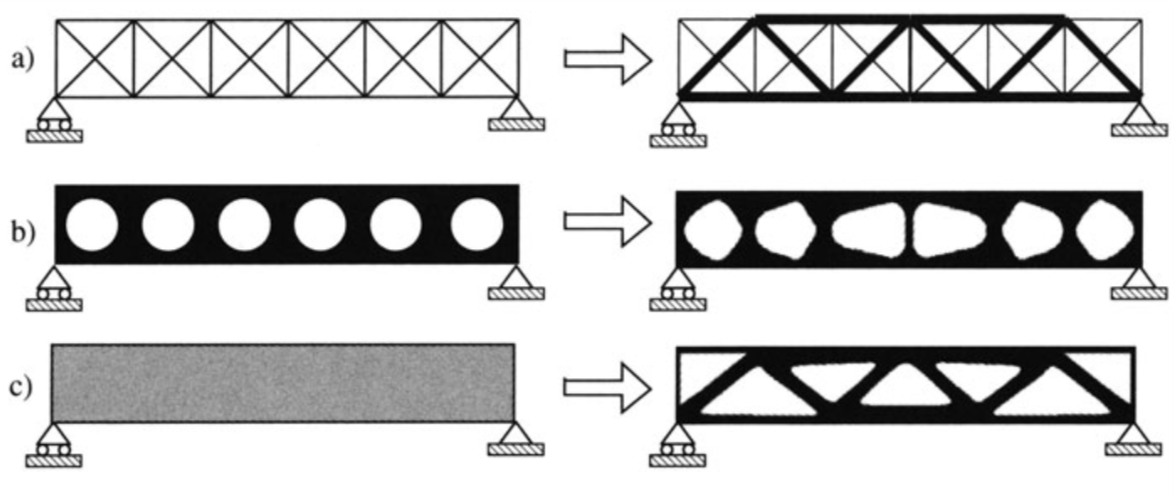
\includegraphics[width=\linewidth]{figures/02_literature/opt_family.png}
    \caption{Visual representation of (a) size, (b) shape, and (c) topology optimization \cite{bendsoe_topology_2004}.}
    \label{fig:02_opt_fam}
\end{figure}

Structural optimization involves using mathematical algorithms, computational models, and iterative analyses to explore and refine design solutions. For that reason, we introduce the basic concepts and terminology behind numerical optimization. In numerical optimization, algorithms are employed to minimize or maximize a specific function by adjusting various design variables. The problem may or may not be subject to constraints. Formulating an optimization problem is a crucial step to prevent common conceptual errors, such as confusing constraints with objective functions. An incorrect problem formulation can lead to a failed solution or yield a mathematical optimum that lacks feasibility from an engineering perspective.

The most general formulation of an optimization problem is written as:
\begin{equation}
    \begin{aligned}
    \min_{\vect{x}}         && & f(\vect{x})\\
    \textrm{by varying}   && \vect{x} &\in [l^-,l^+] \\
    \textrm{s.t.}   && \vect{g}_\text{e}(\vect{x}) &= 0 \\
    && \vect{g}_\text{i}(\vect{x}) &> 0, \\
    \end{aligned}
\end{equation}
where $ f(\vect{x}) $ is the objective function to minimize, $ \bm{x} $ is the vector of design variables bounded between $ l^- $ and $ l^+ $, and $\vect{g}_\text{e}$ and $\vect{g}_\text{i}$ represent the equality and inequality constraints, respectively.

\paragraph{Objective Function}
In numerical optimization, the objective function $f(\vect{x})$ represents the scalar that we aim to minimize. Should the goal be to maximize a function, one can achieve this by minimizing the opposite of that function, maintaining adherence to the convention. Common objective functions in structural design include the minimization of volume or structural compliance. The objective function can take the form of an explicit function or result from a highly complex computational procedure. The selection of the objective function is crucial to propose a design that is feasible from an engineering perspective, regardless of the precision of the optimization scheme employed.

Optimization problems are categorized in the literature based on how the objective function is with respect to design variables, whether linear, quadratic, or generally non-linear. It is possible to concurrently optimize multiple objective functions, but this usually results in a family of optimum designs with differing emphases on the various objectives called the Pareto front. When possible, it is more straightforward to convert these diverse objectives into constraints~\sidecite{martins_engineering_2021}.

\paragraph{Design Variables}
The design variables $\vect{x}$ are the parameters that the optimizer algorithm changes to minimize the objective function. Design variables could be continuous or discrete if only some distinct values are allowed (for example, only a certain size for a hole in a structural analysis). The optimization problem formulation allows for the lower and upper boundary for each design variable known in the literature as variable bounds.

\paragraph{Constraints}
The constraints are functions used to restrict the design variables in some way. They serve the purpose of preventing the algorithm from converging to a numerical minimum that is not feasible due to physical and engineering constraints. Similar to the objective function, constraint functions can take on linear, quadratic, or generally non-linear forms, and different algorithms must be applied accordingly.

Constraint functions can be further classified into two types: equality constraints ($\vect{g}\text{e}$), which arise when the design variables are restricted to be equal to a fixed quantity, and inequality constraints ($\vect{g}\text{i}$), which come into play when the design variables are required to be greater than or equal to a certain quantity.

\subsection{Optimizers}
The field of numerical optimizers is extensive. For that reason, our focus here will be specifically on algorithms employed in structural optimization. Various algorithm types have been applied to address structural optimization problems, predominantly categorized into three main families: optimality criteria, metaheuristic algorithms, and gradient-based strategies.

\gls{oc} refer to mathematical conditions or rules used to assess and guide the modification of a design or structure to achieve the desired performance~\sidecite{prager_problems_1968,prager_optimality_1968}. In the context of topology optimization, \gls{oc} are primarily applied in compliance minimization problems, as each element contributes independently to the overall compliance. Bendsøe used \gls{oc} to seek the stiffest plate \ie compliance minimization--that can be made of a given amount of material and, together with Kikuchi~\sidecite{bendsoe_generating_1988}, they used \gls{oc} to obtain optimal shape design of structural elements based on boundary variations without the use of remeshing. Later, Bendsøe and Sigmund~\sidecite{bendsoe_optimization_1995,sigmund_99_2001} introduced a heuristic update scheme for isotropic materials, while Allaire \etal~\sidecite{allaire_homogenization_1996} demonstrated the convergence proof for both isotropic and anisotropic materials using the \gls{ad} approach. In both methods mechanical analysis provides essential information for solving closed-form conditions, allowing iterative updates of variables until convergence is achieved. Recently, \gls{oc} methods gained interest again thanks to the reduced calculation time~\sidecite{li_accelerated_2020, ferrari_new_2020} obtained using a modified Anderson acceleration strategy~\sidecite{anderson_iterative_1965}.

Metaheuristic (or gradient-free) algorithms offer a broader range of options compared to their gradient-based counterparts. While gradient-based algorithms typically conduct local searches, possess mathematical justification, and operate deterministically, metaheuristic algorithms are simpler and usually take much less developer time to use, and are perfect candidates for smaller problems. They find very diverse application cases and are useful when the design space is discrete, with multiple objective functions, or highly non-linear with many local minima (multimodal). The works authored by Conn \etal~\sidecite{conn_introduction_2009} and Audet and Hare~\sidecite{audet_derivative-free_2017} offer a comprehensive exploration of gradient-free optimization algorithms. Evolutionary algorithms, a prominent category, simulate natural selection by retaining the fittest solutions in each generation while introducing mutations or cross-overs for improvement. A review of these optimization methods is given in the following reference~\sidecite{simon_evolutionary_2013}. These algorithms, also called \gls{ga}, are employed for example by Balamurugan \etal~\sidecite{balamurugan_two_2011} for compliance minimization, showcase versatility but face challenges with combinatorial considerations as the number of design variables increases~\sidecite{sigmund_usefulness_2011}. Particle swarm and ant colony algorithms, inspired by nature, provide alternative strategies with randomness and new search directions. However, these non-gradient methods require regularization schemes for topology optimization, as outlined by Luh, Lin, and others~\sidecite{luh_structural_2009, luh_binary_2011}.
Targeting the resolution of \gls{mip} problems, branch-and-bound algorithms divide the feasible set of the original problem into subsets through a process known as branching. These subsets are then further segmented to refine the partition of the feasible set. For each subset, lower bounds and optionally upper bounds on the objective function value are determined, a process referred to as bounding. Typically, the lower bounding problems are convex problems that can be efficiently solved to global optimality. Stolpe~\sidecite{stolpe_global_2004} addresses a volume minimization problem on a truss using a continuous branch-and-bound method, ensuring convergence to a globally optimal solution. The \gls{eso} framework, initially a metaheuristic, removes less solicited elements iteratively~\sidecite{mattheck_new_1990, xie_simple_1993}. These methods offer freedom in optimization and improved convergence to local minima, especially in handling various optimization problems like buckling~\sidecite{manickarajah_evolutionary_1998}. The \gls{eso} algorithm has been enhanced by the \gls{beso} framework~\sidecite{young_3d_1999}, which allows both removal and addition of elements. 

Gradient-based algorithms in optimization leverage local information at a trial point to comprehend the shape of the local objective function in the neighborhood. This insight is crucial for determining the optimal direction to minimize the objective function. Typically, only the Jacobian (first derivative) is utilized, though more advanced algorithms incorporate the Hessian (second derivative). The computational demand for gradient calculation often constitutes the most resource-intensive aspect of the optimization loop. When constraints are present, solving the problem directly on the analytic response surface of the objective function becomes impractical. Consequently, the approach involves creating local approximations of the problem at the current design point using gradient information. These approximations are designed so that specialized algorithms can efficiently solve them. The categorization of gradient-based algorithms is often based on how this local approximation is constructed.

The most used approximations in structural optimization includes among others \gls{slp}, \gls{sqp} and \gls{slsqp}~\sidecite{kraft_software_1988}, \gls{mma}~\sidecite{svanberg_method_1987} and its amelioration \gls{gcmma}~\sidecite{svanberg_class_2002} and \gls{gbmma}~\sidecite{bruyneel_family_2002}, and \gls{conlin}~\sidecite{fleury_structural_1986}. Specialized algorithms for solving the approximated problems are, among others, the primal-dual method and interior-point method.

An interior-point method is a numerical optimization algorithm used to solve constrained optimization problems. The key idea behind interior-point methods is to transform the constrained optimization problem into a sequence of unconstrained problems, allowing for efficient iterative solutions. The method introduces a barrier function that penalizes points outside the feasible region, effectively creating a "barrier" against leaving that region. This barrier function is incorporated into the objective function, and as the optimization progresses, it guides the search towards the interior of the feasible region. The term "interior point" originated from early methods that relied on interior penalty techniques, assuming the initial point was feasible. Nevertheless, contemporary interior-point methods such as the open source IPOPT~\sidecite{wachter_implementation_2006} are more versatile and can start from infeasible points. Rojas Labanda and Stolpe conducted a benchmark of various optimization algorithms and structural optimization formulations using a compliance minimization problem. Their findings highlight the efficacy of employing interior-point algorithms such as IPOPT in topology optimization problems~\sidecite{rojas_labanda_benchmarking_2015}.

\section{Ultra-lightweight structures optimization approaches}
Two of the most frequently employed formulations for structural optimization are the minimization of volume while adhering to stress constraints and the minimization of compliance under volume constraints. Historically, the volume minimization formulation has been used in the first works of structural optimization of truss structures~\sidecite{dorn_automatic_1964,chan_optimum_1964,hemp_optimum_1973}. The problem was initially formulated in terms of member forces, ignoring the kinematic compatibility to obtain a \gls{lp} problem. The formulation was modeled using the \gls{sand} approach, in which the equations of nodal equilibrium are treated as equality constraints, and where both nodal displacements and the cross-sectional areas of truss members serve as design variables~\sidecite{sankaranarayanan_truss_1994}. These methods are known in the literature as layout optimization or \gls{tto}. 

However, to attain greater design freedom, the structure optimization field later transitioned from truss structures to continuous discretization (also called density methods). While truss structures offered simplicity and ease of analysis, they imposed limitations on the design due to their discrete member configurations and their inability to transmit moments, handle torsional effects, and represent complex structural elements such as plates or volumes. The continuous mesh offered instead more versatility~\sidecite{bendsoe_generating_1988,bendsoe_optimal_1989}, and has since been used for multiple different applications, \eg the design of optimized repetitive metamaterials~\sidecite{sigmund_materials_1994, zhang_scale-related_2006,collet_topology_2018}, fluids optimization~\sidecite{borrvall_topology_2003}, modelization of self-weight of the structure~\sidecite{bruyneel_note_2005}, the simulation of advanced manufacturing constaints~\sidecite{sigmund_manufacturing_2009,brackett_topology_2011}, the design of compliant mechanism~\sidecite{sigmund_design_1997, bruns_topology_2001}, or the optimization for additive manufacturing~\sidecite{wang_space-time_2020}. Other than the density methods, other ways to deal with topology optimization exist, like level-set methods \sidecite{allaire_level-set_2002,wang_level_2003,allaire_structural_2004}. The \gls{sand} approach is, however, incompatible with density methods due to its excessive number of variables\sidenote{This proposition holds when referring to the end of the 1980s when computational power was scarce compared to what we have today.}. Given this limitation, a new approach was required to better handle the complexity of continuous meshes.

In the density-based \acrfull{nand} approach, the nodal displacement (state) variables are eliminated from the optimization problem through a process where the structural equilibrium equation is solved every iteration of the optimization loop instead of being used as a constraint of the optimization. This results in an independent nested phase where the state equation of structural equilibrium is solved separately from the optimization algorithm. This creates a dense coupling between displacement and material density variables, necessitating a computationally expensive sensitivity analysis within the nested algorithm, typically employing the adjoint method (more information about the adjoint method on the following resurces~\sidecite{tortorelli_design_1994,martins_engineering_2021}). Nevertheless, if the problem is reformulated as a compliance minimization with volume constraints, the problem is self-adjoint and the adjoint algorithm is no longer necessary to evaluate the gradient sensitivities~\sidecite{bendsoe_topology_2004}, and this reduces considerably the computational times.

Both the \gls{tto} methods based on the ground structure and the density-based topology optimization approaches are good candidates for the optimization of ultra-light structures. We review here their main characteristics and numerical properties, starting from density-based approaches.

% The introduction of new propulsion technologies (electric, LH2) aimed at reducing greenhouse gas emissions in the aeronautical sector provides an opportunity to rethink the structure design from the initial phases. The subsequent reevaluation of associated design methods has led to the exploration of structural optimization techniques. Topology optimization, in particular, offers a valuable approach to identifying optimal shapes and material distributions and allows achieving any shape within the design space instead of dealing with predefined configurations. Classical topology optimization considers the design domain as a continuum, in which each location may or may not have a material assigned to it~\cite{bendsoe_optimal_1989}. While topology optimization offers tremendous benefits in terms of weight reduction and structural efficiency, it is important to acknowledge the challenges associated with manufacturing such designs. The intricate and complex geometries generated through the optimization can pose difficulties in the fabrication process, often requiring advanced manufacturing techniques, specialized equipment, and specific constraints in the optimization \cite{zhou_progress_2002,brackett_topology_2011,liu_current_2018}. Additionally, the computational time required for generating such optimized designs, particularly for low-volume fractions typical of the aerospace domain, can be significant \cite{aage_giga-voxel_2017}, impacting the overall efficiency of the design process. This remains true even with the use of adaptive meshes~\cite{salazar_de_troya_adaptive_2018, zhang_adaptive_2020}.

\subsection{Density-based topology optimization}

\begin{marginfigure}
    \centering
    \includegraphics{figures/02_literature/01_contin_mesh/c_mesh.pdf}
    \caption{The domain $\Omega$ is discretized using $N_\text{e}=N_\text{x} N_\text{y}$ continuous 4-nodes elements.}
    \label{fig:02_mesh_c}
\end{marginfigure}
Let $\Omega \in \mathbb{R}^2$ be a rectangular domain of dimensions $X$ and $Y$, containing respectively $N_\text{x}$ and $N_\text{y}$ linear 4-nodes elements, for a total of $N_\text{e}=N_\text{x} N_\text{y}$ elements and $M$ nodes (see \figref{fig:02_mesh_c}). The objective of the optimization is the minimization of the compliance $C$ of the structure, equivalent to finding the structure with the least possible nodal displacement with respect to a defined set of boundary conditions. 

\paragraph{Compliance minimization formulation} The Problem $\mathbb{T}_0$ is stated in terms of the density design variables $\vect{\rho}$ for a single load case as follows:
\begin{equation}
    \begin{aligned}
    \min_{\vect{\rho}}         && C &= \sum_{i} \vect{u}_{e,i}^T \matr{K}_{e,i} \vect{u}_{e,i}=\vect{f}^T\vect{u}&& \forall i \in [0,\dots,N_\text{e}]                         \\
    \textrm{s.t.}   && & \frac{1}{V_\text{p}}\frac{\sum_{i} \left(\rhophys_i v_i \right)}{V_0} - 1 \leq 0 && \forall i \in [0,\dots,N_\text{e}] \\
    && \matr{K}\vect{u} &= \vect{f} &&\\
    && 0 &\leq \rho_i \leq 1. && \forall i \in [0,\dots,N_\text{e}] \\
    \end{aligned}
    \tag{$\mathbb{T}_0$}
    \label{eq:02_prob-comp}
\end{equation}
The design variables $\vect{\rho}$ are defined for every element of the structure as $\vect{\rho} = [\rho_1, \rho_2, \ldots,\rho_{Ne}]^T$, with $\rho_i \in [0,1], \; \forall i \in [0,\dots,N_\text{e}]$. The physical densities $\vect{\rhophys}$ are related to the design variable $\vect{\rho}$ through density filtering and threshold projection~\sidecite{wang_projection_2011}, as explained later in the document. $V_\text{p}\in [0,1]$ is the prescribed volume fraction that acts as the constraint of the minimization problem, while $v_i$ represents the area of the $i$-th element and $V_0$ is the total area of the domain $\Omega$. $\matr{K}\vect{u} = \vect{f}$ is the state equation of the problem and defines the elastic response of the structure to an external nodal load $\vect{f}=[f_1, f_2, \ldots,f_{2M}]^T$. The global stiffness matrix $\matr{K}$ is assembled from the element stiffness matrix $\matr{K}_{e,i}$ and $\matr{K}_{e,i} = E_i \matr{K}_{e,0}$ where $\matr{K}_{e,0}$ represents the element stiffness matrix relative to the chosen type of element (linear or quadratic) and $E_i(\rhophys_i)$ the Young's modulus of the $i$-th element. 

The material scheme used to interpolate between void and full material is the well-known \gls{simp}~\sideciteonce{bendsoe_optimal_1989,bendsoe_material_1999} approach. It is governed by the equation:
\begin{equation}
    E_i(\rhophys_i) = E_{\textrm{min}} + \rhophys_i^p(E_0-E_{\textrm{min}}),
    \label{eq:02_simp}
\end{equation}
where the parameter $p$ penalizes the intermediate densities and pushes the result to a black-and-white result. $E_0$ is the Young's modulus of the dense material and $E_{\textrm{min}}$ is a small value used to avoid the global stiffness matrix $\matr{K}$ from being singular when $\rhophys_i=0$. 

The \gls{simp} exponent $p$ is constrained to be greater than or equal to 1. From a physical perspective, the extreme case of $p = 1$ makes sense only in a two-dimensional optimization context, where it becomes equivalent to optimizing membrane thickness. When $p > 1$, the interpolation results in an equivalent homogenized stiffness tensor for intermediate densities, determined by the material-to-void ratio $\rho$. This mirrors microstructures conforming to the \gls{hs} conditions, which estimate the theoretical lower and upper bounds for the elastic modulus of a homogeneous, isotropic mixture of different materials based on their elastic modulus and volume fractions \sidecite{hashin_variational_1963}. If the exponent $p$ exceeds 3, Bendsøe \sidecite{bendsoe_material_1999} mathematically proves that the equivalent homogenized stiffness tensor adheres to the upper bound of the \gls{hs} conditions (refer to \figref{eq:02_simp}). It is important to note that in the mono-scale topology optimization context, deviating from the \gls{hs} bounds for intermediate densities is allowed. The objective is to drive the density distribution towards a black-and-white result with minimal intermediate densities, without concerning whether the equivalent homogenized stiffness tensor can be replicated by a real microstructure.

\begin{figure}
    \centering
    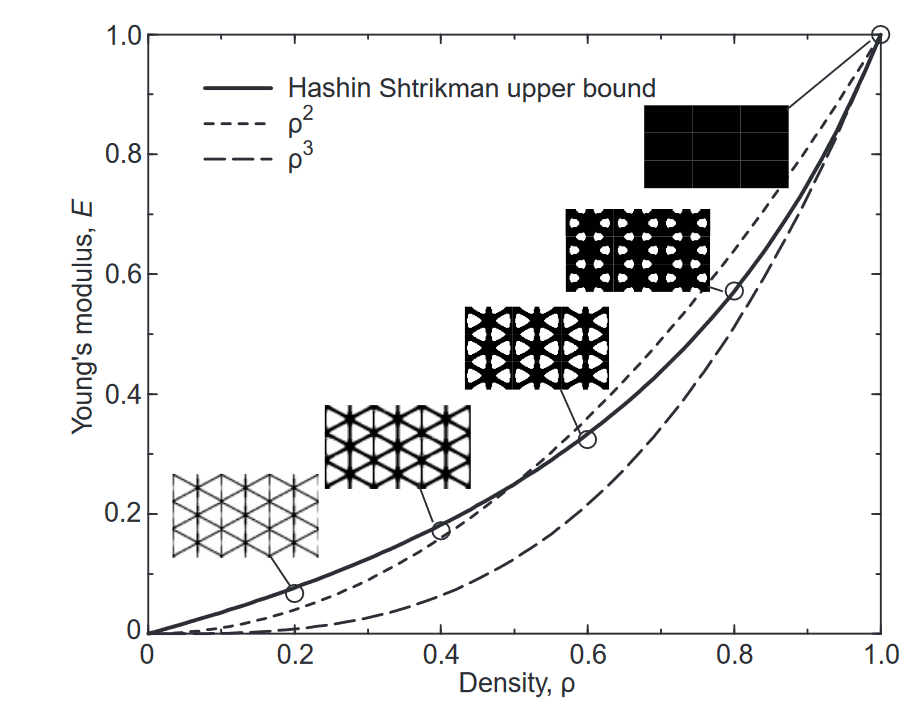
\includegraphics[width=0.75\linewidth]{figures/02_literature/simp.png}
    \caption{Comparison between SIMP model with the Hashin-Strikman upper bound, considering an isotropic material with a Poisson ratio of $1/3$ mixed with void. The Hashin-Strikman upper bound is illustrated with microstructures approaching the specified bounds. \cite{bendsoe_material_1999}.}
    \label{fig:02_simp}
\end{figure}

\paragraph{Spatial filtering and projection} 
Multiple approaches have been developed to solve the problems linked to mesh discretization, such as mesh dependency or the checkerboard problem~\sidecite{diaz_checkerboard_1995}. Filtering the sensitivity information of the optimization problem proved to be an effective approach to guarantee independence from mesh resolution~\sidecite{sigmund_design_1994,
sigmund_design_1997}. Another possibility is instead to directly filter the density field $\vect{\rho}$ using the 2D convolution operator~\sidecite{sigmund_morphology-based_2007}. The weight function $w$ (or kernel) of the convolution is defined as:
\begin{equation}
    w(d_j) = R - d_j, \quad j \in \mathbb{N}_{i,R}
\end{equation} 
where $\mathbb{N}_{i,R}$ represent the set of elements lying within a circle of radius $R$ centered on the $i$-th element and $d_j$ is the distance of the $j$-th element to the center of the filter (see \figref{fig:02_ker}).
\begin{marginfigure}
    \centering
    \includegraphics{figures/02_literature/02_circ_filter/filt_cir.pdf}
    \caption{Kernel of the 2D convolution operator.}
    \label{fig:02_ker}
\end{marginfigure} 
The filtered values $\vect{\rhofil}$ of the design variable $\vect{\rho}$  are calculated as:
\begin{equation}
    \rhofil_i = \frac{\sum_{j \in \mathbb{N}_{i,R}} w(d_j)v_j\rho_j}{\sum_{j \in \mathbb{N}_{i,R}} w(d_j)v_j}.
    \label{eq:02_rhofil}
\end{equation}
As the filtering phase produces a large number of gray elements, a projection technique based on the \textit{tanh} function is implemented~\sidecite{wang_projection_2011} to evaluate the value of the physical density $\vect{\rhophys}$  of the structure:
\begin{equation}
    \rhophys_j = \frac{\tanh(\beta\eta)+\tanh(\beta(\rhofil_j - \eta))}{\tanh(\beta\eta)+\tanh(\beta(1 - \eta))},
    \label{eq:02_proj}
\end{equation}
where $\beta$ is a parameter that defines the slope of this approximation function: the larger the value of $\beta$, the fewer elements with intermediate density are present in the structure topology. $\eta$ is the threshold value of the projection. The key characteristic of \eqref{eq:02_proj} is its smoothness over the defined interval, permitting easy differentiation and rendering it ideally suited for gradient descent optimization algorithms.

In the domain of structural topology optimization, it is a widely adopted strategy to employ continuation methods. Introduced in the 90s \sidecite{allaire_numerical_1993, allaire_topology_1993}, they are used to converge towards more optimized structures. These methods solve a sequence of problems with increasing values of the \gls{simp} material penalization parameter $p$. Many researchers such as Bendsøe and Sigmund \sidecite{bendsoe_topology_2004} and Rozvany \sidecite{rozvany_critical_2009} consider, among others, continuation methods as a standard procedure in topology optimization. However, this approach comes at the expense of an increased number of iterations and, consequently, augmented computational time \sidecite{petersson_slope_1998}. In an effort to mitigate this drawback, Rojas Labanda and Stolpe \sidecite{rojas-labanda_automatic_2015} have derived an automatic penalization scheme. This innovative scheme aims to reduce both the objective function value and the number of iterations, providing an improvement over the classical formulation with a fixed penalty parameter. While the literature is predominantly focused on the continuation scheme on the \gls{simp} material penalization parameter $p$, it is worth noting that similar techniques could be employed for other optimization parameters \eg the filter radius $R$ or the projection parameter $\beta$.

While density-based topology optimization offers tremendous benefits in terms of weight reduction and structural efficiency, it is important to acknowledge the challenges associated with manufacturing such designs. The intricate and complex geometries generated through the optimization can pose difficulties in the fabrication process, often requiring advanced manufacturing techniques, specialized equipment, and specific constraints in the optimization~\sidecite{zhou_progress_2002,brackett_topology_2011,liu_current_2018}. Additionally, the computational time required for generating such optimized designs, particularly for low-volume fractions typical of the aerospace domain, can be significant~\sidecite{aage_giga-voxel_2017}, impacting the overall efficiency of the design process. This remains true even with the use of adaptive meshes~\sidecite{salazar_de_troya_adaptive_2018, zhang_adaptive_2020}. Even if the freedom of the design space offered by continuous meshes is high, it is known that at very low volume fractions (\eg ultralight structures), and, especially if buckling constraints and manufacturing considerations (\eg minimum length scale), are taken into account, the optimal topology resembles a truss-like structure~\sidecite{sigmund_non-optimality_2016}. As a result, a distinct branch of continuous topology optimization has emerged specifically tailored for optimizing truss-like structures, known as feature-mapping topology optimization (also called topology optimization with explicitly defined components).

\subsection{Feature-Mapping topology optimization}
Topology optimization methods using explicitly defined components have been developed to permit an easier interpretation of the solution, finding the optimal shape, size, and connectivity of components projected over a finite element continuous mesh (see \figref{fig:03_to_component}). Two main feature-mapping methods applied to topology optimization have been developed~\sidecite{wein_review_2020}, the \gls{mmc} approach~\sidecite{guo_doing_2014,zhang_new_2017}
and the \gls{gp} approach~\sidecite{norato_geometry_2015, zhang_geometry_2016}, later combined in a unique methodology called \gls{ggp}~\sidecite{coniglio_generalized_2020}. Recently, the \gls{gp} approach has been used to optimize light lattice structures, proving the effectiveness of the method to provide easy-to-interpret solutions~\sidecite{kazemi_multi-material_2020}. Nevertheless, the optimization is still based on a density field projected on a continuous mesh, that needs to be refined to correctly discretize low-volume fraction structures. Additionally, truss structure design naturally depends on constraints on maximum allowable stress and buckling which are all known for being difficult to implement on topology optimization using the \gls{nand} formulation. This is principally due to the singular optima (or topologies) phenomenon~\sidecite{cheng_relaxed_1997,rozvany_design-dependent_2001} and the pseudo-modes of buckling of low-density elements~\sidecite{gao_topology_2015}. \begin{figure}
    \hspace*{\fill}
    \subcaptionbox{}{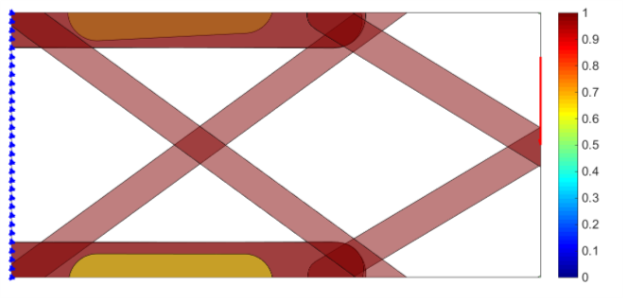
\includegraphics[width=0.45\linewidth]{figures/02_literature/coniglio1.png}}
    \hfill
    \subcaptionbox{}{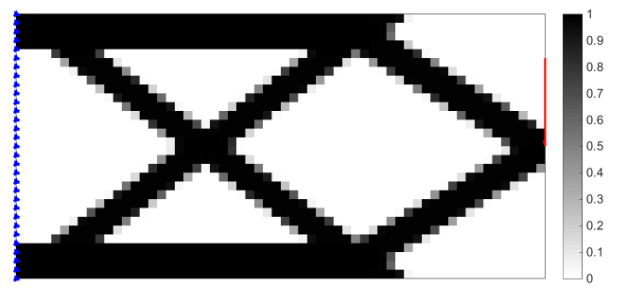
\includegraphics[width=0.45\linewidth]{figures/02_literature/coniglio2.png}}
    \hspace*{\fill}
    \caption{Component (a) and density (b) plot of a short cantilever beam optimized using the component-based topology optimization method \gls{ggp}~\cite{coniglio_generalized_2020}.}
    \label{fig:03_to_component}
\end{figure}

\subsection{Truss topology optimization (TTO)} \label{sec:02_tto}
\acrfull{tto} focuses on optimizing the topology of the truss structure itself, instead of operating on a continuous mesh. It involves selecting the cross-sectional areas and the connectivity of a discrete and dense mesh called ground structure, aiming to minimize weight while satisfying structural constraints. The process is graphically presented in \figref{fig:02_tto_ex}.

\begin{figure}
    \centering
    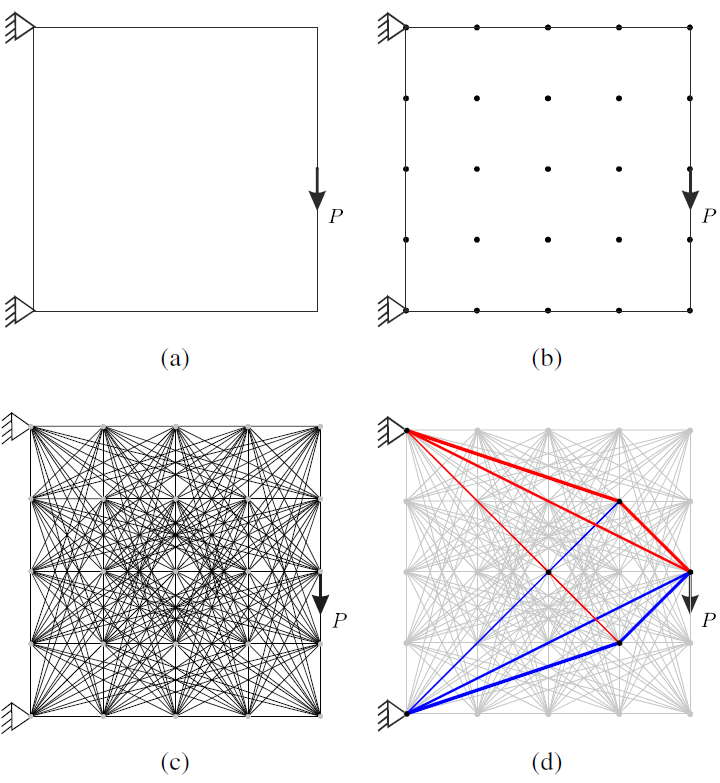
\includegraphics[width=0.7\linewidth]{figures/02_literature/layopt.png}
    \caption{The TTO algorithm is divided into four principal steps: (a)
    specification of the design space, loads, and boundary conditions; (b) discretization
    of the design space; (c) the ground structure is generated depending on the
    desired connectivity level; (d) resolution of the optimization problem and plot of
    the solution \cite{he_python_2019}.}
    \label{fig:02_tto_ex}
\end{figure}

In the early works, the \gls{tto} problem was formulated in terms of member forces~\sidecite{dorn_automatic_1964, hemp_optimum_1973} with plastic material modelization, ignoring the kinematic compatibility to obtain a \gls{lp} problem. Formulated using the \gls{sand} approach, the equations of structural mechanics of the problem are imposed as constraints of the optimization and, contrary to \gls{nand} approaches, are not explicitly solved. Formulated that way, it is trivial to add maximum stress constraints compared to an equivalent \gls{nand} formulation. However, the \gls{sand} formulation with plastic material modelization only correctly predicts the mechanical behavior of statically determinate structures or mechanisms~\sidecite{kirsch_optimal_1989, rozvany_layout_1995}. Moreover, adding local buckling constraints to the optimization formulation is fundamental, as ultralight truss structures are often dominated by this mode of failure~\sidecite{sigmund_non-optimality_2016}. Multiple works in the field of truss structure optimization have focused on addressing these two crucial challenges~\sidecite{kirsch_optimal_1980,cheng_aspects_1995,achtziger_local_1999}.

\paragraph{Classical Michell structures} \label{sec:02_michell}
The characteristics of this class of truss structures are described by some simple criteria that date to the end of the 19th and the beginning of the 20th century. When a structure is statically determinate — \ie the structure is not a mechanism, and it is not over-constrained by the supports — the Maxwell theorem~\sidecite{maxwell_ireciprocal_1870} states that:
\begin{equation} \label{eq:02_maxwell-th}
    \sum_{\forall i | q_i>0}\ell_iq_i + \sum_{\forall i | q_i<0}\ell_iq_i = \textrm{const.}
\end{equation}
where $\ell_i$ and $q_i$ represent the length and the axial force of the $i$-th member, respectively. The constant value at the right of~\eqref{eq:02_maxwell-th} depends on the nature of the boundary conditions and the material used. The Maxwell theorem dictates that any increment in compression forces must be counterbalanced by an equivalent increase in tension forces when the structure remains topologically unchanged. So for statically determinate structures the structure layout is not influenced by the ratio between $\sigma_\text{c}$ and $\sigma_\text{t}$, Young's modulus $E$ of the material, nor the force magnitude.

Starting from Maxwell's findings, Michell theorized two further criteria for optimal truss structures~\sidecite{michell_limits_1904} valid when the maximum allowable stress is equal in tension and compression ($\sigma_\text{t} = \sigma_\text{c}$) and when the supports of the structure are statically determinate. The first one states that all the members of an optimal structure should present internal stress equal in magnitude to the maximum allowable value of the material -- \ie the structure is \textit{fully stressed}. The second criterion asserts that the strain of all the members of the structure should be equal and there should be no other point having a strain higher than this value. As formulated, these two criteria are known as the Michell criteria. The second criterion was later generalized by Hemp~\sidecite{hemp_optimum_1973} as:
\begin{equation} \label{eq:02_hemp}
    -\frac{1}{\sigma_\text{c}}\leq \varepsilon \leq \frac{1}{\sigma_\text{t}}.
\end{equation}
Compared to the second Michell criterion, \eqref{eq:02_hemp} permits the correct identification of the minimum volume structure even when different strength values for compression and tension and different support types are taken. These criteria are known as the Michell-Hemp criteria.

\paragraph{Plastic material formulation}
The rigid-plastic formulation characterizes the material as entirely rigid up to the point of reaching the yield stress, denoted as $\sigma_y$, and subsequently assumes a constant stress level of $\sigma_y$ once that threshold is exceeded. This formulation is a clear consequence of the application of the Michell-Hemp criteria and has thus been used in the very first work of \gls{tto}~\sidecite{dorn_automatic_1964,chan_optimum_1964,hemp_optimum_1973}. 

\paragraph{The ground structure approach}
The ground structure is a framework\marginnote{The first use of the ground structure in structural optimization is by Dorn \etal~\cite{dorn_automatic_1964}} composed of various structural members that connect specified points or nodes in two- or three-dimensional space (see \figref{fig:02_mesh_d}). These members can take the form of beams, columns, wires, or bar elements, depending on the specific structural requirements, but the most used is historically the bar element. Since the nodes within the ground structure are considered pin-joints, all straight members exclusively face either tension or compression loads. 
\begin{marginfigure}
    \centering
    \includegraphics{figures/02_literature/04_disc_mesh/d_mesh.pdf}
    \caption{The domain $\Omega$ is discretized using a set of straight members connecting a set of nodes. This framework is known as the ground structure.}
    \label{fig:02_mesh_d}
\end{marginfigure}

Depending on how the connectivity of the grid of nodes is, we can experience very different ground structures. In a fully connected ground structure, every node within the system is linked to every other node, resulting in a dense and redundant structural configuration. The number of bars $N_{\text{el}}$ of a fully connected ground structure can be determined using the following formula:
\begin{equation}
    N_{\text{el}} = \frac{M \cdot (M-1)}{2},
\end{equation}
where $M$ represents the number of nodes of the structure.

In classic works, the ground structure is used as the start of the optimization, where the optimized structure is obtained as a subset of the initial ground structure, but multiple alternative approaches have been proposed since then, \eg starting from a very coarse ground structure that is enriched during the analysis~\sidecite{gilbert_layout_2003}, or giving the nodes of a coarse ground structure the possibility to move, during~\sidecite{pedersen_optimal_1973, achtziger_simultaneous_2007, descamps_lower-bound_2013}, or after the optimization, simultaneously reducing the number of active members of the solution~\sidecite{he_rationalization_2015, lu_reducing_2023}. Recently, a hybrid method based on the projection of explicitly defined components on a discrete ground structure has been proposed, easing the interpretation of the stiffening pattern of the optimized truss \sidecite{savine_component-based_2021}.

\paragraph{Optimization formulation}
The volume minimization formulation with maximum stress constraints is stated in terms of members' cross-sectional areas $\vect{a}$ and member forces $\vect{q}$ as follows:
\begin{equation}
    \begin{aligned}
    \min_{\vect{a}, \vect{q}}   && V &= \vect{\ell}^{T}\vect{a} && \textrm{(Volume minimization)}\\
    \textrm{s.t.}   && \matr{B}\vect{q} &= \vect{f} && (\vect{g}_\text{eq})\\
    && -\sigma_\text{c}\vect{a} &\leq \vect{q} \leq \sigma_\text{t}\vect{a} && (\vect{g}_\text{st,c}, \; \vect{g}_\text{st,t}) \\
    && \vect{a} &\geq 0, \\
    \end{aligned}
    \tag{$\mathbb{P}_0$}
    \label{eq:02_optim_original}
\end{equation}
where $\matr{B}$ is a $N_{\text{dof}} \times N_{\text{el}}$ matrix containing the direction cosines of the $i$-th member with respect to the $i$-th degree of freedom to calculate the nodal force equilibrium constraints $\vect{g}_\text{eq}$, and where $N_{\text{dof}}$ is the number of \gls{dofs}, equal to $2M$ or $3M$ for a two- or a three-dimensional load case, respectively. $\vect{q} = [q_1, q_2, \ldots,q_{N_{\text{el}}}]^T$ is the vector containing the internal member forces, with a positive sign when in tension, caused by the external load $\vect{f} = [f_1, f_2, \ldots,f_{N_{\text{dof}}}]^T$. The state variable $\vect{a} = [a_1, a_2, \ldots,a_{N_{\text{el}}}]^T$ represents the cross-sectional area of the $N_{\text{el}}$ members of the structure. $\sigma_\text{c}$ and $\sigma_\text{t}$ are the compressive and tensile maximum allowable stresses of the material, respectively, used in the stress constraints $\vect{g}_\text{st,c}$ and $\vect{g}_\text{st,t}$. This formulation takes into account only the linear behavior of the structure and is equivalent to the original and well-studied member force formulation~\sidecite{dorn_automatic_1964, bendsoe_topology_2004}. As such, \eqrefnotext{eq:02_optim_original} is a linear (and thus convex) formulation that can be efficiently solved using \gls{lp} optimization algorithms.

The resolution of Problem \ref{eq:02_optim_original} frequently produces complex structures made up of a multitude of small members that tend to the shapes of Michell structures (see Fig~\ref{fig:02_truss-ex})~\sidecite{michell_limits_1904}. While it is known that these structures are nearly optimal, one would want to limit the complexity of the resulting structure. Substituting $\vect{\ell}$ with $\vect{\tilde{\ell}} = [\ell_1 + s, \ell_2 + s, \ldots,\ell_{N\text{el}} + s]^T$ in the objective function of \ref{eq:02_optim_original}, one would penalize the appearance of small members~\sidecite{parkes_joints_1975}. $\vect{\tilde{\ell}}$ is called augmented member length and $s$ the joint cost. This approach mimics the mesh-independency regularization filter of topology optimization, avoiding the inevitable apparition of structures with tiny features when a fine mesh is adopted.

\begin{marginfigure}
    \centering
    \includegraphics[width=\linewidth]{figures/02_literature/truss-ex.png}
    \caption{The optimal structures found by \gls{tto} tend at Michell-like structures, made up of a very large number of infinitesimal struts \cite{gilbert_layout_2003}.}
    \label{fig:02_truss-ex}
\end{marginfigure}

\section{Modular structures and cellular materials}
Historically, material properties were modified by manipulating chemical composition, microstructure, and production processes \sidecite{schaedler_architected_2016}. Another possible way to enhance material properties involves tailoring the spatial arrangement of solids and voids within the material. Referred to as architected (or lattice) materials, this concept has gained significant traction in research, particularly with recent advancements in additive manufacturing. These materials, often observed in natural structures like bone microstructures or birds' beaks (refer to \figref{fig:02_nature} for additional examples), have garnered interest due to the recognition that optimal structures exhibit stiffness across multiple scales~\sidecite{kohn_optimal_1986,allaire_optimal_1999}. Additionally, Fleck \etal noted~\sidecite{fleck_micro-architectured_2010} that one reason for structural hierarchy in engineering is to augment buckling strength. Local buckling strength scales with the strut length $\ell$ following $\ell^{-2}$, indicating that finer length scales contribute to higher buckling strength.
\begin{figure}
    \subcaptionbox{}{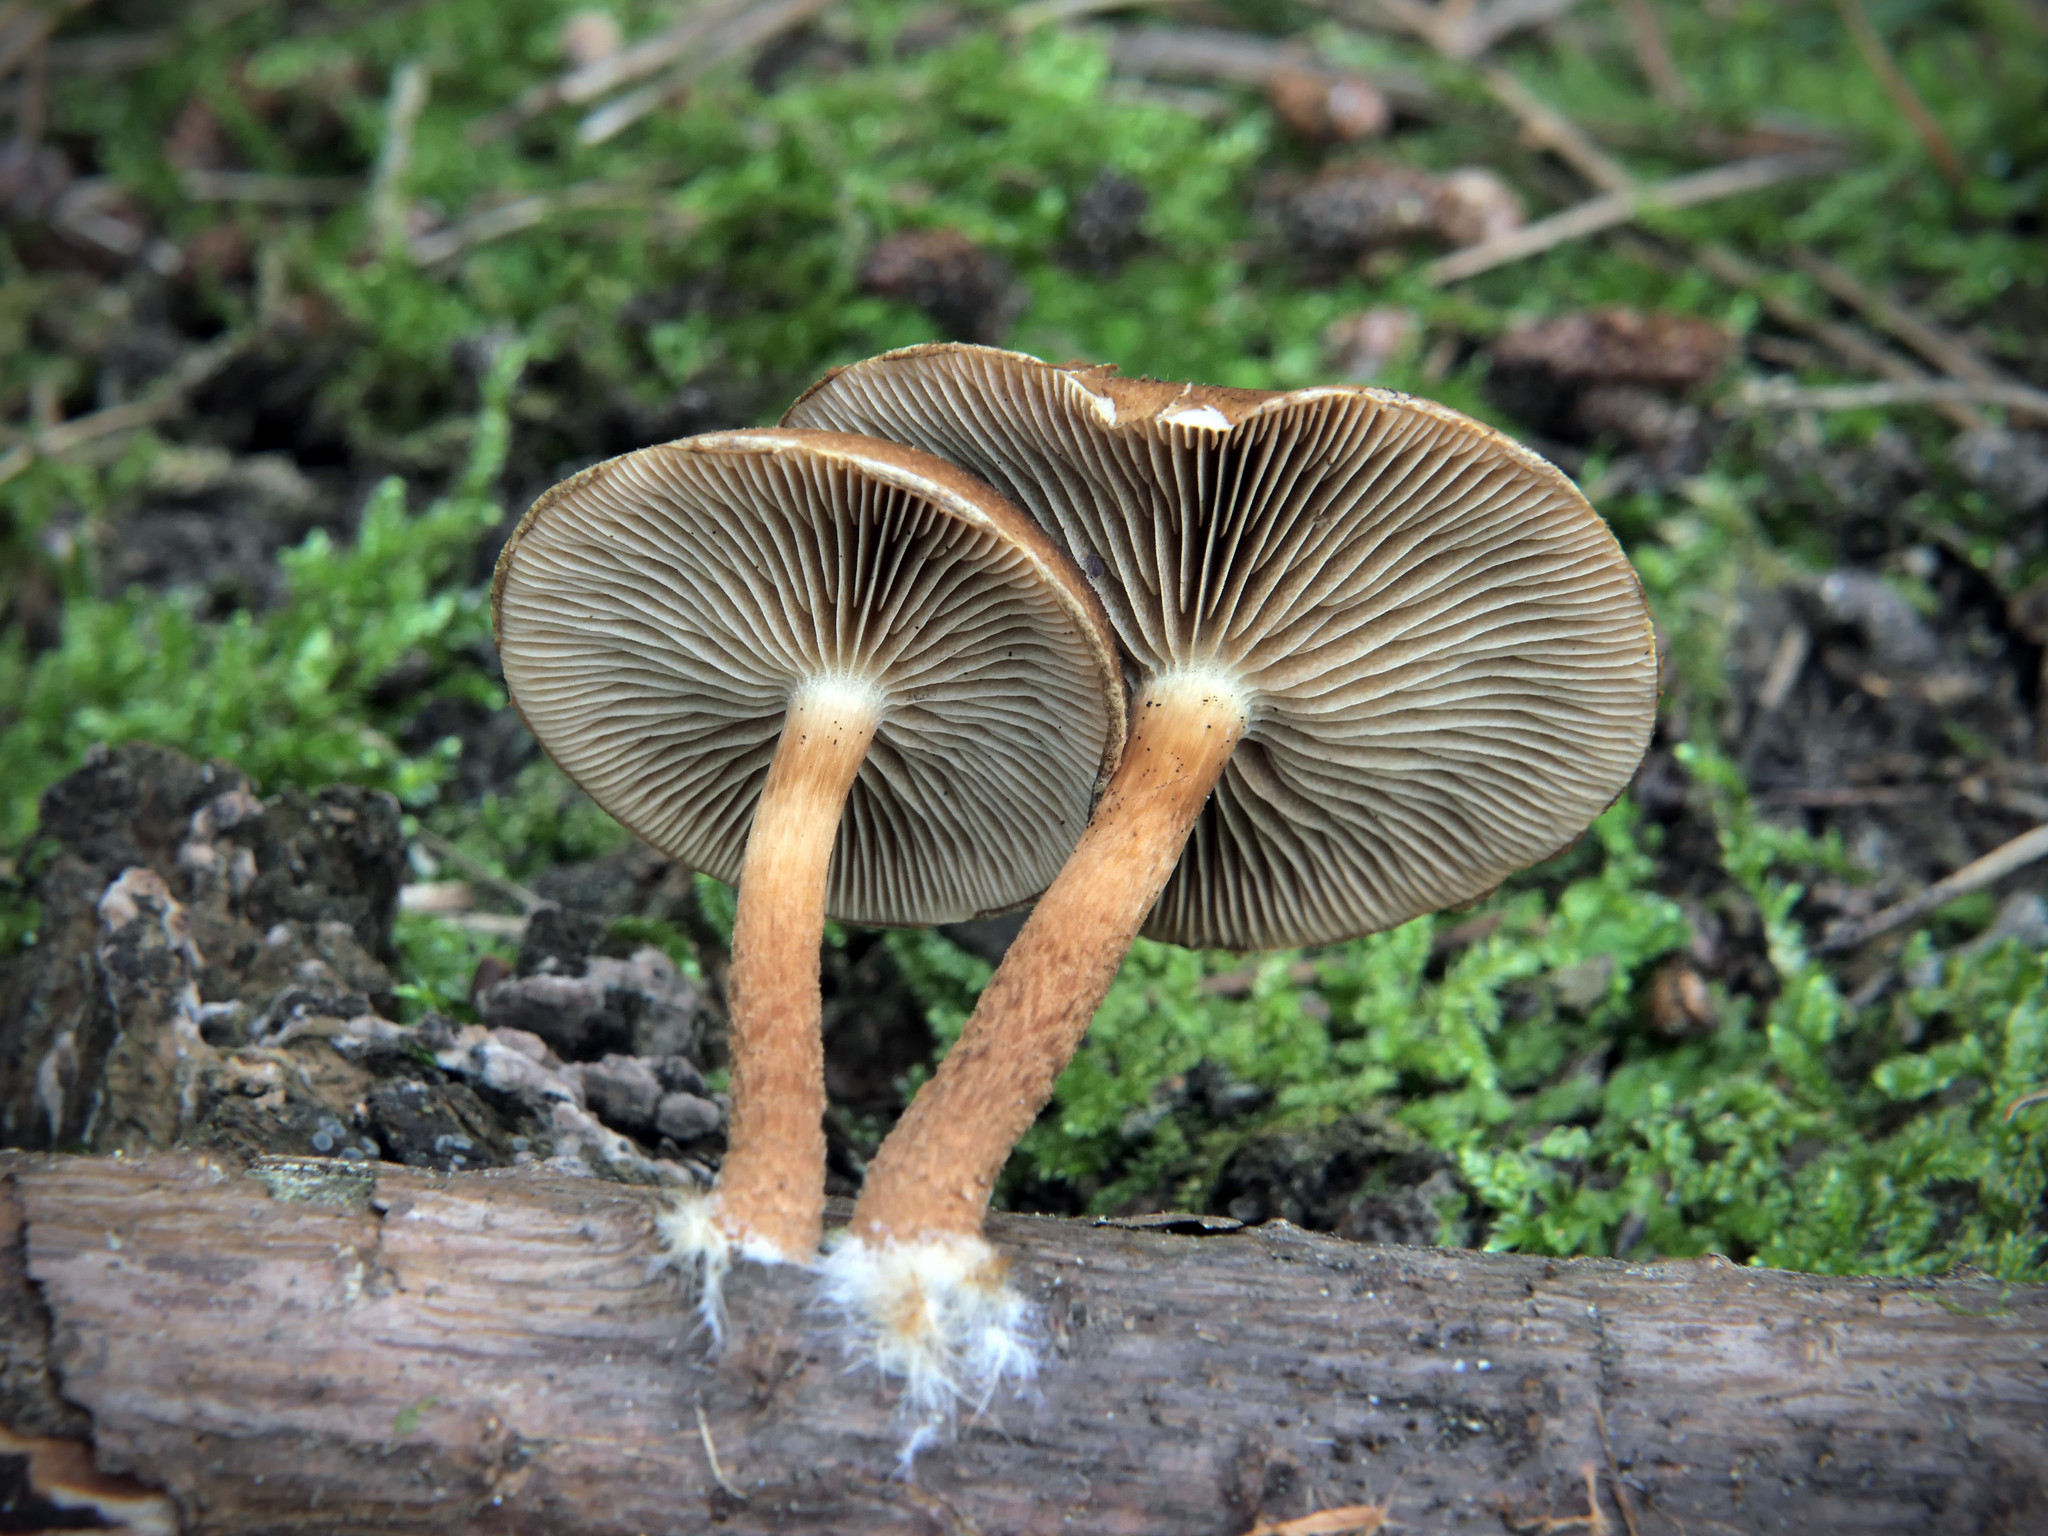
\includegraphics[width=0.45\linewidth ]{figures/02_literature/1.jpg}}
    \hfill
    \subcaptionbox{}{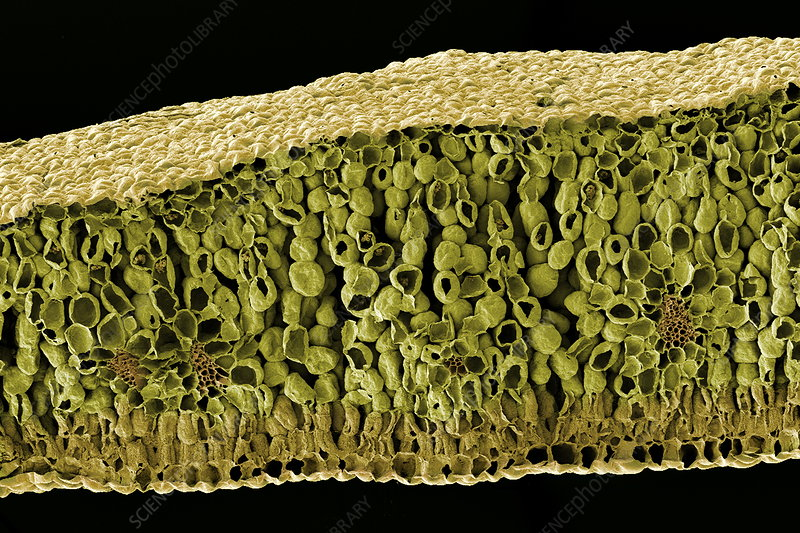
\includegraphics[width=0.45\linewidth ]{figures/02_literature/3.jpg}}
    \bigskip
    \subcaptionbox{}{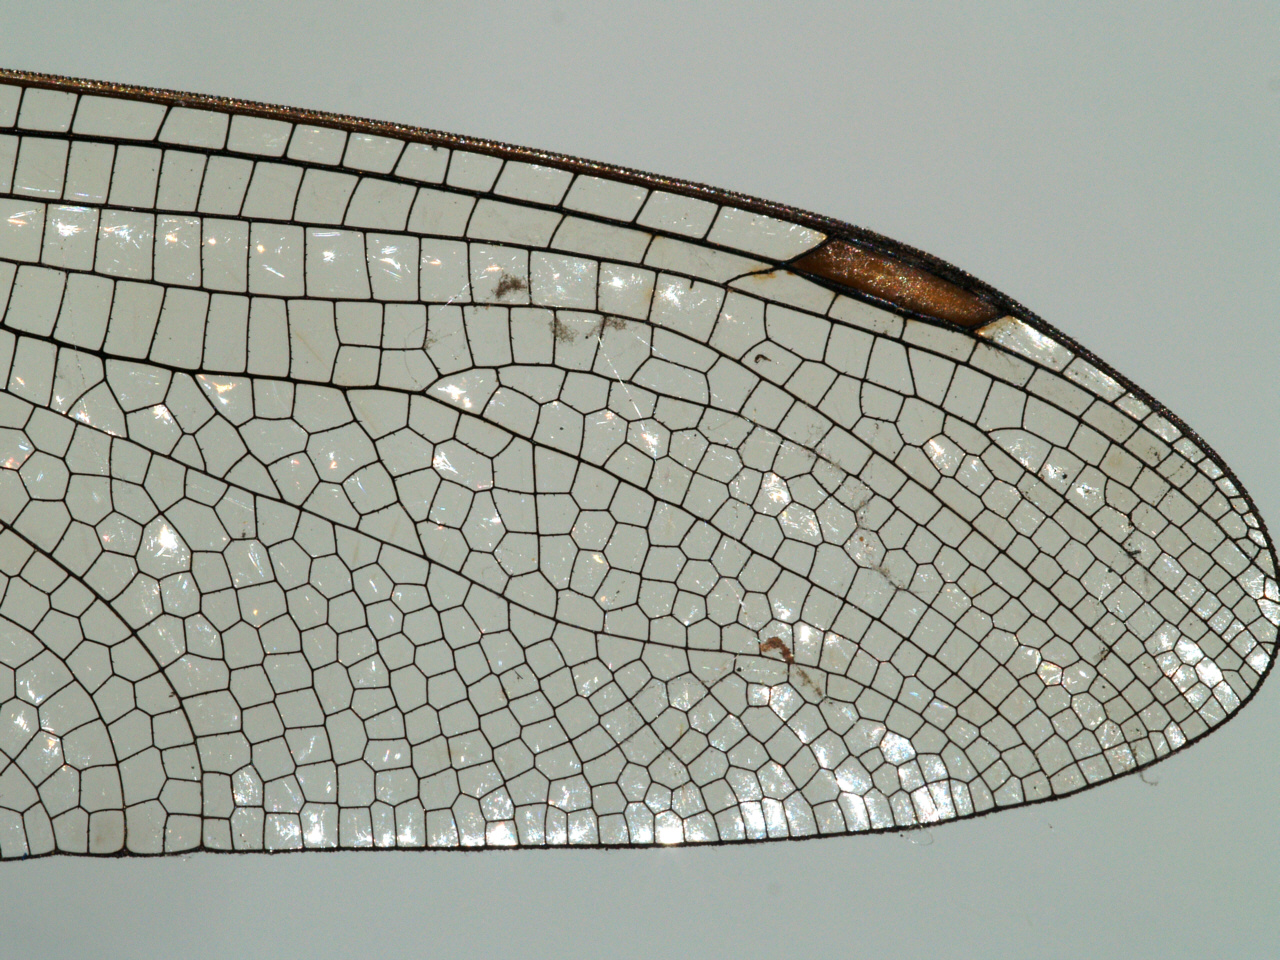
\includegraphics[width=0.45\linewidth ]{figures/02_literature/2.jpg}}
    \hfill
    \subcaptionbox{}{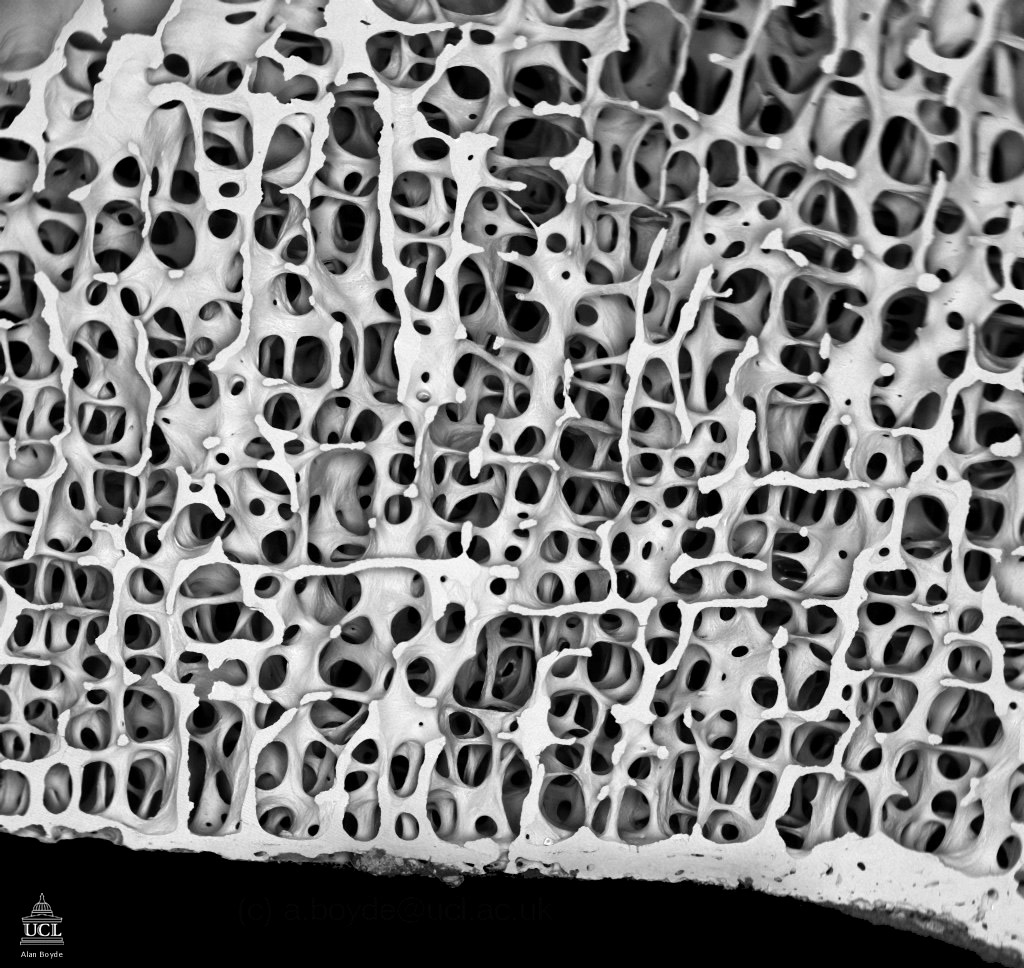
\includegraphics[width=0.45\linewidth ]{figures/02_literature/4.jpg}}
    \caption{The natural evolution process frequently generates lattice materials and modular structures; (a) The spore-bearing gills of a Hypholoma fasciculare \cite{nz_hypholoma_2023}, (b) SEM image of a leaf microstructure \cite{library_leaf_nodate}, (c) architected material of the wing of a dragonfly \cite{gripspix_mostly_off_health_issues_wing_2007}, (d) internal structure of a human bone \cite{noauthor_bone_03_nodate}.}
    \label{fig:02_nature}
\end{figure}

If we observe the Ashby material chart shown in \figref{fig:02_ashby_ch}, where the material yield strength $\sigma_\text{Y}$ is plotted against density $\rho$, it becomes evident that numerous empty spaces exist. Besides some unattainable areas delineated by the \gls{hs} bounds\sidenote{The \gls{hs} bounds are the tightest bounds possible from the range of composite moduli for a two-phase isotropic mixture. In lattices, usually, the second material is void.}, these empty spaces can be filled by lattice materials, extending the property space of actual materials.
\begin{figure}
    \centering
    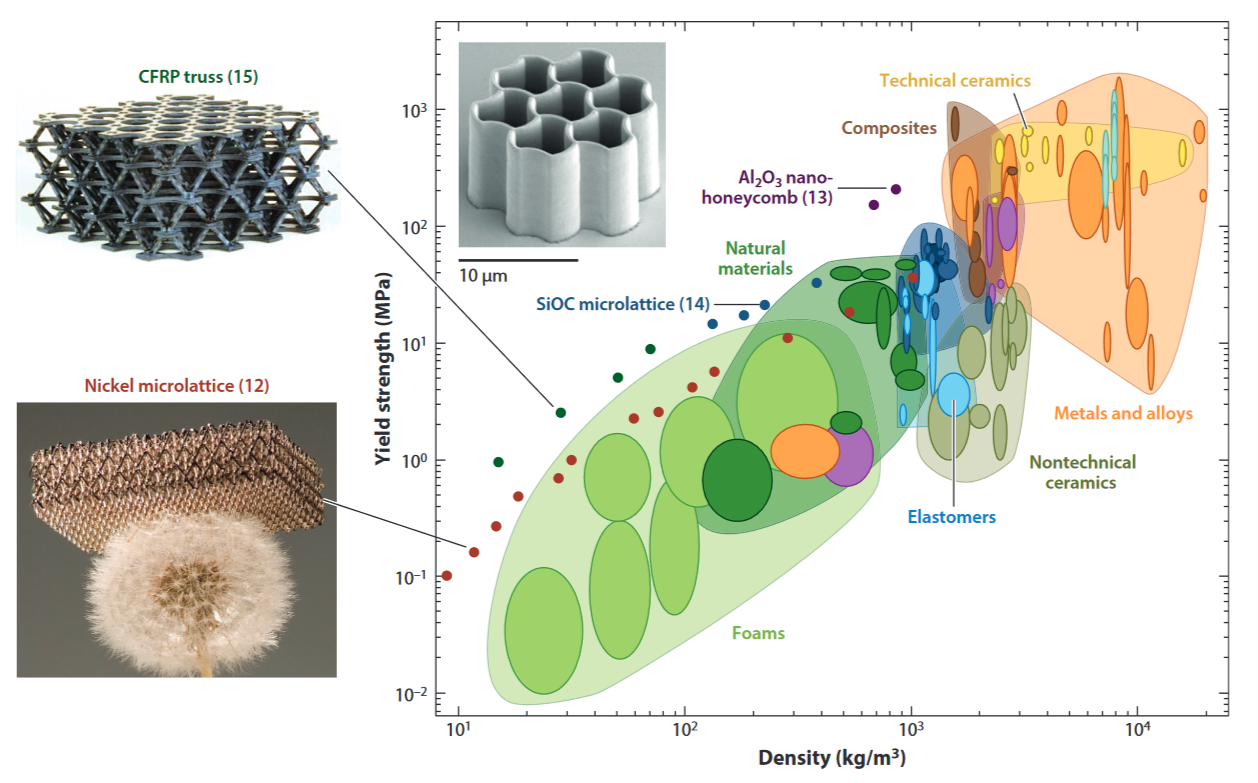
\includegraphics[width=\linewidth]{figures/02_literature/ashby_chart.png}
    \caption{Density versus yield strength Ashby chart. Exploiting the architecture of the material as a variable to design new metamaterials, empty spaces of the graph can be filled (see dots) \cite{schaedler_architected_2016}.}
    \label{fig:02_ashby_ch}
\end{figure}

Up to this point, we discussed materials, implicitly assuming that the bounding volume in which we find the arrangement of solids and voids, called \gls{rve}, is small compared to the macrostructure. However, it is possible to differentiate between a lattice material and a lattice structure exactly based on the size of the \gls{rve} with respect to the considered structure. In a modular lattice structure, there is no clear physical scale separation between the \gls{rve} and the structure, indicating that the \gls{rve} mechanical characteristics are manifested at both the micro and macro scales. However, defining a specific threshold to distinctly categorize the two is challenging, as the transition from lattice material to lattice structure can be gradual and context-dependent~\sidecite{dai_size_2008,kalamkarov_asymptotic_2009,coelho_scale-size_2016,zhang_multiscale_2018}.

Lattices can be categorized as open- or closed-wall based on the topology they show. Despite the use of closed-wall lattices potentially resulting in stiffer structures, the preference for open-cell configurations is well-articulated by Sigmund \etal~\sidecite{sigmund_non-optimality_2016}. They emphasize that the outcome of minimum compliance topology optimization studies should inherently be of sheet type when using density methods unless explicit constraints favoring open-wall structures are specified. These constraints include considerations of structural and microstructural stability, as the load required to initiate buckling in a slender strut of an open-cell lattice is significantly higher than that of a comparable closed-cell lattice~\sidecite{deshpande_foam_2001}. Consequently, open-cell structures are less prone to buckling. Additionally, the porosity of open-wall cells allows for the passage of flow, making them suitable for applications such as heat exchangers or promoting bone regrowth in biomedical scaffolds. From a manufacturing perspective, open-cell designs are preferable, as very thin walls are challenging to manufacture. The transparency inherent in open-cell structures is advantageous for tasks such as repair and health monitoring. Finally, an open-cell design is considered elegant and aesthetic, as it embodies Michell-like structures, which are described as "inarguably beautiful" and "look elegant and efficient" by Sigmund \etal~\cite{sigmund_non-optimality_2016}.
\begin{marginfigure}
    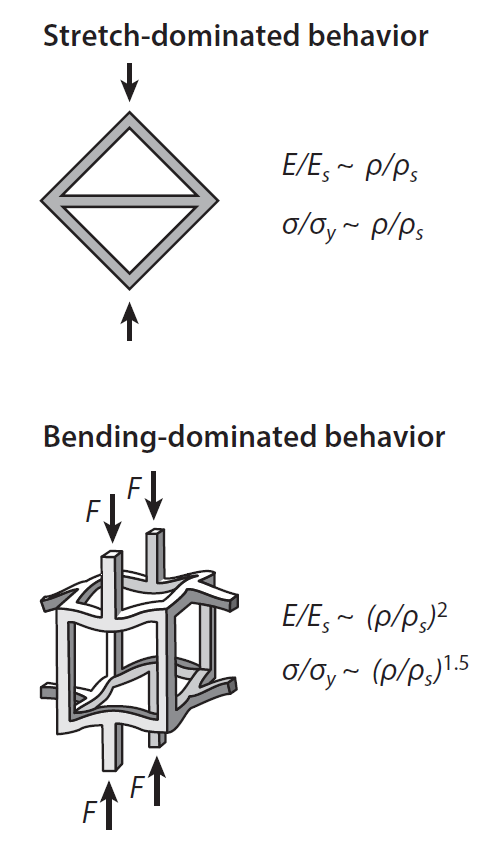
\includegraphics[width=\textwidth]{figures/02_literature/stretc-bend.png}
    \caption{A stretch-dominated and a bending-dominated \gls{rve}. Bending-dominated cells act as a mechanism if the joints cannot withstand moments. The scaling laws are different for the two structural families \cite{schaedler_architected_2016}.}
    \label{fig:02_str_bend}
\end{marginfigure}

Lattices are further categorized into stretching- and bending-dominated based on the failure mode they show when loaded. A stretching-dominated lattice is characterized as a lattice in which its constitutive struts exclusively experience tension and compression loads. In such a structure, the nodal stiffness does not contribute to the overall structural stiffness, and the truss undergoes collapse primarily through the stretching of its struts. Desphande \etal~\cite{deshpande_foam_2001} noted that freezing the joints of a stretching-dominated truss has minimal impact on its macroscopic stiffness or strength. Despite the bending of the struts, the frame remains stretching-dominated, and the collapse load is predominantly determined by the axial strength of the struts. Consequently, if an open-cell lattice is stretching-dominated, it can effectively be treated as a connected set of pin-jointed struts.

The relative density of the lattice is defined as:
\begin{equation}
    \bar{\rho} = \frac{\rho_l}{\rho}
\end{equation}
where $\rho_l$ and $\rho$ represent the density of the lattice and the dense material, respectively~\sidecite{ashby_properties_2006}. A stretching-dominated lattice exhibits approximately 10 times greater stiffness and 3 times greater strength than a bending-dominated lattice at $\bar{\rho} = 0.1$, as illustrated in Figure~\ref{fig:02_str_bend}. Nevertheless, when subjected to compression, stretching-dominated lattices display a softening post-yield response attributed to the buckling of struts, rendering them less suitable for energy absorption tasks. In contrast, bending-dominated lattices showcase a more favorable energy-absorbing behavior, characterized by a plateau-like response. Bending-dominated lattices are often named foams \cite{ashby_properties_2006}.

Lattice structures and materials exhibit a wide range of promising applications. They showcase notable energy-absorbing properties, particularly when designed as being bending-dominated~\sidecite{evans_concepts_2010,schaedler_designing_2014,ozdemir_energy_2016}. This quality positions lattices as potential candidates for novel design schemes in aerodynamics, thanks to their remarkable aeroelastic properties~\sidecite{opgenoord_aeroelastic_2018,cramer_elastic_2019}. Additionally, lattices have proven to be compelling choices for constructing biomedical scaffolds, promoting bone ingrowth~\sidecite{hutmacher_scaffolds_2000,mota_additive_2015,nikolova_recent_2019}. Furthermore, lattice materials demonstrate excellent heat exchanger properties, attributed to their high surface-to-volume ratio and the turbulent mixing flow they induce when a fluid passes through~\sidecite{lu_heat_1998,wadley_thermal_2007}.
\begin{marginfigure}
        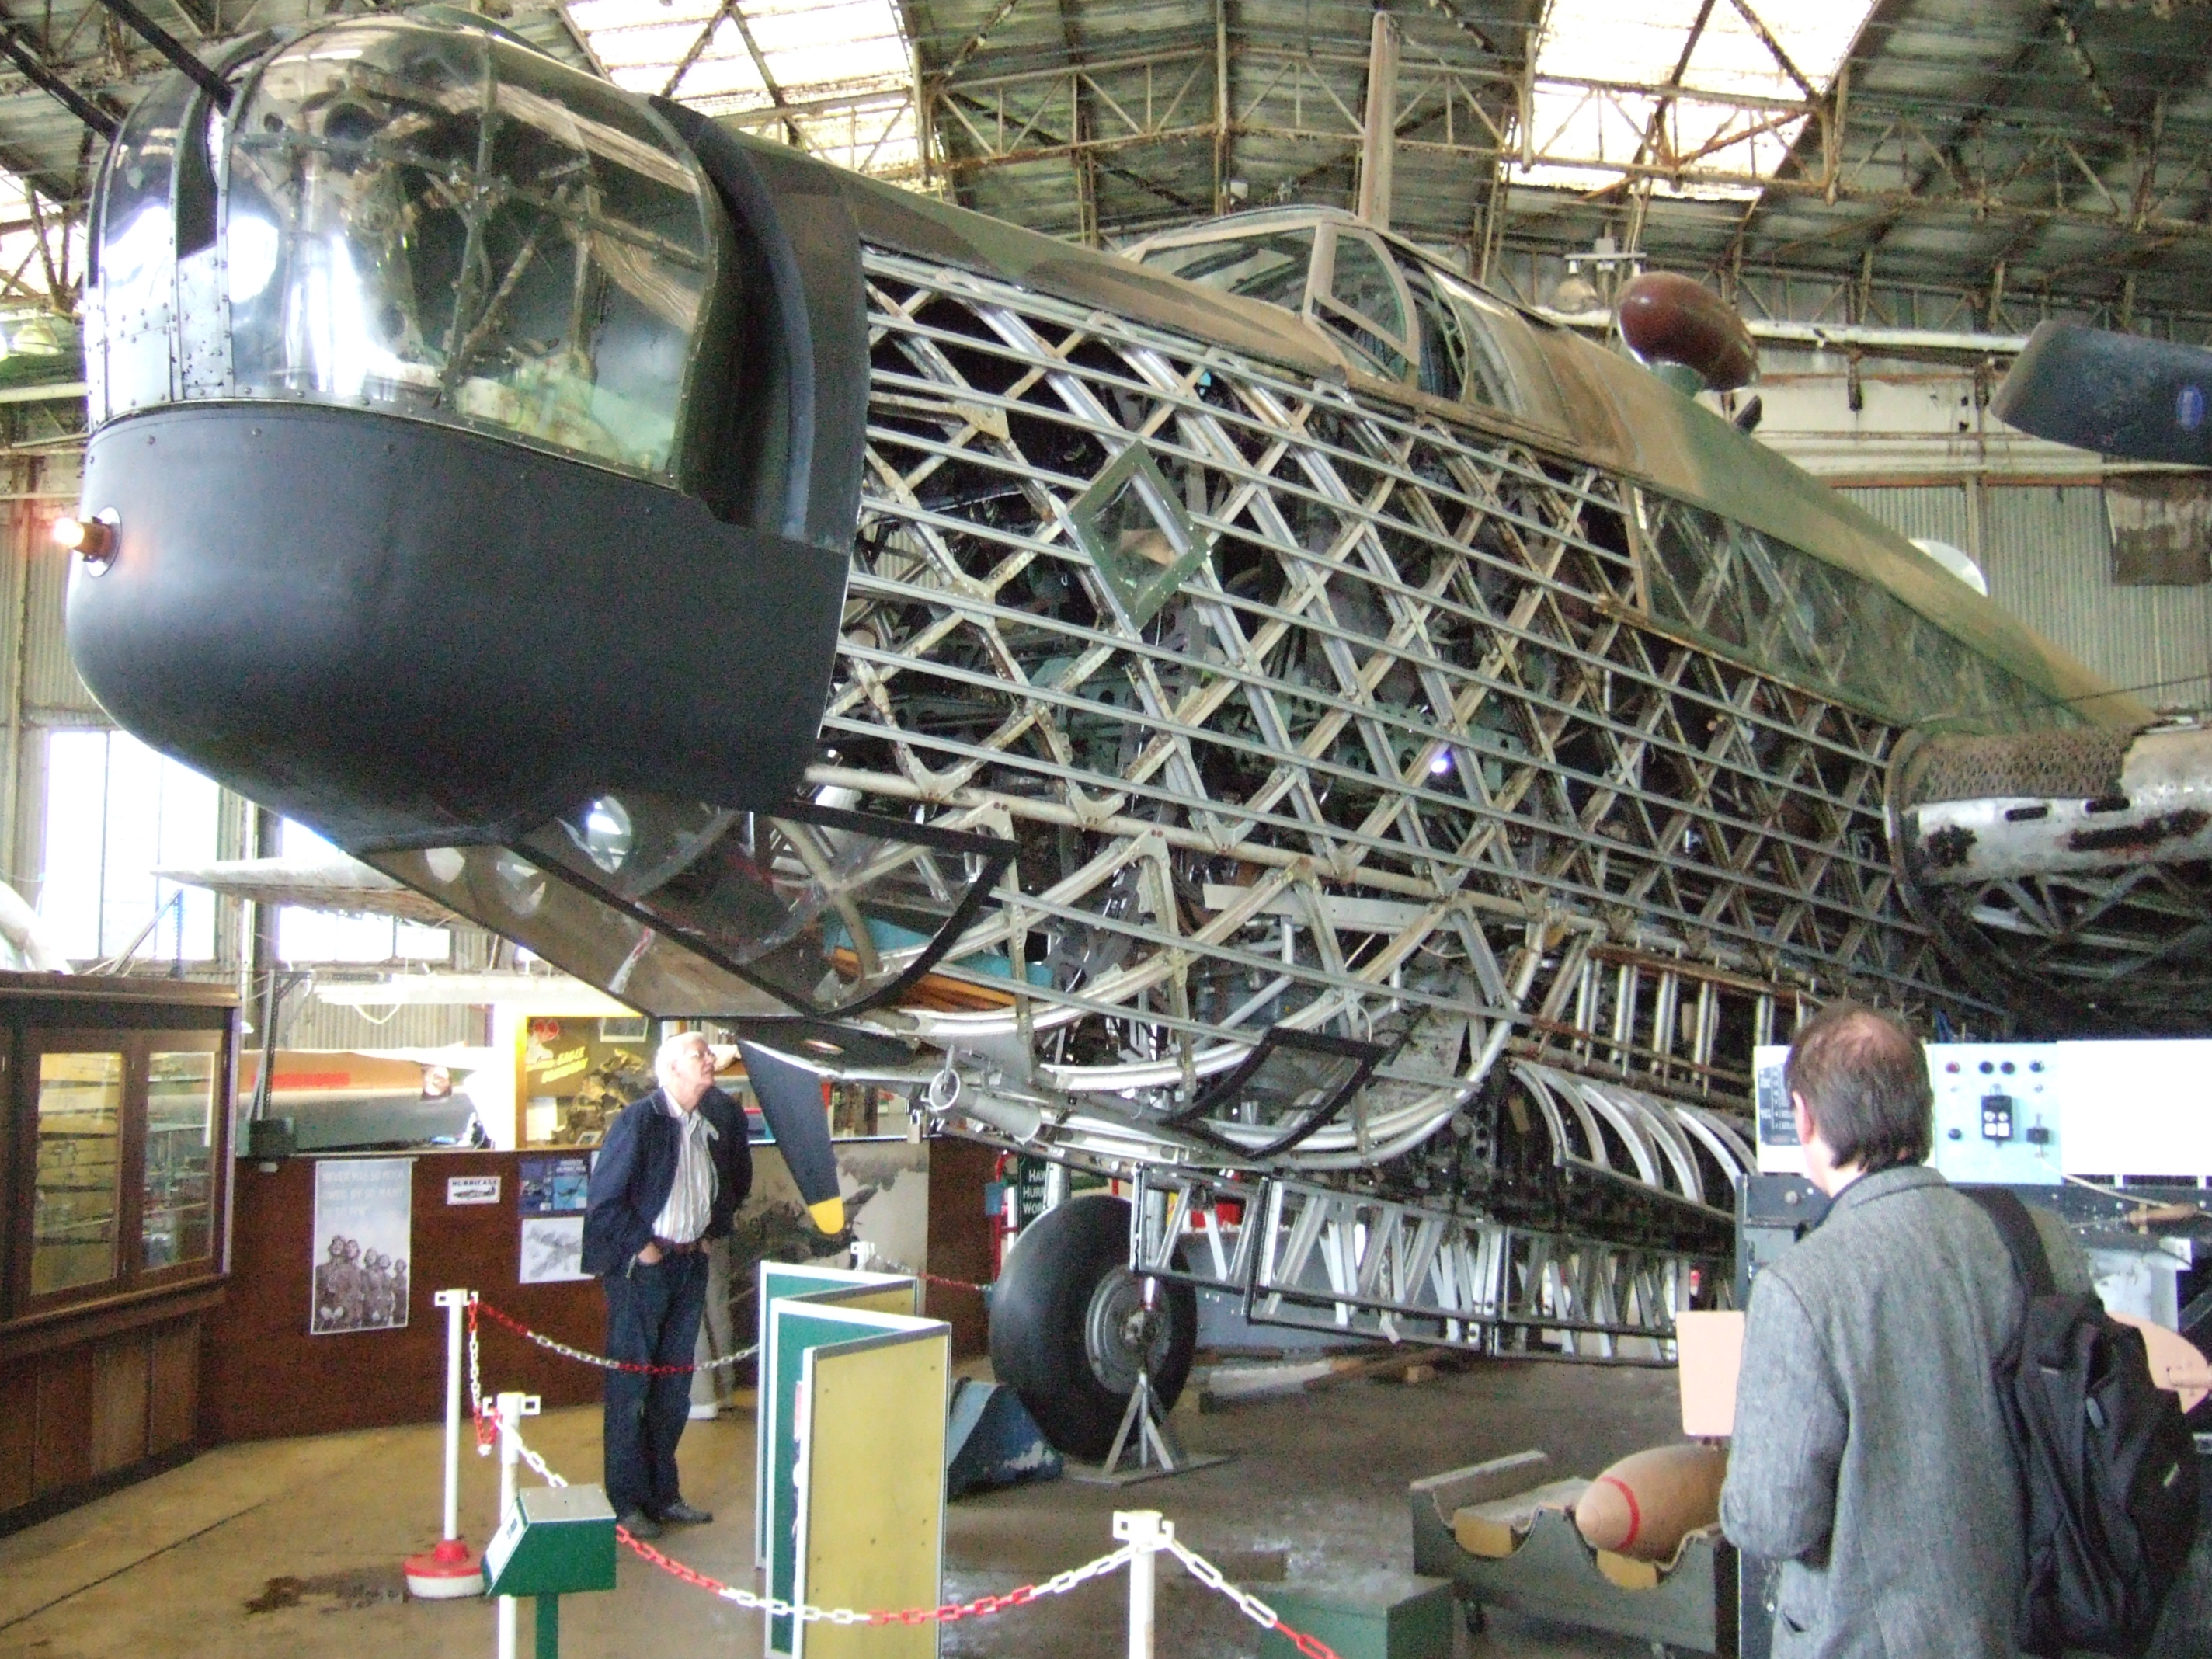
\includegraphics[width=\linewidth]{figures/02_literature/wellington.jpg}
        \caption{Vickers Wellingtons, bombers utilized during World War II, remained operational despite sustaining extensive damage, thanks to their modular fuselage. When one of the ribs was damaged, the load was redistributed to the others, allowing the structure to remain functional \cite{airshowconsultants_real_2013}.}
        \label{fig:vick}
\end{marginfigure}

An interesting class of architected materials is represented by modular lattices, alternatively referred to in the literature as cellular architected materials. The defining feature of lattice materials is to exhibit a repetitive cell (also called module when dealing with lattice structures and not materials) that is replicated throughout space. This characteristic allows for the establishment of a systematic and reproducible unit that captures the essential structural and material properties of the lattice. The study of the repetitive nature of the \gls{rve} \ie, the part of the structural domain that is populated with a cell, permits a comprehensive understanding of the cellular lattice's behavior, enabling researchers to analyze and predict its mechanical, thermal, and other pertinent properties with a high degree of accuracy~\sidecite{bensoussan_asymptotic_1978}. 

Modular structures show additional captivating properties that demonstrate their versatility. Firstly, modular structures can be purposefully designed for reversible assembly, introducing the concept of rapid assembly and easily repairable structures (see \figref{fig:02_madcat}). Various approaches, such as utilizing fasteners~\sidecite{cheung_reversibly_2013,jenett_digital_2017,cramer_elastic_2019}, or incorporating snap-fit joints~\sidecite{dong_mechanical_2015}, have been proposed to realize this idea. Furthermore, modular structures inherently exhibit damage tolerance~\sidecite{stolpe_fail-safe_2019,wu_topology_2021} \eg, in a skin-lattice design, the skin is non-load-bearing, ensuring that skin damage does not lead to progressive structural failure. Additionally, in cases of rib damage, the affected rib can be isolated from the load without compromising the integrity of the entire structure (refer to Fig.~\ref{fig:vick}). Lastly, modular structures pave the way for extensive utilization of robotics in both the manufacturing~\sidecite{hunt_wraptor_2019} and assembly phases~\sidecite{gershenfeld_macrofabrication_2015,jenett_bill-e_2017,costa_algorithmic_2020,niehs_recognition_2020}.
\begin{figure}
    \centering
    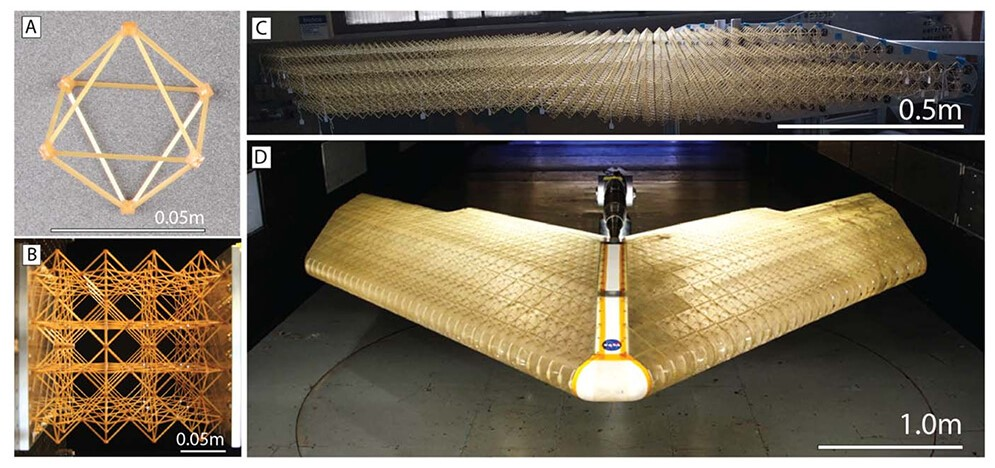
\includegraphics[width=\linewidth]{figures/02_literature/nasa-madcat-morphing-wing-breakdown-1000-x-600(1).jpg}
    \caption{The different length scales present in a lattice structure~\cite{cramer_elastic_2019}. The size of the module (shown in subfigure A) is comparable with the dimensions of the wing, especially in the thickness. We therefore talk about lattice structure and not material.}
    \label{fig:02_madcat}
\end{figure}

There is no consensus on the terminology of lattice materials and structures, leading to confusion with multiple names in the literature. Some define a "cellular structure" as one comprising nodes and struts connecting those nodes, where all struts may have different cross-sectional areas \sidecite{opgenoord_transonic_2018, park_design_2022}. When a cellular structure exhibits a repeating pattern, it is referred to as a "lattice structure". Conversely, others use "cellular" and "lattice" interchangeably when discussing materials and structures that shows a stretch dominqted behaviour \sidecite{deshpande_foam_2001, ashby_properties_2006}. In such cases, the opposite of a lattice material is often termed a "foam" \ie a bending-dominated architected material \cite{deshpande_foam_2001}. Additionally, there is often ambiguity between the terms "material" and "structure," despite their distinct concepts. For example, many works describe lattice structures as RVEs with homogenized mechanical properties \sidecite{xu_design_2016, song_investigation_2021}.

To address these issues, we opted to establish clarity by using different terminology depending on whether we are discussing materials (with scale separation) or structures (without scale separation). This approach helps to eliminate any confusion in this thesis. The chosen terminology is presented in \tabref{tab:02_modular_names}.

\begin{table*}
    \small
    \centering
    \begin{tabular}{
        y{6cm}
        x{3.5cm}
        x{3.5cm}}
        \toprule
        \textbf{Description} & \textbf{Material {(Scale separation)}} & \textbf{Structure {(No scale separation)}} \\ \midrule
        Whole domain & Macrostructure & Structure \\\addlinespace[2mm]
        Properties are dictated by the spacial arrangement of voids and solids & Lattice, architected  & Lattice, architected \\\addlinespace[2mm]
        Properties are dictated by the stochastic spacial arrangement of voids and solids &Cellular&Modular\\\addlinespace[2mm]
        Repetitive entity & Cell, microstructure & Module \\\addlinespace[2mm]
        Part of the domain where the repetitive entity is placed & RVE & Subdomain \\
         \bottomrule
    \end{tabular}
    \caption{Vocabulary used in this document to write about lattice materials and modular structures. The adjectives architected and lattice are the only one that are used for both materials and structures.}
    \label{tab:02_modular_names}
\end{table*}

\subsection{Modular structures and cellular materials optimization}
The initial density-based topology optimization method, as seen in Bendsøe and Kikuchi's foundational work~\sidecite{bendsoe_generating_1988}, employed numerical homogenization to model a meta-material consisting of infinitesimally small square cells with square holes. Notably, this marked the advent of multi-scale optimization, driven by the observation that optimal stiffness for a structure encompasses various scales \sidecite{kohn_optimal_1986,allaire_optimal_1999}.

In the 1990s, the focus shifted from homogenization algorithms to mono-scale algorithms, where the optimization involved a homogeneous distribution of an isotropic material \sidecite{bendsoe_optimal_1989,zhou_coc_1991}. This shift was primarily caused by the manufacturing challenges associated with producing multi-scale meta-materials. Subsequently, these approaches evolved into what is now known as density-based topology optimization. Mono-scale methods, where the design domain discretization results in structures at a single scale, can achieve theoretical stiffness-optimal structures spanning multiple scales with fine mesh discretization and careful continuation techniques. Bendsøe and Kikuchi's original work and homogenization-based algorithms have gained recently more interest due to the advances in additive manufacturing technologies. Contemporary studies are combining asymptotic homogenization and topology optimization to optimize multi-scale structures. 

Modular structures and cellular materials are optimized through either a multi-scale or a full-scale approach. Multi-scale algorithms operate on structures with different physical scales between the micro- and macro-levels, assuming periodic boundary conditions for the \gls{rve}. Doing that allows for the use of a material model with micro-structure properties evaluated using asymptotic homogenization. In contrast, full-scale methods represent mono-scale approaches where modular optimization is achieved by controlling the layout locally. In these full-scale approaches, both analysis and optimization are conducted at the full resolution of the domain. For a more in-depth exploration and comparison of full-scale and multi-scale approaches, interested readers can refer to the comprehensive review by Wu \etal \sidecite{wu_topology_2021}.

\subsection{Multi-scale structures optimization}
Optimal structures span multiple scales, and using a finer mesh allows for detailed geometric improvements, potentially enhancing optimized structures. However, higher-resolution mono-scale approaches come with increased computational costs. To tackle this, multi-scale approaches like the hierarchical method by Rodrigues \etal~\sidecite{rodrigues_hierarchical_2002} and de-homogenization techniques~\sidecite{pantz_post-treatment_2008, groen_homogenization-based_2018} have been introduced.

The hierarchical optimization framework consists of a master problem addressing the global spatial distribution of material and an inner problem tackling the optimal choice of material at the local level. This approach shifts the focus from a specific composite's material distribution problem to a more comprehensive challenge involving both topology and material optimal design. The idea is to use the homogenized microscale cell as the base material of the macroscale topology optimization. \figref{fig:02_homogen} gives a graphical representation of how asymptotic homogenization works.
\begin{figure}
    \centering
    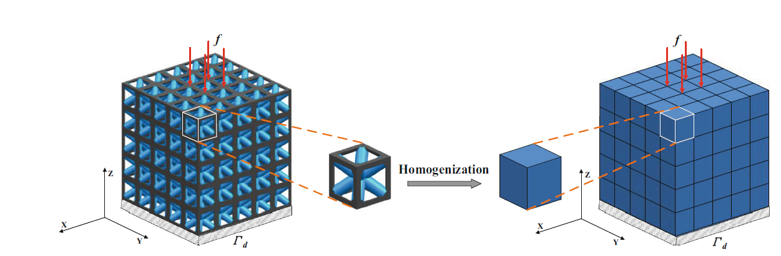
\includegraphics[width=\linewidth]{figures/02_literature/homo.png}
    \caption{Graphical representation of the asymptotic homogenization method used to retrieve the equivalent mechanical properties of a periodic cell \cite{wang_concurrent_2020}.}
    \label{fig:02_homogen}
\end{figure}
The equivalent elastic tensor $\mathbf{C}^{H}$ is calculated using the following formula~\sidecite{guedes_preprocessing_1990}:
\begin{equation}
    \mathbf{C}^{H}=\frac{1}{\left|\Omega_{m}\right|} \int_{\Omega_{m}} \left(\varepsilon_{m}^{0}-\varepsilon_{m}\right)\mathbf{C}\left(\varepsilon_{m}^{0}-\varepsilon_{m}\right) d \Omega_{m}
\end{equation}
where $\Omega_{m}$ represents the \gls{rve} volume, $\mathbf{C}$ is the base material elastic tensor and $\boldsymbol{\varepsilon}_{m}^{0}$ are called unit test strain and are defined as $\boldsymbol{\varepsilon}^{11}=(1,0,0)^{T}, \boldsymbol{\varepsilon}^{22}=(0,1,0)^{T}, \boldsymbol{\varepsilon}^{12}=(0,0,1)^{T}$. An example of the results obtained using a hierarchical method is presented in \figref{fig:02_hierarchical}.
\begin{figure}
    \centering
    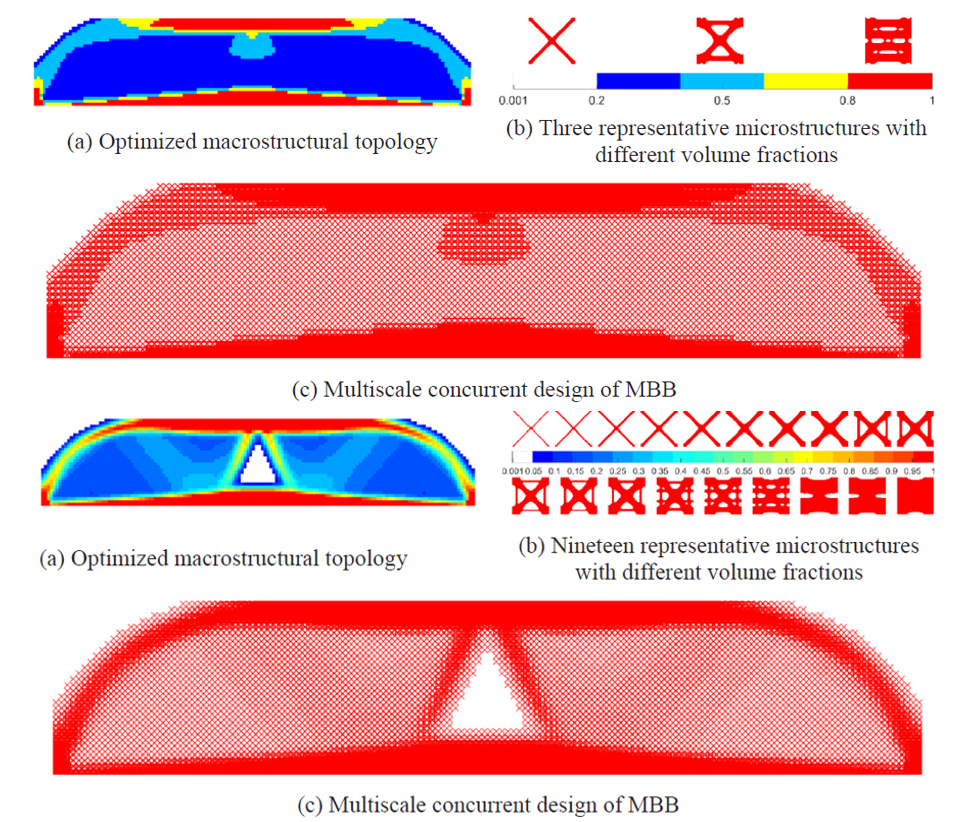
\includegraphics[width=0.9\linewidth]{figures/02_literature/top_multiscale.png}
    \caption{In the study of Zhang \etal \cite{zhang_multiscale_2018} the same test case is optimized using a hierarchical optimization method and a different number of microstructures. Here we show the multi-scale optimized structures using 3 and 19 different microstructures. The structure with 19 microstructures is \qty{10}{\percent} stiffer compared to the one with 3.}
    \label{fig:02_hierarchical}
\end{figure}

De-homogenization is an approach where the optimization problem is initially solved solely on the macroscopic level using a homogenization method. Subsequently, an additional phase is introduced to obtain connected and physically realizable microstructures based on the obtained macroscopic result. In the macroscale optimization, multiple additional parameters are typically optimized concurrently with the density of the \gls{rve}. These parameters may include microstructure orientation, contributing to the creation of a smooth mapping function \sidecite{groen_homogenization-based_2018,allaire_topology_2019,geoffroy-donders_3-d_2020,kumar_density-and-strain-based_2020}. An alternative approach involves approximating the material behavior through a reduced database model, as demonstrated by Xia and Breitkopf \sidecite{xia_multiscale_2015}. In this method, microstructural computations are performed offline, only once, to reduce the computational time of successive optimizations. Precomputed databases are often employed to obtain the full design for the parametrized lattice \gls{rve}, often using a polynomial model to interpolate between the database microstructures \sidecite{wang_concurrent_2018,imediegwu_multiscale_2019,duriez_well_2021}. Recent approaches are now using \gls{ai} and deep learning to speed up the de-homogenization phase~\sidecite{kim_machine_2021,white_multiscale_2019,chandrasekhar_multi-material_2021,wang_enhancing_2021} 

In conclusion, despite maintaining the separation of the two physical scales during the optimization process, it is imperative to conduct a full-scale validation for all multi-scale methods, as highlighted in various studies \sidecite{groen_homogenization-based_2018,wu_topology_2021, duriez_well_2021, sigmund_benchmarking_2022}. Additionally, the multi-scale optimization approaches in which the microstructure is aligned to local stress fields without constraints imposed by cell geometry or orientation \cite{groen_homogenization-based_2018}, deliver good performance even for structures with less periodicity compared to a bulk distribution.

\subsection{Full-scale structures optimization}
\begin{figure*}
    \centering
    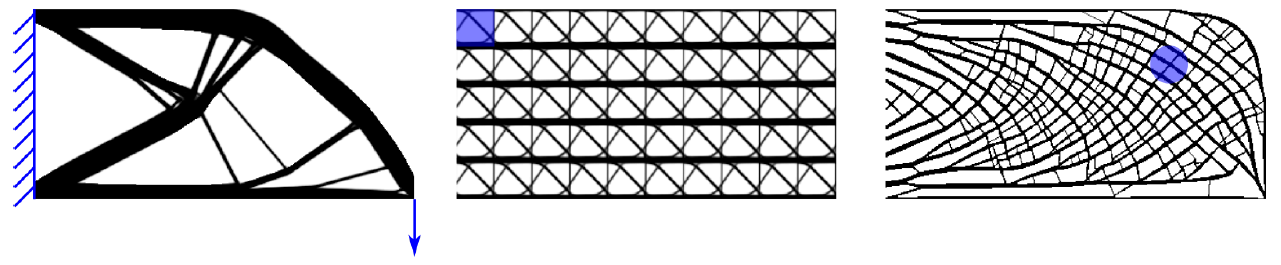
\includegraphics[width=0.8\linewidth]{figures/02_literature/full-to.png}
    \caption{Three structures with the same volume are optimized for compliance minimization using three different methods: on the left, a classic mono-scale topology optimization algorithm. Middle: the variable linking method is used to enforce the pattern repetition on the structure. On the right an optimized structure with local volume constraints. The algorithms used to optimize the last two structures belong to the family of \textit{full-scale} methods. \cite{wu_topology_2021}.}
    \label{fig:02_full-to}
\end{figure*}

Recent studies have focused on assessing homogenization predictions compared to mechanical responses, revealing up to a \qty{20}{\percent} variation in the effective components of the stiffness tensor for a $6\times6\times6$ cube when compared to homogenized models \sidecite{coelho_scale-size_2016,cheng_functionally_2019}. This variability is attributed to the "boundary layer phenomenon" observed in the late 70s, challenging the assumptions of periodic boundary conditions and scale separability inherent in homogenization \sidecite{bensoussan_asymptotic_1978,kalamkarov_asymptotic_2009}. To address these limitations, a new family of methodologies, known as full-scale approaches, has emerged. Unlike homogenization-based methods, full-scale approaches, such as pattern repetition (also known as variable linking) and local volume constraints, avoid reliance on homogenization. In pattern repetition, the initial design space is partitioned into repetitive domains that are optimized and constrained to ensure their uniformity \sidecite{zhang_scale-related_2006}. In contrast, the local volume constraints method imposes an upper limit on the solid elements' fraction in a neighborhood radius centered at each point within the design domain. The objective is to generate porous structures aligned with principal stress directions. While experiencing a modest stiffness reduction compared to mono-scale designs, these structures demonstrate heightened resilience against variations in load angle, local material failure, and buckling \sidecite{wu_infill_2018}.

Variable linking approach faces a common limitation, leading to compromised structural performance due to topological periodicity~\sidecite{zhang_scale-related_2006,huang_optimal_2008}. This limitation arises as the design converges toward solutions influenced by the region with the highest compliance, resulting in suboptimal solutions for other regions where the same module design is applied~\sidecite{tugilimana_integrated_2019}. To address this, Bakker~\sidecite{bakker_simultaneous_2021} identified two key approaches. The first involves extending the solution space by introducing additional module properties as design variables. For instance, allowing module rotations has proven effective, as it modifies the local material distribution and enhances structural performance~\sidecite{tugilimana_spatial_2017}. Another possibility would be the use of multiple modules, permitting the subdomains to show a topology tailored to their loading condition \sidecite{tugilimana_integrated_2019,liu_layout_2023}. The second approach involves allowing the module unit to resize, providing flexibility in adapting to different regions within the global domain~\sidecite{stromberg_application_2011,wu_system_2016}. These strategies offer ways to overcome the challenges associated with topological periodicity and achieve more optimized solutions for diverse regions within the structure.

% \setchapterpreamble[u]{\margintoc}
\glsresetall % reset glossary
\chapter{Evaluating discretization approaches for ultralight structure optimization}
The process of topology optimization for a structure involves the selection and sizing of optimal elements within a predetermined set. As discussed in the previous chapter, in our context this set could be composed of either continuum elements (shell or volumetric) or truss-like elements. This chapter aims to assess the suitability and the inherent advantages and disadvantages of both methodologies when optimizing ultralight structures \ie structures that exhibit \marginnote{Part of the content presented in this chapter has been published and showcased during a conference as:\\Stragiotti, E. et al. (2021) "Towards manufactured lattice structures: a comparison between layout and topology optimization", in \textit{AeroBest 2021 International Conference on Multidisciplinary Design Optimization of Aerospace Systems}. Book of proceedings. Lisbon, Portugal: ECCOMAS~\cite{stragiotti_towards_2021}.} an extremely low volume fraction, typically below 1\%. 

For this purpose, we initially establish a common optimization formulation in \secref{sec:03_common_prob}. The classic compliance minimization with volume constraint problem is reformulated as a volume minimization problem with maximum stress constraints for both discretizations. Later, this framework is applied to optimize a two-dimensional test case, featuring identical dimensions, loads, and material properties. The outcomes of the comparison of both discretization approaches are presented and discussed in \secref{sec:03_comparison}. 

\section{The formulation of a common problem: volume minimization with stress constraints} \label{sec:03_common_prob}
Two of the most frequently employed formulations for structural optimization are the minimization of volume while adhering to stress constraints and the minimization of compliance under volume constraints. Historically, the volume minimization formulation has been used in the first works of structural optimization of truss structures~\sidecite{dorn_automatic_1964,chan_optimum_1964,hemp_optimum_1973}. The problem was initially formulated in terms of member forces, ignoring the kinematic compatibility to obtain a \gls{lp} problem. The formulation was modeled using the \acrfull{sand} approach, where the equations of nodal equilibrium are treated as equality constraints, and where both nodal displacements and the cross-sectional areas of truss members serve as design variables~\sidecite{sankaranarayanan_truss_1994}. 

However, to attain greater design freedom, the structure optimization field later transitioned from truss structures to continuous discretization. While truss structures offered simplicity and ease of analysis, they imposed limitations on design due to their discrete member configurations. The continuum mesh offered instead more versatility~\sidecite{bendsoe_generating_1988,bendsoe_optimal_1989}, and has since been used for multiple different applications, \eg the design of metamaterials~\sidecite{sigmund_materials_1994, zhang_scale-related_2006} or the simulation of advanced manufacturing constaints~\sidecite{sigmund_manufacturing_2009,brackett_topology_2011}. The \gls{sand} approach is incompatible with continuum meshes due to its excessive number of variables\sidenote{This preposition holds when referring to the end of the 1980s when computational power was scarce compared to what we have today.}. Given this limitation, a new approach was required to better handle the complexity of continuum meshes.

In the \acrfull{nand} approach, the nodal displacement (state) variables are eliminated from the optimization problem through a process where the structural equilibrium equation is solved every iteration instead of being used as a constraint of the optimization. This results in an independent nested phase where the state equation of structural equilibrium is solved separately from the optimization algorithm. This creates a dense coupling between displacement and material density variables, necessitating a computationally expensive sensitivity analysis within the nested algorithm, typically employing the adjoint method (more information about the adjoint method on the following resurces~\sidecite{tortorelli_design_1994,martins_engineering_2021}). Nevertheless, if the problem is reformulated as a compliance minimization with volume constraints, the problem is self-adjoint and the adjoint algorithm is no longer necessary to evaluate the gradient sensitivities~\sidecite{bendsoe_topology_2004}.

However, our emphasis on operating within the aerospace sector aligns more favorably with the volume minimization problem. The choice to prioritize volume minimization in the aerospace sector is underpinned by a range of economic, environmental, and performance-related factors. It is a strategic approach that aligns with industry goals of sustainability, efficiency, and technological advancement. Additionally, as we will see later in this thesis, the volume minimization formulation will permit adding local buckling and maximum displacement constraints more easily. We have opted, thus, to employ the volume minimization optimization formulation for our study, and we will now review how this formulation is implemented on continuum and truss-like meshes.

\subsection{Continuous discretization \gls{nand} minimum volume formulation}
This section introduces the \gls{nand} volume minimization formulation of topology optimization for continuum meshes. We will start however presenting the more common minimum compliance formulation to explain the important notations and concepts that will be essential in developing the volume minimization formulation.

\paragraph{Minimum compliance formulation}
\begin{marginfigure}
    \centering
    \includegraphics{figures/03_comparison_TO_TTO/01_contin_mesh/c_mesh.pdf}
    \caption{The domain $\Omega$ is discretized using $N_\text{e}=N_\text{x} N_\text{y}$ continuous 4-nodes elements.}
    \label{fig:03_mesh_c}
\end{marginfigure}
Let $\Omega \in \mathbb{R}^2$ be a rectangular domain in of dimensions $X$ and $Y$, containing respectively $N_\text{x}$ and $N_\text{y}$ linear 4-nodes elements, for a total of $N_\text{e}=N_\text{x} N_\text{y}$ elements and $M$ nodes (see \figref{fig:03_mesh_c}). The objective of the optimization is the minimization of the compliance $C$ of the structure, equivalent to finding the structure with the least possible nodal displacement with respect to a defined set of boundary conditions. The Problem $\mathbb{T}_0$ is stated in terms of the design variables $\vect{\rho}$ as follows:
\begin{equation}
    \begin{aligned}
    \min_{\vect{\rho}}         && C &= \sum_{i} \vect{u}_{e,i}^T \matr{K}_{e,i} \vect{u}_{e,i}=\vect{f}^T\vect{u}&& \forall i \in [0,\dots,N_\text{e}]                         \\
    \textrm{s.t.}   && & \frac{\sum_{i} \left(\rhophys_i v_i \right) / V_0}{V_\text{p}} - 1 \leq 0 && \forall i \in [0,\dots,N_\text{e}] \\
    && \matr{K}\vect{u} &= \vect{f} &&\\
    && 0 &\leq \rho_i \leq 1. && \forall i \in [0,\dots,N_\text{e}] \\
    \end{aligned}
    \tag{$\mathbb{T}_0$}
    \label{eq:03_prob-comp}
\end{equation}
The design variables $\vect{\rho}$ are defined for every element of the structure as $\vect{\rho} = [\rho_1, \rho_2, \ldots,\rho_{Ne}]^T$, with $\rho_i \in [0,1], \; \forall i \in [0,\dots,N_\text{e}]$. The physical densities $\vect{\rhophys}$ are related to design variables through density filtering and threshold projection~\sidecite{wang_projection_2011}, as explained later in the document. $V_\text{p}$ is the prescribed volume fraction that acts as the constraint of the minimization problem, while $v_i$ represents the area of the $i$-th element and $V_0$ is the total area of the domain $\Omega$. $\matr{K}\vect{u} = \vect{f}$ is the state equation of the problem and defines the elastic response of the structure to an external nodal load $\vect{f}=[f_1, f_2, \ldots,f_{2M}]^T$. The global stiffness matrix $\matr{K}$ is assembled from the element stiffness matrix $\matr{K} = \sum_{i \in \Omega} \matr{K}_{e,i}$ and $\matr{K}_{e,i} = E_i \matr{K}_{e,0}$ where $\matr{K}_{e,0}$ represents the element stiffness matrix relative to the chosen type of element (linear or quadratic) and $E_i(\rhophys_i)$ the Young's modulus of the $i$-th element. 

The material scheme used to interpolate between void and full material is the well-known \gls{simp}~\sideciteonce{bendsoe_optimal_1989,bendsoe_material_1999} approach. It is governed by the equation:
\begin{equation}
    E_i(\rhophys_i) = E_{\textrm{min}} + \rhophys_i^p(E_0-E_{\textrm{min}}),
    \label{eq:03_simp}
\end{equation}
where the parameter $p$ penalizes the intermediate densities and pushes the result to a black-and-white result. $E_0$ is the Young's modulus of the dense material and $E_{\textrm{min}}$ is a small value used to avoid the global stiffness matrix $\matr{K}$ from being singular when $\rhophys_i=0$. 

In this study we set these parameters to $E_0 = 1$, and $E_{\textrm{min}} = 10^{-9}$. The value of the penalization parameter $p$ is selected as $p=3$ because in that way the intermediate densities respect the \gls{hs} bounds~\sideciteonce{hashin_variational_1963,bendsoe_material_1999}. These relationships describe the boundaries of attainable isotropic material characteristics when dealing with composites (materials with microscopic structures) using two specified, linearly elastic, isotropic materials (in our case the solid and the empty phases).
\paragraph{Spatial filtering and projection}
Multiple approaches have been developed to solve the problems linked to mesh discretization, such as mesh dependence or the checkerboard problem~\sidecite{diaz_checkerboard_1995}. Filtering the sensitivity information of the optimization problem proved to be an effective approach to guarantee independence from mesh resolution~\sidecite{sigmund_design_1994,
sigmund_design_1997}. In the present research, we decided instead to directly filter the density field $\vect{\rho}$ using the 2D convolution operator~\sidecite{sigmund_morphology-based_2007}. The weight function $w$ (or kernel) of the convolution is defined as:
\begin{equation}
    w(d_j) = R - d_j, \quad j \in \mathbb{N}_{i,R}
\end{equation} 
where $\mathbb{N}_{i,R}$ represent the set of elements lying within a circle of radius $R$ centered on the $i$-th element and $d_j$ is the distance of the $j$-th element to the center of the filter (see \figref{fig:03_ker}).
\begin{marginfigure}
    \centering
    \includegraphics{figures/03_comparison_TO_TTO/02_circ_filter/filt_cir.pdf}
    \caption{Kernel of the 2D convolution operator.}
    \label{fig:03_ker}
\end{marginfigure} 
The filtered values of the design variable are calculated as:
\begin{equation}
    \rhofil_i = \frac{\sum_{j \in \mathbb{N}_{i,R}} w(d_j)v_j\rho_j}{\sum_{j \in \mathbb{N}_{i,R}} w(d_j)v_j}.
    \label{eq:03_rhofil}
\end{equation}
As the filtering phase produces a large number of gray elements, a smooth projection technique based on the \textit{tanh} function is implemented~\sidecite{wang_projection_2011}:
\begin{equation}
    \rhophys_j = \frac{\tanh(\beta\eta)+\tanh(\beta(\rhofil_j - \eta))}{\tanh(\beta\eta)+\tanh(\beta(1 - \eta))},
    \label{eq:03_proj}
\end{equation}
where $\beta$ is a parameter that defines the slope of this approximation function: the larger the value of $\beta$, the less intermediate elements are present in the structure topology. $\eta$ is the threshold value of the projection. Using \eqref{eq:03_proj} is not volume conservative for all values of $\eta$, and to stay conservative we use a volume-increasing filter~\sidecite{ferrari_new_2020}. The value of $\eta = 0.4$ is then chosen.

The derivative of the filtered density $\vect{\rhofil}$ with respect to the design variable $\vect{\rho}$ is written deriving \eqref{eq:03_rhofil}:
\begin{equation}
    \derfrac{\rhofil_i}{\rho_j} = \frac{w(d_j)v_j}{\sum_{j \in \mathbb{N}_{i,R}} w(d_j)v_j}.
    \label{eq:03_sens_filt}
\end{equation}
The sensitivity of the physical densities $\bm{\rhophys}$ with respect to the filtered $\bm{\rhofil}$ can be written as:
\begin{equation}
    \derfrac{\rhophys_j}{\rhofil_j} = \beta \frac{1-\tanh^2(\beta(\rhofil_j-\eta))}{\tanh(\beta\eta)+\tanh(\beta(1 - \eta))}.
    \label{eq:03_sens_proj}
\end{equation}
Using the chain rule it is possible to write:
\begin{equation}
    \label{eq:03_chain}
    \derfrac{h}{\rho_i} = \sum_{j \in \mathbb{N}_{i,R}} \derfrac{f}{\rhophys_j} \derfrac{\rhophys_j}{\rhofil_j} \derfrac{\rhofil_j}{\rho_i},
\end{equation}
where $h$ represents a generic function.
\paragraph{Objective and constraint functions}
Up until this point, we have been focused on the compliance minimization formulation \eqrefnotext{eq:03_prob-comp}. Moving forward, we introduce the necessary modifications to transition into the volume minimization formulation with stress constraints. This formulation will be used to compare the continuous mesh with truss-like structure optimization.

The objective of the optimization is to minimize the volume of a structure subject to a specified load case. The volume of the structure $V$ is expressed as a fraction of the total volume $V_0$ of the domain $\Omega$:
\begin{equation}
    V = \frac{1}{V_0}\sum_{i \in \Omega} \rhophys_i v_i.
    \label{eq:03_vol_v}
\end{equation}
In this thesis, we assume that the elementary volume occupied by the $i$-th element $v_i$ is equal for all the elements, and thus \eqref{eq:03_vol_v} is simplified as follows:
\begin{equation}
    V = \frac{1}{N_{e}} \sum_{i \in \Omega} \rhophys_i. 
    \label{eq:03_obj_vol}  
\end{equation}
The normalized local stress constraint $\vect{g}_{\text{st}}$ are formulated as:
\begin{equation}
    \frac{\sigma_{\text{VM},j}}{\sigma_L}-1 \leq 0, \quad \forall j \in \Omega_{mat}(\bm{\rho})
    \tag{$g_{\text{st}}$}
\end{equation}
where $\Omega_{mat}(\bm{\rho}) \subseteq \Omega$ represents the design-dependent set of elements with a non-zero density, $\sigma_{\text{VM},j}$ is the equivalent Von Mises stress for the $j$-th element, and $\sigma_L$ is the maximum allowable of the material.

The first difficulty that arises is that the stress constraints are defined only for the elements where $\rhophys_i > 0$, while $\rhophys_i\in[0,1]$. Thus, the set of constraints changes during the optimization. This class of problems is called \acrfull{mpvc}~\sidecite{achtziger_mathematical_2008} and is known for being difficult to solve with a gradient descent optimization algorithm. The original set of constraints $\vect{g}_{\text{st}}$ is then reformulated into an equivalent design-independent set of constraints $\bar{\vect{g}}_{\text{st}}$ as follows~\sidecite{cheng_study_1992}:
\begin{equation}
    \rhophys_i\left(\frac{ \sigma_{\text{VM},i}}{\sigma_L}-1 \right) \leq 0, \quad \forall i \in \Omega.
    \tag{$\bar{g}_{\text{st}}$}
\end{equation}
\paragraph{Von Mises stress evaluation}
The evaluation of the equivalent stress of an element follows the formulation proposed by Von Mises. Let us take a four-node quadrilateral linear element with a single integration (or Gauss) point in the center and four $2a$ equal-length sides (see \figref{fig:03_gp}). If bilinear shape functions are used to interpolate the displacement field, we can evaluate the deformations at the integration point as:
\begin{equation}
    \begin{pmatrix}
    \varepsilon_\text{x} \\
    \varepsilon_\text{y} \\
    \gamma_{xy}
    \end{pmatrix} = \matr{B}_s\vect{q}_s
    \textrm{,  with }
    \matr{B}_s =
    \frac{1}{4a}
    \begin{pmatrix}
    -1  &   1   &   1   &   -1  &   0   &   0   &   0   &   0   \\
    0   &   0   &   0   &   0   &   -1  &   -1  &   1   &   1   \\
    -1  &   -1  &   1   &   1   &   -1  &   1   &   1   &   -1
    \end{pmatrix},
\end{equation}
where $\vect{q}_s = (u_1, u_2, u_3, u_4, v_1, v_2, v_3, v_4)^T$ represents the vector of the displacement degrees of freedom of the element. 

\begin{marginfigure}
    \centering
    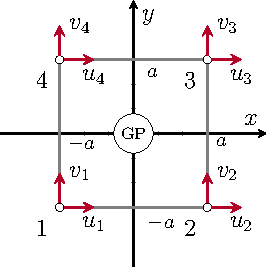
\includegraphics{figures/03_comparison_TO_TTO/03_gauss_point/gp.pdf}
    \caption{A four-node quadrilateral element. GP is the Gaussian integration point for which the equivalent stress is evaluated.}
    \label{fig:03_gp}
\end{marginfigure}


The stress tensor is evaluated using the elasticity Hooke's law in 2D as follows: 
\begin{equation}
    \begin{pmatrix}
    \sigma_x \\
    \sigma_y \\
    \tau_{xy}
    \end{pmatrix}
    =\matr{C}_e
    \begin{pmatrix}
    \varepsilon_\text{x} \\
    \varepsilon_\text{y} \\
    \gamma_{xy}
%     \end{pmatrix},
%     \quad
%    \text{with }
    \end{pmatrix}
    \quad
    \text{with}
    \quad
    \matr{C}_e = \frac{E}{1-\nu^2}
    \begin{pmatrix}
    1   &   \nu &   0   \\
    \nu &   1   &   0   \\
    0   &   0   &   G
    \end{pmatrix}.
\end{equation}

The equivalent Von Mises stress of the element can then be written as:
\begin{align}
    \langle \vect{\sigma}_{\text{VM}} \rangle &= \sqrt{\sigma_x^2 + \sigma_y^2 - \sigma_x \sigma_y+3\tau_{xy}} \\
    &= \sqrt{
    \begin{pmatrix}
    \sigma_x & \sigma_y & \tau_{xy}
    \end{pmatrix}
    \begin{pmatrix}
    1       &   -1/2    &   0   \\
    -1/2    &   1       &   0   \\
    0       &   0       &   3
    \end{pmatrix}
    \begin{pmatrix}
    \sigma_x \\
    \sigma_y \\
    \tau_{xy}
    \end{pmatrix}} \\
    &= \sqrt{\vect{q}_s^T\matr{B}_s^T\matr{C}_e^T\matr{D}_{\text{VM}}\matr{C}_e\matr{B}_s\vect{q}_s}
    \textrm{,  with } \matr{D}_{\text{VM}} = 
    \begin{pmatrix}
    1       &   -1/2    &   0   \\
    -1/2    &   1       &   0   \\
    0       &   0       &   3
    \end{pmatrix} \\
    \langle \vect{\sigma}_{\text{VM}} \rangle &= \sqrt{\vect{q}_s^T\matr{S}\vect{q}_s}, \quad
    \textrm{with } \matr{S} = \matr{B}_s^T\matr{C}_e^T\matr{D}_{\text{VM}}\matr{C}_e\matr{B}_s.
    \label{eq:03_VM_calc}
\end{align}
\paragraph{Microscopic and macroscopic stress}
In stress-constrained topology optimization, the element stress is usually evaluated using the microscopic stress formulation, assuming that there is no direct correlation between stress and density~\sidecite{duysinx_topology_1998}. Indeed, the use of the macroscopic stress in volume minimization optimization problems creates an all-void design~\sidecite{le_stress-based_2010}. The properties that the microscopic stress should present are:
\begin{enumerate}[label=(\roman*)]
    \item The stress criterion should be mathematically as simple as possible, as the relationship between Young's modulus and density. This permits a simple numerical implementation.
    \item To mimic the real physical behavior, the microscopic stress should be inversely proportional to density.
    \item The microscopic stress should converge to a non-zero value at zero density. This requisite is deduced from investigations into the asymptotic stress behavior in thin layers~\sidecite{verbart_unified_2017}.
\end{enumerate}

The relation between stress and displacement is written as:
\begin{equation}
    \langle \vect{\sigma}_{\text{VM}} \rangle = \matr{C}_e(\langle E \rangle) \langle \vect{\varepsilon} \rangle,
    \label{eq:03_stress_disp}
\end{equation}
where the variables between angular brackets $\langle \dots \rangle$ represent macroscopic variables.

Combining (i) and (ii) with \eqsref{eq:03_simp} and \eqrefnotext{eq:03_stress_disp}, the microscopic stress can be written as:
\begin{equation}
    \vect{\sigma}_{\text{VM}} = \frac{\langle \vect{\sigma}_{\text{VM}} \rangle}{\rho^q_e} = \rho_e^{p-q} \matr{C}_e(E_0)\langle \vect{\varepsilon} \rangle,
\end{equation}
where the exponent $q$ is a number greater than 1.

One possible choice that satisfy all the requirements is $q=p$~\sidecite{le_stress-based_2010,verbart_unified_2017,holmberg_stress_2013,da_silva_stress-constrained_2019}. Thus, the microscopic stress is defined as:
\begin{equation}
    \vect{\sigma}_{\text{VM}} = \matr{C}_e(E_0)\langle \vect{\varepsilon} \rangle.
    \label{eq:03_micro_stress}
\end{equation}
From a physical perspective, the significance of microscopic stress becomes evident when considering an element with intermediate density and a porous microstructure. The microscopic stress presented in \eqref{eq:03_micro_stress} measures the stress of the microstructure. It is grounded in the assumption that the macroscopic deformations of the homogenized element generate within the microstructure of the element a stress state that remains unaffected by the density of the element itself.

\paragraph{Constraints aggregation and relaxation}
When optimizing a structure with stress constraints using a \gls{nand} formulation, two primary challenges commonly arise:
\begin{enumerate}[label=(\roman*)]
    \item Is it known in the literature \cite{rozvany_design-dependent_2001,stolpe_models_2003} that stress-based topology optimization suffers from the \textit{singular minima} (or \textit{singularity}) problem: firstly observed on truss structure optimization \cite{sved_structural_1968}, these \textit{minima} are almost inaccessible to a standard gradient-based optimizer, and they represent the \textit{minima} of the optimization. This is because achieving the optimal solution to a problem using continuous design variables may necessitate passing through a state where the optimization constraints are violated, \ie the \textit{minimum} is on a lower dimension compared to the design space. This problem is often solved using a technique called \textit{constraints relaxation}~\sidecite{cheng_relaxed_1997}.

    \item The stress is a local measure, and thus a large set of constraints is generated when a reasonably fine mesh is used (one element, one constraint). This problem is often solved using a technique called \textit{constraints aggregation} or \textit{global constraints}~\sidecite{da_silva_local_2021}.
\end{enumerate} 

Following the work developed by Verbart \etal~\sideciteonce{verbart_unified_2017}, the lower bound \gls{ks} function~\sidecite{kreisselmeier_systematic_1979} is used to approximate the local relaxed stress constraint maximum. The authors discovered that employing lower-bound \gls{ks} aggregation functions to approximate the maximum operator in stress-constrained topology optimization eliminates the need for stress constraint relaxation methods to address the singularity issue. This is because the lower-bound functions inherently offer a combined effect of constraint aggregation and relaxation. The \gls{ks} aggregated stress constraint function is defined as follows:
\begin{equation} 
    G_{\text{KS}}^\text{L} = \frac{1}{P} \ln{\left( \frac{1}{N_\text{e}} \sum e^{{P}\bar{g}_i} \right)}.
    \label{eq:03_gksl}
\end{equation}
Its main advantage over other different formulations is that it uses a single hyperparameter $P$ to control the aggregation and the relaxation of the constraints simultaneously.

\paragraph{Minimum volume formulation}
The \gls{nand} minimum volume formulation for continuous discretization is written combining \eqsref{eq:03_obj_vol} and \eqrefnotext{eq:03_gksl} as:
\begin{equation}
    \begin{aligned}
    \min_{\bm{\rho}}         && V &= \frac{1}{N_{e}} \sum_{i \in \Omega} \rhophys_i,  \\
    \textrm{s.t.}   && G_{\text{KS}}^\text{L} &= \frac{1}{P} \ln{\left( \frac{1}{N_\text{e}} \sum_{i \in \Omega} e^{{P}\bar{g}_i} \right)} \leq 0 \\
    && \bm{K}\bm{u} &= \bm{F}\\
    && 0 &\leq \rho_i \leq 1, \\
    \end{aligned}
    \tag{$\mathbb{T}_1$}
    \label{eq:03_prob-stress}
\end{equation}
The optimization is carried out using a gradient descent optimization algorithm for which the sensitivities are given in analytical form. Using analytic gradients is in general more efficient than finite differences as it avoids the need for multiple function evaluations, making the optimization process faster and more precise.

\paragraph{Sensitivity analysis of the objective function}
The objective of this section is to quickly present the calculation of the analytical sensitivity of the volume with respect to the design variable $\rho$. Deriving \eqref{eq:03_obj_vol} we obtain:

\begin{equation}
    \derfrac{V}{\rhophys_i} = \frac{1}{N_{e}}.
    \label{eq:03_01}
\end{equation}
The sensitivity of the objective function can then be evaluated using \eqsref{eq:03_01} \eqrefnotext{eq:03_sens_filt}, \eqrefnotext{eq:03_sens_proj}, and \eqrefnotext{eq:03_chain} as follows:
\begin{equation}
    \frac{d V}{d \rho_i} = \sum_{j \in \mathbb{N}_{i,R}} \derfrac{V}{\rhophys_j} \derfrac{\rhophys_j}{\rhofil_j} \derfrac{\rhofil_j}{\rho_i}.
\end{equation}
\paragraph{Sensitivity analysis of the constraint function}
This section focuses on the details of the calculation of how the constraint function $G_{\text{KS}}^\text{L}$ changes with respect to the design variable $\vect{\rho}$.

As the constraint function $G_{\text{KS}}^\text{L} = G(\vect{\rhophys}, \vect{u}(\vect{\rhophys}) )$ is explicitly and implicitly (via the relationship with $\vect{u}$) depending on $\vect{\rhophys}$, the first-order derivative is evaluated using the total derivative formula:
\begin{equation} \label{eq:03_sens-0}
    \derfrac{G_{\text{KS}}^\text{L}}{\rhophys_j} = \frac{d G}{d \rhophys_j} = \derfrac{G}{ \rhophys_j} + \derfrac{G}{\vect{u}} \frac{d \vect{u} }{d \rhophys_j}.
\end{equation}
As function $G_{\text{KS}}^\text{L}$ depends on $\vect{u}$ via the stresses $\sigma_i$, it is possible to write:
\begin{equation} \label{eq:03_sens-1}
    \derfrac{G}{\vect{u}} = \sum_{i \in \Omega} \left( \derfrac{G}{\sigma_i} \derfrac{\sigma_i}{\vect{u}}\right).
\end{equation}
Combining Eq. \ref{eq:03_sens-0} with Eq. \ref{eq:03_sens-1}, we obtain:
\begin{equation} \label{eq:03_sens-2}
    \frac{d G}{d \rhophys_j} = \underbrace{\derfrac{G}{\rhophys_j}}_A + \sum_{i \in \Omega} \left( \underbrace{\derfrac{G}{\sigma_i}}_B \underbrace{\derfrac{\sigma_i}{\vect{u}}}_C \right)  \underbrace{\frac{d \vect{u} }{d \rhophys_j}}_D.
\end{equation}
We compute the four factors separately:
\begin{enumerate}[label=\Alph* --]
    \item The first term represents the explicit relationship of $G$ to the physical densities and its calculation is straightforward: 
    \begin{equation} \label{eq:03_sens-2-1}
        \derfrac{G}{ \rhophys_j} = \frac{1}{P} \frac{\left(\frac{ \sigma_{\text{VM},j}}{\sigma_L}-1 \right)\frac{1}{N_\text{e}} P e^{{P}\bar{g}_j}}{\frac{1}{N_\text{e}} \sum_k e^{{P}\bar{g}_k}} = \left(\frac{ \sigma_{\text{VM},j}}{\sigma_L}-1 \right) \frac{e^{{P}\bar{g}_j}}{\sum_k e^{{P}\bar{g}_k}}.
    \end{equation}
    
    \item The second term can be calculated using the chain rule:
    \begin{equation}
        \label{eq:03_sens-2-2}
        \derfrac{G}{\sigma_i} = \derfrac{G}{\bar{g}_i} \derfrac{\bar{g}_i}{\sigma_i} = \frac{1}{P} \frac{\frac{1}{N_\text{e}} P e^{{P}\bar{g}_i}}{\frac{1}{N_\text{e}} \sum_k e^{{P}\bar{g}_k}} \frac{\rhophys_i}{\sigma_L} = \frac{\rhophys_i}{\sigma_L} \frac{e^{{P}\bar{g}_i}}{\sum_k e^{{P}\bar{g}_k}}.
    \end{equation}
    
    \item We reformulate \eqref{eq:03_VM_calc} to be written in global coordinates instead of local:
    \begin{equation}
        \label{eq:03_sens-3}
        \sigma_i^2 = \vect{q}_s^T\matr{S}\vect{q}_s = \vect{u}^T |\matr{S_i}|_g \vect{u},
    \end{equation}  
    where $|\matr{S_i}|_g$ represents the matrix $\matr{S}$ of \eqref{eq:03_VM_calc}written on global coordinates \sidenote{The matrix $|\matr{S_i}|_g$ can be calculated using the very same assembling approach used for the stiffness matrix $\matr{K}$ starting from the elemental stiffness matrix $\matr{K}_e$. As the global stiffness matrix $\matr{K}$, $|\matr{S_i}|_g$ is symmetric and sparse.}. We can now differentiate \eqref{eq:03_sens-3} with respect of the displacement field in global coordinates $\vect{u}$ to obtain:
    \begin{equation}
        \label{eq:03_sens-4}
        \derfrac{\sigma_i}{\vect{u}} = \frac{|\matr{S_i}|_g \vect{u}}{\sigma_i}.
    \end{equation}
    \eqsref{eq:03_sens-2-2} and \eqrefnotext{eq:03_sens-4} are now combined to obtain the result of the product of the \textbf{B} and \textbf{C} terms. As a result, the derivatives of $G$ with respect to $\bm{u}$, are written as:
    \begin{equation} \label{eq:03_sens-4-1}
        \derfrac{G}{\vect{u}} = \frac{\frac{\rhophys_j}{\sigma_L\sigma_j} e^{{P}\bar{g}_i}}{\sum_i e^{{P}\bar{g}_i}} |\bm{S_j}|_g \bm{u}.
    \end{equation}

    \item To calculate the last term, we take the static equilibrium equation $\matr{K}\vect{u} = \vect{f}$ and differentiate it with respect to the physical densities $\rhophys_j$, obtaining:
    \begin{equation}
        \derfrac{\matr{K}}{\rhophys_j}\vect{u} + \matr{K}\derfrac{\vect{u}}{\rhophys_j} = 0 \iff \derfrac{\vect{u}}{\rhophys_j} = -\matr{K}^{-1}\derfrac{\matr{K}}{\rhophys_j}\vect{u},
    \end{equation}
    where
    \begin{equation}
        \label{eq:03_sens-5}
        \derfrac{\matr{K}}{\rhophys_{j}} = (E_0-E_{\textrm{min}}) p\rhophys_j^{p-1} \matr{K}_{e,j}.
    \end{equation}
    \eqref{eq:03_sens-5} represent the well-known first-derivative term of the global stiffness matrix $\matr{K}$ with respect to the physical densities $\rhophys_j$ when using \gls{simp} material scheme~\sidecite{bendsoe_topology_2004}. We finally obtain the last term:
    \begin{equation} \label{eq:03_sens-6}
        \frac{d \vect{u} }{d \rhophys_j} = - \matr{K}^{-1} \left((E_0-E_{\textrm{min}}) p\rhophys_j^{p-1} \matr{K}_e \right) \vect{u}.
    \end{equation}
\end{enumerate}

Combining Eq. \ref{eq:03_sens-2}, Eq. \ref{eq:03_sens-2-1}, Eq. \ref{eq:03_sens-4-1}, and Eq. \ref{eq:03_sens-6}, we finally obtain:
\begin{equation}
\derfrac{G_{\text{KS}}^\text{L}}{\rhophys_j} = \left(\frac{ \sigma_{\text{VM},j}}{\sigma_L}-1 \right) \frac{e^{{P}\bar{g}_j}}{\sum_k e^{{P}\bar{g}_k}} - 
\matr{K}^{-1}\derfrac{G}{\vect{u}} \left(\derfrac{\matr{K}}{\rhophys_{j}} \right) \vect{u}.
\end{equation}

To avoid the explicit calculation of $\matr{K}^{-1}$ we use the \textit{adjoint method}\sidenote{More information about the adjoint method used to analytically calculate the first-order derivatives can be found on the Martins \etal book \cite{martins_engineering_2021}.}. Here is the linear system that, once solved, permits to calculate $\vect{\psi}$:
\begin{equation} \label{eq:03_sens-98}
    \matr{K}\vect{\psi} = \derfrac{G}{\vect{u}} \iff \vect{\psi} = \matr{K}^{-1}\derfrac{G}{\vect{u}}.
\end{equation}
This formula is called \textit{adjoint equation}. This equation is solved for $\vect{\psi}$ and the result used to evaluate:
\begin{equation}\label{eq:03_sens-99}
\derfrac{G_{\text{KS}}^\text{L}}{\rhophys_j} = \left(\frac{ \sigma_{\text{VM},j}}{\sigma_L}-1 \right) \frac{e^{{P}\bar{g}_j}}{\sum_k e^{{P}\bar{g}_k}} - \vect{\psi} \left(\derfrac{\matr{K}}{\rhophys_{j}}\right) \vect{u}.
\end{equation}
\marginnote{Solving linear system \ref{eq:03_sens-98} instead of directly calculating the inverse matrix of $\matr{K}$ is more efficient from a performance perspective. The cost of solving a system using the Cholesky decomposition is $\mathcal{O}(N^3/3)$, while a matrix inversion is $\mathcal{O}(N^3)$.} where $N$ represents the size of the square matrix describing the linear system.
\eqref{eq:03_sens-99} represents the first-order derivative equation used to evaluate the sensitivity of the constraint function $G_{\text{KS}}^\text{L}$ with respect to the physical densities $\vect{\rhophys}$. The value of $\vect{\psi}$ is calculated every iteration solving the linear system \ref{eq:03_sens-98}.

The sensitivity of the aggregated constraint function with respect to the design variable $\vect{\rho}$ is evaluated using \eqsref{eq:03_01} \eqrefnotext{eq:03_sens_filt}, \eqrefnotext{eq:03_sens_proj}, and \eqrefnotext{eq:03_chain} as follows:
\begin{equation} \label{eq:03_chain_sens_fin}
    \frac{d G_{\text{KS}}^\text{L}}{d \rho_i} = \sum_{j \in \mathbb{N}_{i,R}} \derfrac{G_{\text{KS}}^\text{L}}{\rhophys_j} \derfrac{\rhophys_j}{\rhofil_j} \derfrac{\rhofil_j}{\rho_i}.
\end{equation}

\subsection{Truss discretization \gls{sand} minimum volume formulation}
We are now shifting our focus from continuous structures to discrete truss systems, describing the \acrfull{tto} (also known in early literature as layout optimization), a structure optimization method that focuses on discrete structures. In his most used formulation, \gls{tto} aims at reducing material usage while meeting stress criteria using a \gls{sand} approach. The problem is already well-posed for comparison with continuous discretization, and we intend to explore specific key concepts within its established framework.
\paragraph{Classical Michell structures} \label{sec:03_michell}
The characteristics of these structures are described by some simple criteria that date to the end of the 19th and the beginning of the 20th century. When a structure is statically determinate — \ie the structure is not a mechanism, and it is not over-constrained by the supports — the Maxwell theorem~\sidecite{maxwell_ireciprocal_1870} states that:
\begin{equation} \label{eq:03_maxwell-th}
    \sum_{\forall i | q_i>0}\ell_iq_i + \sum_{\forall i | q_i<0}\ell_iq_i = \textrm{const.}
\end{equation}
where $\ell_i$ and $q_i$ represent the length and the axial force of the $i$-th member, respectively. The constant value at the right of~\eqref{eq:03_maxwell-th} depends on the nature of the boundary conditions and the material used. The Maxwell theorem dictates that any increment in compression forces must be counterbalanced by an equivalent increase in tension forces when the structure remains topologically unchanged. So for statically determinate structures the structure layout is not influenced by the ratio between $\sigma_\text{c}$ and $\sigma_\text{t}$, Young's modulus $E$ of the material, nor the force magnitude.

Starting from Maxwell's findings, Michell theorized two further criteria for optimal truss structures~\sidecite{michell_limits_1904} valid when the maximum allowable stress is equal in tension and compression ($\sigma_\text{t} = \sigma_\text{c}$) and when the supports of the structure are statically determinate. The first one states that all the members of an optimal structure should present internal stress equal in magnitude to the maximum allowable value of the material -- \ie the structure is \textit{fully stressed}. The second criterion asserts that the strain of all the members of the structure should be equal and there should be no other point having a strain higher than this value. As formulated, these two criteria are known as the Michell criteria. The second criterion was later generalized by Hemp~\sidecite{hemp_optimum_1973} as:
\begin{equation} \label{eq:03_hemp}
    -\frac{1}{\sigma_\text{c}}\leq \varepsilon \leq \frac{1}{\sigma_\text{t}}.
\end{equation}
Compared to the second Michell criterion, \eqref{eq:03_hemp} permits to correct identification of the minimum volume structure even when different strength values for compression and tension and different support types are taken. These criteria are known as the Michell-Hemp criteria.

\paragraph{Plastic material formulation}
The rigid-plastic formulation characterizes the material as entirely rigid up to the point of reaching the yield stress, denoted as $\sigma_y$, and subsequently assumes a constant stress level of $\sigma_y$ once that threshold is exceeded. This formulation is a clear consequence of the application of the Michell-Hemp criteria and has thus been used in the very first work of layout optimization (also known as \gls{tto})~\sidecite{dorn_automatic_1964,chan_optimum_1964,hemp_optimum_1973}. 

\paragraph{The ground structure approach}
The ground structure is a framework composed of various structural members that connect specified points or nodes in two- or three-dimensional space (see \figref{fig:03_mesh_d}). These members can take the form of beams, columns, wires, or bars elements, depending on the specific structural requirements. In this thesis, we will deal with trusses, and so the chosen element is the bar. Since the nodes within the ground structure are considered pin-joints, all straight members exclusively face either tension or compression loads. 
\begin{marginfigure}
    \centering
    \includegraphics{figures/03_comparison_TO_TTO/04_disc_mesh/d_mesh.pdf}
    \caption{The domain $\Omega$ is discretized using a set of straight members connecting a set of nodes. This framework is known as the ground structure.}
    \label{fig:03_mesh_d}
\end{marginfigure}

Depending on how the connectivity of the grid of nodes is, we can experience very different ground structures. In a fully connected ground structure, every node within the system is linked to every other node, resulting in a dense and redundant structural configuration. The number of bars $N_{\text{el}}$ of a fully connected ground structure can be determined using the following formula:
\begin{equation}
    N_{\text{el}} = \frac{M \cdot (M-1)}{2},
\end{equation}
where $M$ represents the number of nodes of the structure.

In classic works, the ground structure is used as the start of the optimization, where the optimized structure is obtained as a subset of the initial ground structure, but multiple alternative approaches have been proposed since then, \eg starting from a very coarse ground structure that is enriched during the analysis~\sidecite{gilbert_layout_2003}, or giving the nodes of a coarse ground structure the possibility to move, during~\sidecite{pedersen_optimal_1973, achtziger_simultaneous_2007, descamps_lower-bound_2013}, or after the optimization, simultaneously reducing the number of active members of the solution~\sidecite{he_rationalization_2015, lu_reducing_2023}.

\paragraph{Optimization formulation}
The volume minimization formulation with maximum stress constraints is stated in terms of members' cross-sectional areas $\vect{a}$ and member forces $\vect{q}$ as follows:
\begin{equation}
    \begin{aligned}
    \min_{\vect{a}, \vect{q}}   && V &= \vect{\ell}^{T}\vect{a} && \textrm{(Volume minimization)}\\
    \textrm{s.t.}   && \matr{B}_s\vect{q} &= \vect{f} && (g_\text{eq})\\
    && -\sigma_\text{c}\vect{a} &\leq \vect{q} \leq \sigma_\text{t}\vect{a} && (g_\text{st,c}, \; g_\text{st,t}) \\
    && \vect{a} &\geq 0, \\
    \end{aligned}
    \tag{$\mathbb{P}_0$}
    \label{eq:03_optim_original}
\end{equation}
where $\matr{B}_s$ is a $N_{\text{dof}} \times N_{\text{el}}$ matrix containing the direction cosines of the $j$-th member with respect to the $i$-th degree of freedom to calculate the nodal force equilibrium constraints $\vect{g}_\text{eq}$, and where $N_{\text{dof}}$ is the number of \gls{dofs}, equal to $2M$ or $3M$ for a two- or a three-dimensional load case, respectively. $\vect{q} = [q_1, q_2, \ldots,q_{N_{\text{el}}}]^T$ is the vector containing the internal member forces, with a positive sign when in tension, caused by the external load $\vect{f} = [f_1, f_2, \ldots,f_{N_{\text{dof}}}]^T$. The state variable $\vect{a} = [a_1, a_2, \ldots,a_{N_{\text{el}}}]^T$ represents the cross-sectional area of the $N_{\text{el}}$ members of the structure. $\sigma_\text{c}$ and $\sigma_\text{t}$ are the compressive and tensile maximum allowable stresses of the material, respectively, used in the stress constraints $\vect{g}_\text{st,c}$ and $\vect{g}_\text{st,t}$. This formulation takes into account only the linear behavior of the structure and is equivalent to the original and well-studied member force formulation~\sidecite{dorn_automatic_1964, bendsoe_topology_2004}.

The resolution of Problem \ref{eq:03_optim_original} frequently produces complex structures made up of a multitude of small members that tend to the shapes of Michell structures (see Fig~\ref{fig:03_truss-ex})~\sidecite{michell_limits_1904,gilbert_layout_2003}. While it is known that these structures are nearly optimal, one would want to limit the complexity of the resulting structure. Substituting $\vect{\ell}$ with $\vect{\tilde{\ell}} = [\ell_1 + s, \ell_2 + s, \ldots,\ell_{N\text{el}} + s]^T$ in the objective function of \ref{eq:03_optim_original}, one would penalize the appearance of small members~\sidecite{parkes_joints_1975}. $\vect{\tilde{\ell}}$ is called augmented member length and $s$ the joint cost. This approach mimics the mesh-independency regularization filter of topology optimization, avoiding the inevitable apparition of structures with tiny features when a fine mesh is adopted.

\begin{marginfigure}
    \centering
    \includegraphics[width=\linewidth]{figures/03_comparison_TO_TTO/truss-ex.png}
    \caption{The optimal structures found by layout optimization tend at Michell-like structures, made up of a very large number of infinitesimal struts \cite{gilbert_layout_2003}.}
    \label{fig:03_truss-ex}
\end{marginfigure}

\section{Comparison between continuous and truss discretization} \label{sec:03_comparison}
In the upcoming discussion, we will be comparing the optimized structures using discrete and continuous meshes. Our primary objective in this comparison is to gain a comprehensive understanding of the application limits inherent in these two structural discretization methods. If, indeed, we identify such limitations, the aim is to discern and define them. Such discussions have already been pointed out in the literature~\sidecite{bendsoe_optimal_1989, watts_simple_2019}, but they are usually only empirical considerations and not numerical analysis.

Since our interest is in ultralight structures, we are especially interested in comparing the results of both optimization methods when dealing with different volume fractions on a common load case. Since we can't directly control volume in our formulation, we will adjust the material properties to influence the volume fraction of the optimized structure. For this comparative analysis, we have selected three key performance metrics: the volume fraction $V_\text{f}=V/\Omega$, the structural compliance $C$, and the maximum material allowable $\sigma_L$. Among these, we classify stress limit as the active metric used to influence the optimization, while volume and compliance are the objective of the optimization and a passive metric, respectively. In addition to the aforementioned performance metrics, we will also track the execution time of the algorithms.

\subsection{Definition of a common test case}
\begin{figure}
    \centering
    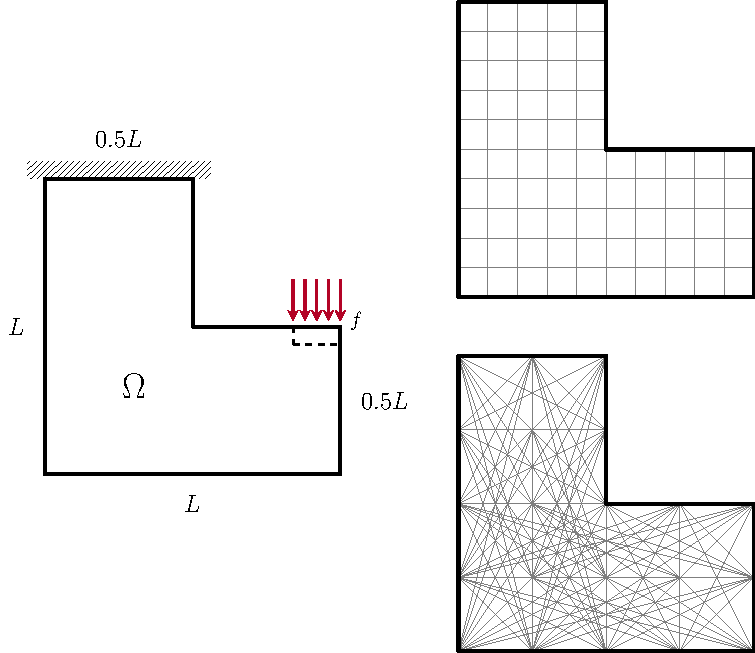
\includegraphics[scale=0.75]{figures/03_comparison_TO_TTO/06_L_bc/L_bc.pdf}
    \caption{On the left, plot of the L-shape beam test case, on the right the graphical representations of the two discretizations used, the continuous (above) and the truss-like (below).}
    \label{fig:03_L_bc}
\end{figure}
The L-shape beam is one of the most used load case benchmarks for stress-based topology optimization~\sidecite{duysinx_topology_1998,le_stress-based_2010}. This choice is driven by the distinctive geometry of the problem, which generates a stress concentration, particularly at the sharp corner—a phenomenon approaching infinity. Consequently, optimized solutions often feature a large fillet, mitigating the intensity of the stress singularity. The geometric description of the test case is given in \figref{fig:03_L_bc}. The beam with dimensions $L\times L$ presents an encastre on the top part and a load on the right extremity. For the continuous mesh case the load is distributed over multiple elements (5\% of $L$) to avoid stress concentrations and the stress constraints are not evaluated there. This zone is considered outside of the design domain $\Omega$.

To permit the discretization comparison, the structure is divided into two distinct meshes: in the continuous case, we employ a mesh consisting of $600\times600$ quadrilateral elements, totaling \num[group-separator={$\,$}]{270000} elements, while for the truss configuration, we employ a mesh with $33\times 33$ nodes and a fully connected ground structure, comprising a total of \num[group-separator={$\,$}]{305728} candidates.

We employ the same isotropic material and structure dimensions for the two optimizations, and the complete data is resumed in \tabref{tab:03_mat}. The value of the maximum material admissible $\sigma_\text{L}$ is used as the parameter that influences the volume fraction of the solutions. For simplicity, all numeric values are assumed normalized and dimensionless.

\begin{margintable}
    \small
    \centering
    \begin{tabular}{cc}
    \toprule
    \textbf{Parameter}        & \textbf{Value} \\ \midrule
    $E$              & 1     \\
    $\nu$            & 0.3   \\
    $L$              & 100   \\
    $\sigma_\text{L}$ & var. \\
    \bottomrule
    \end{tabular}
    \caption{Material data used for the optimizations. The value of the maximum material admissible $\sigma_\text{L}$ is used as the parameter to generate multiple optimized topologies.}
    \label{tab:03_mat}
\end{margintable}

\subsection{Numerical application} \label{sec:03_applications}
The focus of this section is to provide the numerical framework used to carry out the comparative analysis of the optimization results obtained from continuous and truss discretizations. The optimization formulations previously described have been implemented using Python.

The optimizing algorithm chosen for the continuous mesh is the \gls{mma}~\sidecite{svanberg_method_1987}. The parameter called \textit{movelimit}\sidenote{More information on the implementation of the \textit{movelimit} parameter can be found on the paper by Verbart \cite{verbart_unified_2017}} is set to $0.1$ while the other algorithm's parameters are set to their default value. A continuation scheme for the aggressiveness of the projection parameter $\beta$ is set to increase by one every 200 iterations, the number of max iteration is set to 7500, the stopping criteria is calculated as $\Vert r_k \Vert_2 / \sqrt{N_\text{e}}$ on the physical densities $\rhophys$ \cite{ferrari_new_2020}, and it is set to $10^{-4}$. The aggregation parameter $P$ of the aggregation function $G_{\text{KS}}^\text{L}$ is set to 32. The numerical implementation is carried out using the NLopt Python optimization framework~\sidecite{NLopt_2007}, analytically evaluating the sensitivity using \eqsref{eq:03_01} and \eqrefnotext{eq:03_sens-2}.

Formulation \ref{eq:03_optim_original} represents a \gls{lp} problem that can be efficiently solved by modern algorithms. In this work, we used the Python package CVXPY 1.2.2~\sidecite{diamond_cvxpy_2016} with the ECOS 2.0.7~\sidecite{domahidi_ecos_2013} solver. The joint cost $s$ is set to 0.001 and the stopping criteria is chosen as $\norm{\Delta \vect{x}}_\infty \leq 10^{-8}$. As Formulation is linear, no sensitivity calculation is carried out.

The optimizations presented in this section are performed on a server equipped with an Intel® Xeon® CPU E5-2650 @ \qty{2.20}{GHz} and using \qty{8}{GB} of RAM.

\paragraph{Coninuous mesh optimization results}
\begin{figure*}
    \subcaptionbox{}{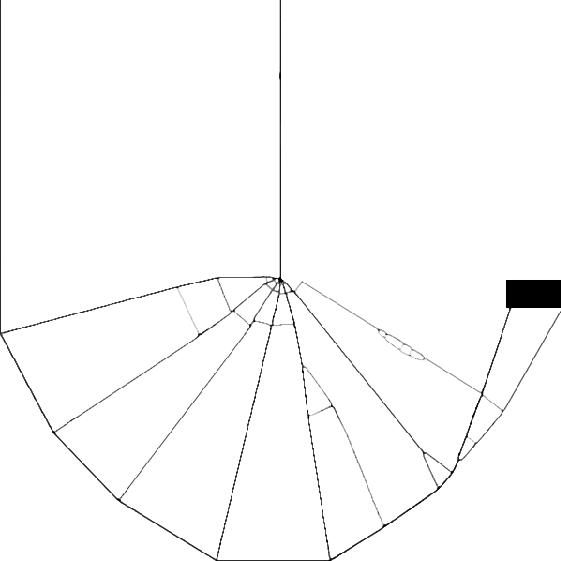
\includegraphics[width=0.23\linewidth ]{figures/03_comparison_TO_TTO/07_to_sol/fig0_10.pdf}}
    \hfill
    \subcaptionbox{}{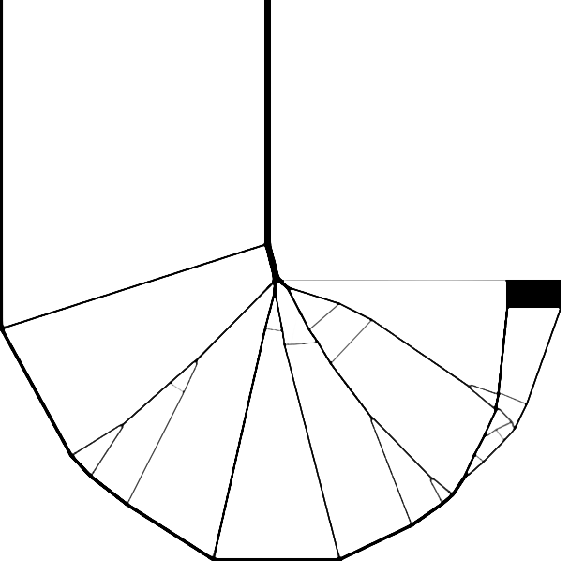
\includegraphics[width=0.23\linewidth ]{figures/03_comparison_TO_TTO/07_to_sol/fig0_2.pdf}}
    \hfill
    \subcaptionbox{}{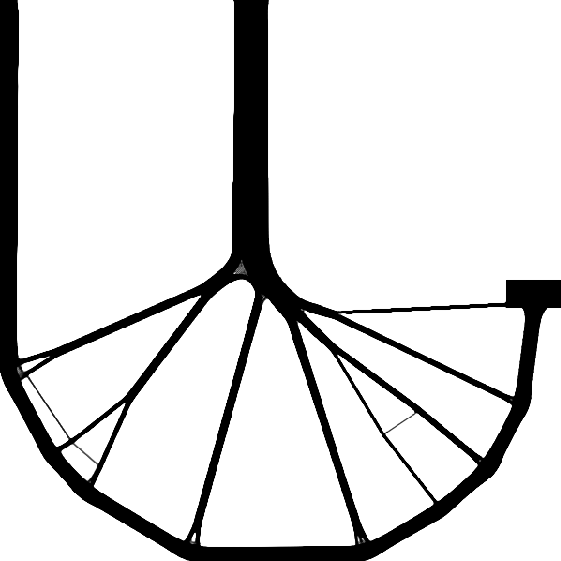
\includegraphics[width=0.23\linewidth ]{figures/03_comparison_TO_TTO/07_to_sol/fig0_0.4.pdf}}
    \hfill
    \subcaptionbox{}{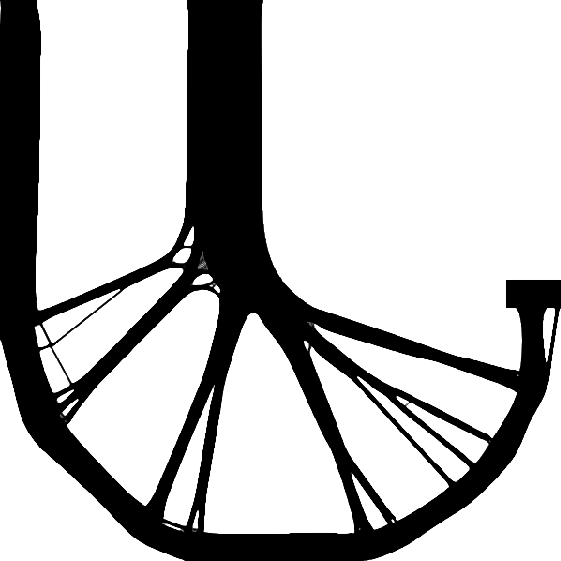
\includegraphics[width=0.23\linewidth ]{figures/03_comparison_TO_TTO/07_to_sol/fig0_0.25.pdf}}
    \bigskip
    \subcaptionbox{}{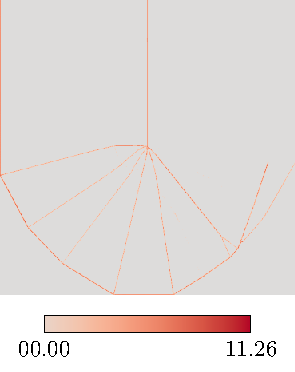
\includegraphics[width=0.23\linewidth ]{figures/03_comparison_TO_TTO/07_to_sol/stress_10.pdf}}
    \hfill
    \subcaptionbox{}{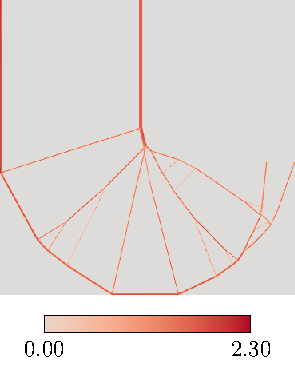
\includegraphics[width=0.23\linewidth ]{figures/03_comparison_TO_TTO/07_to_sol/stress_2.pdf}}
    \hfill
    \subcaptionbox{}{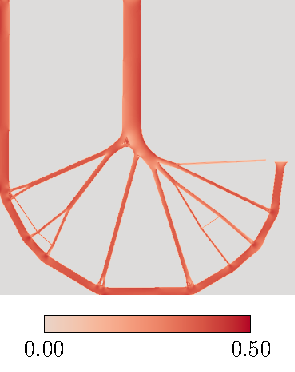
\includegraphics[width=0.23\linewidth ]{figures/03_comparison_TO_TTO/07_to_sol/stress_04.pdf}}
    \hfill
    \subcaptionbox{}{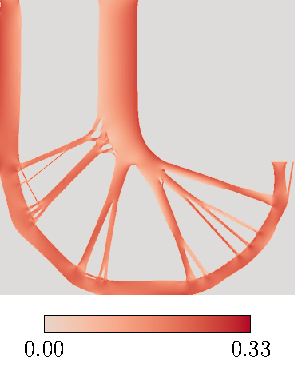
\includegraphics[width=0.23\linewidth ]{figures/03_comparison_TO_TTO/07_to_sol/stress_025.pdf}}
    \caption{(a-d) topology optimized structures for different material admissibles $\sigma_\text{L}=10.00,2.00,0.40\text{ and }0.25$, showing a volume fraction of $V_\text{f}=1.60\%,4.04\%,18.03\%\text{ and }34.71\%$, respectively. (e-h) Von Mises stress distribution of the optimized structures.}
    \label{fig:03_to_sol}
\end{figure*}
In this section, we generate multiple optimized structures with different volume fractions $V_\text{f}$ by launching the optimization code for continuous mesh with different values of the material admissible $\sigma_\text{L}$ spanning from $0.2$ to $20$.

On top of volume fraction, compliance, and stress, we evaluate an additional metric specific to continuous meshes called the \textit{measure of non-discreteness}~\sidecite{sigmund_morphology-based_2007} to evaluate the quality of the solutions. It is defined as:
\begin{equation}
    M_\text{nd} = \frac{\sum_e 4 \rhophys_e(1-\rhophys_e)}{n} \times 100 \%,
\end{equation}
where results near zero mean a completely black-and-white design. 

The results obtained for $\sigma_\text{L}=10.00,2.00,0.40\text{ and }0.25$ are shown in \figref{fig:03_to_sol}. In the upper part of the figure (a-d), we see the topology of the optimized structures with an ascending volume fraction $V_\text{f}$. Interestingly, the topology of the solution remains almost unchanged, varying principally in the thickness of its members. We notice the classic large fillet around the corner that alleviates the stress concentration problem. As the volume decreases, the optimized structure tends to a solution that resembles Michell structures, with a reducing fillet radius. In those cases, we know that the topology optimization algorithm acts as a method for the layout of truss-like structures~\sidecite{bendsoe_generating_1988}. This effect is caused by the combination of different factors, such as the regularization filter, the mesh size, and the low volume fraction~\sidecite{sigmund_non-optimality_2016}. A summary of the numerical results is presented in \tabref{tab:TO_results}.

In the lower part of \figref{fig:03_to_sol} (e-f), we plot the equivalent Von Mises stress for every element of the solution with physical density $\rhophys>0.5$. Multiple interesting observations can be made. First, we notice that the stress distribution is almost uniform in the structure, and it tends to the value of the material admissible $\sigma_\text{L}$ -- \ie we approach a \textit{fully stressed} structure. Even if the geometric support of the theory is different, it looks like the topology-optimized structures follow the Michell criteria presented in \secref{sec:03_michell} for optimal truss structures. Furthermore, it is observed that the maximum stress exceeds the material admissible $\sigma_\text{L}$. Aggregation methods aim to estimate the maximum value of the stress constraint across a group of elements. However, these aggregation methods do not perfectly align with the exact maximum value, which is a recognized limitation. To address this challenge, multiple approaches have been proposed within the aggregation framework to accurately account for the true constraint value, like using a set of active stress constraints~\sidecite{bruggi_topology_2012}, several aggregation clusters~\sidecite{paris_block_2010} or rectifier functions~\sidecite{norato_maximum-rectifier-function_2022}.

Looking again at \tabref{tab:TO_results}, we notice that the optimization processes exhibit long execution times, especially when dealing with extreme cases like high-volume fractions. This effect is likely caused by the very fine mesh used to discretize the design domain $\Omega$, by the sensitivity calculation by means of the adjoint method, and by the increasing difficulty of satisfying the stress constraints.

\begin{table}
    \small
    \centering
    \sisetup{table-auto-round}
    \begin{tabular}{S[table-format = 2.2]
                    S[table-format = 2.2]
                    S[table-format = 2.2]
                    S[table-format = 5.0]
                    S[table-format = 1.2]
                    S[table-format = 4.0]
                    c
                    }
    \toprule
    $\bm \sigma_L$ & $\bm \max \bm \sigma_L$   & $\bm V_\text{f}$     & $\bm C$ & $M_\text{nd}$  & {\textbf{It.}}  & {\textbf{Time}}      \\ \midrule
    20    & 23.51 & 1.18\ppercent       & 6992.10    & \qty{1.91}{\percent} & 1142     & $\hms{08;11;00}$ \\
    10    & 11.26 & 1.60\ppercent       & 3837.08    & \qty{2.19}{\percent} & 1147     & $\hms{07;55;00}$ \\
    8     & 8.78  & 1.74\ppercent       & 2765.60    & \qty{1.95}{\percent} & 792      & $\hms{05;39;00}$ \\
    6     & 7.15  & 1.89\ppercent       & 2243.31    & \qty{1.81}{\percent} & 806      & $\hms{05;35;00}$ \\
    5     & 5.81  & 2.17\ppercent       & 1823.12    & \qty{1.81}{\percent} & 849      & $\hms{05;53;00}$ \\
    4     & 4.69  & 2.67\ppercent       & 1423.54    & \qty{2.02}{\percent} & 894      & $\hms{06;12;00}$ \\
    3     & 3.47  & 3.00\ppercent       & 1132.79    & \qty{1.64}{\percent} & 993      & $\hms{06;45;00}$ \\
    2     & 2.30  & 4.04\ppercent       & 781.48     & \qty{1.45}{\percent} & 1189     & $\hms{08;20;00}$ \\
    1     & 1.18  & 7.28\ppercent       & 403.53     & \qty{1.35}{\percent} & 1621     & $\hms{11;41;00}$ \\
    0.90  & 1.06  & 8.09\ppercent       & 364.80     & \qty{1.31}{\percent} & 1656     & $\hms{11;36;00}$ \\
    0.80  & 0.96  & 8.82\ppercent       & 331.95     & \qty{1.21}{\percent} & 1937     & $\hms{15;21;00}$ \\
    0.70  & 0.84  & 10.05 \ppercent    & 291.89     & \qty{1.09}{\percent} & 1827     & $\hms{13;21;00}$ \\
    0.60  & 0.73  & 11.80 \ppercent    & 250.23     & \qty{1.19}{\percent} & 1955     & $\hms{14;21;00}$ \\
    0.50  & 0.61  & 14.18 \ppercent    & 213.01     & \qty{1.06}{\percent} & 2032     & $\hms{15;39;00}$ \\
    0.40  & 0.50   & 18.03\ppercent     & 169.90     & \qty{1.08}{\percent} & 2259     & $\hms{17;06;00}$ \\
    0.35  & 0.44  & 21.12 \ppercent    & 148.13     & \qty{1.15}{\percent} & 2421     & $\hms{19;29;00}$ \\
    0.30  & 0.38  & 26.21 \ppercent    & 125.69     & \qty{1.50}{\percent} & 3100     & $\hms{24;46;00}$ \\
    0.25  & 0.33  & 34.71 \ppercent    & 104.30     & \qty{1.04}{\percent} & 3484     & $\hms{27;39;00}$ \\
    0.20  & 0.27  & 48.08 \ppercent    & 76.56      & \qty{1.26}{\percent} & \color{accent_r_1}7500     & $\hms{91;46;00}$ \\ \bottomrule
    \end{tabular}
    \caption{Numerical results of the topology optimization method of the L-shape beam load case with varying material admissible $\sigma_\text{L}$ on a $600 \times 600$ elements mesh.}
    \label{tab:03_TO_results}
    \end{table}
    
\begin{marginfigure}
        \centering
        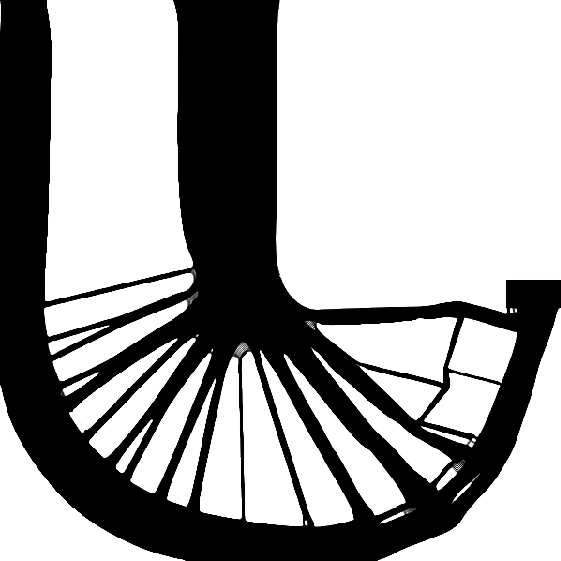
\includegraphics[width=0.8\linewidth]{figures/03_comparison_TO_TTO/08_to_no/fig0.pdf}
        \caption{The optimized structure for $\sigma_\text{L}=0.2$ with $V_\text{f}=\qty{48.08}{\percent}$, but does not converge after 7500 iterations.}
        \label{fig:03_to_sol_no}
    \end{marginfigure}

As previously mentioned, our focus lies in exploring the method's limits, particularly at the volume fraction boundaries. When dealing with excessively weak materials -- \ie materials that show a low $\sigma_\text{L}$, we encounter a scenario where no solution can be attained since no distribution can fulfill the imposed constraints. Throughout our research with this specific test case and mesh size, we did not produce any solutions with a volume fraction exceeding 50\%. Although we haven't reached that scenario with $\sigma_\text{L}$ set to 0.2, the calculation time and the number of iterations increase significantly,showing that we have encountered the method's limits. The calculation time has significantly increased because the algorithm faces greater difficulty in satisfying the stress constraints. \figref{fig:03_to_sol_no} shows the topology of the solution with $\sigma_\text{L}=0.2, \; V_\text{f}=\qty{48.08}{\percent}$ and over five days of optimization.

\begin{marginfigure}
    \centering
    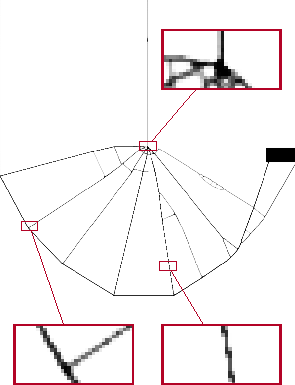
\includegraphics[width=0.8\linewidth]{figures/03_comparison_TO_TTO/09_to_zoom/to_zoom.pdf}
    \caption{The optimized structure for $\sigma_\text{L}=10.0$ with $V_\text{f}=\qty{1.60}{\percent}$. Some of the structure's features present not even a fully-dense element in their thickness.}
    \label{fig:03_to_sol_zoom}
\end{marginfigure}
Conversely, when dealing with exceedingly strong material -- \ie materials that show a high $\sigma_\text{L}$, the optimal scenario would demand such minimal material usage that certain sections of the structure become thinner than the width of a single element. In this case, the mesh used for discretization is too coarse to accurately represent the solution, and finer meshing becomes essential to capture the intricate details of the optimized design. \figref{fig:03_to_sol_zoom} shows
the limit case when $\sigma_\text{L}=10.0$ and $V_\text{f}=\qty{1.60}{\percent}$.

Finally, in \figref{fig:03_to_plot} are the plots summarizing our findings, with the limits highlighted. To effectively show the different orders of magnitude present in the plot, we have used both linear and logarithmic scales simultaneously.
\begin{figure*}
    \hspace*{\fill}
    \subcaptionbox{\label{fig:03_to_plot_lin}}{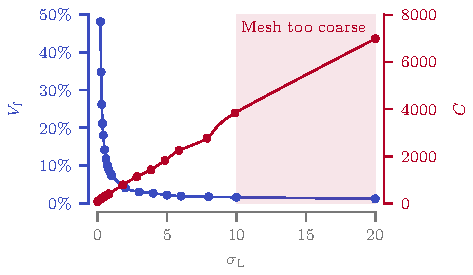
\includegraphics{figures/03_comparison_TO_TTO/10a_to_graph_lin/to_c_lin.pdf}}
    \hfill
    \subcaptionbox{\label{fig:03_to_plot_log}}{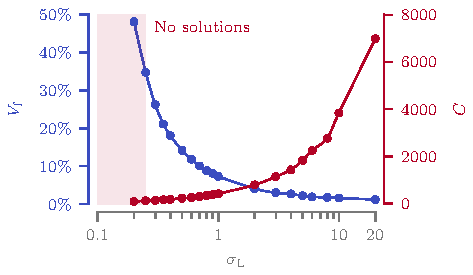
\includegraphics{figures/03_comparison_TO_TTO/10b_to_graph_log/to_c.pdf}}
    \hspace*{\fill}
    \caption{Linear (a) and logarithmic (b) plot of the volume fraction $V_\text{f}$ and the compliance $C$ with respect to the maximum material admissible $\sigma_\text{L}$ for the continuous mesh structures. Areas in red represent the boundaries of the applied method.}
    \label{fig:03_to_plot}
\end{figure*}
It's interesting to note that the volume fraction $V_\text{f}$ follows a hyperbolic relationship, while compliance $C$ exhibits a linear correlation with respect to the material admissible $\sigma_\text{L}$.

\paragraph{Truss mesh optimization results}
In this section, we present the optimized structures of the truss discretization. \figref{fig:03_L_tto} provides a visual representation of the topology and the corresponding stress distribution. Due to the inherent linearity properties of Formulation \ref{eq:03_optim_original}, several intriguing characteristics emerge. Notably, in the case of the tested L-shaped case, we encounter a scenario where the boundary conditions are neither overconstrained nor subject to asymmetric stress constraints. Consequently, this test case aligns with the Michell criteria. As a result, the topology does not vary regardless of the imposed stress limit, and the structure is fully stressed.
\begin{figure}
    \centering
    \hspace*{\fill}
    \subcaptionbox{\label{fig:03_tto_sol_tc}}{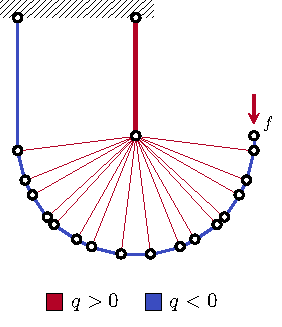
\includegraphics{figures/03_comparison_TO_TTO/11_tto_sol/L_tto_opt.pdf}}
    \hfill
    \subcaptionbox{\label{fig:03_tto_sol_st}}{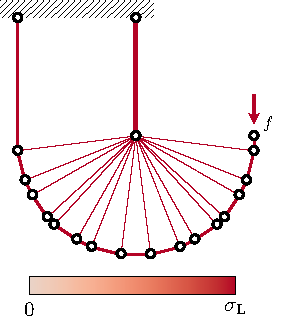
\includegraphics{figures/03_comparison_TO_TTO/11_tto_sol/L_tto_opt_st.pdf}}
    \hspace*{\fill}
    \caption{Topology (a) and stress (b) plot for the truss-like discretization.}
    \label{fig:03_L_tto}
\end{figure}
Additionally, the following equation consistently holds:
\begin{equation} \label{eq:03_V_star}
    V^*=\frac{fL}{\sigma_\text{L}}\cdot \text{const.},
\end{equation}
where the multiplicative constant depends on the load case and the ground structure used to discretize the design space $\Omega$ \sidecite{lewinski_extended_1994}. The execution time of the optimization is approximately \qty{90}{\second} and does not change with respect to the maximum stress $\sigma_\text{L}$. The results of the multiple optimizations can be found in \tabref{tab:03_TTO_results}.

\begin{table}
    \small
    \centering
    \sisetup{table-auto-round}
    \begin{tabular}{S[table-format = 2.1]
                    S[table-format = 2.2]
                    S[table-format = 5.0]
                    S[table-format = 2.1]                    
                    S[table-format = 2.0]}
        
    \toprule
    $\bm \sigma_L$ & $\bm V_\text{f}$     & $\bm C$      & {\textbf{Min} $\bm \lambda$} & {\textbf{Time}} \\ \midrule
    50         & 0.124169\ppercent  & 23281.62 & 111.687                     & $\hms{00;01;06}$    \\
    20         & 0.310422\ppercent  & 9312.65  & 70.637                      & $\hms{00;01;09}$    \\
    10         & 0.620843\ppercent  & 4656.32  & 49.948                      & $\hms{00;01;18}$    \\
    8          & 0.776054\ppercent  & 3725.06  & 44.675                      & $\hms{00;01;15}$    \\
    6          & 1.034739\ppercent  & 2793.79  & 38.689                      & $\hms{00;01;10}$    \\
    5          & 1.241686\ppercent  & 2328.16  & 35.318                      & $\hms{00;01;24}$    \\
    4          & 1.552108\ppercent  & 1862.53  & 31.590                      & $\hms{00;01;18}$    \\
    3          & 2.069477\ppercent  & 1396.90  & 27.358                      & $\hms{00;01;15}$    \\
    2          & 3.104216\ppercent  & 931.26   & 22.337                      & $\hms{00;01;15}$    \\
    1          & 6.208431\ppercent  & 465.63   & 15.795                      & $\hms{00;01;17}$    \\
    0.90       & 6.898257\ppercent  & 419.07   & 14.984                      & $\hms{00;01;20}$    \\
    0.80       & 7.760539\ppercent  & 372.51   & \color{accent_r_1}14.127    & $\hms{00;01;21}$    \\
    0.70       & 8.869187\ppercent  & 325.94   & \color{accent_r_1}13.215    & $\hms{00;01;16}$    \\
    0.60       & 10.347385 & 279.38\ppercent   & \color{accent_r_1}12.235    & $\hms{00;01;20}$    \\
    0.50       & 12.416862 & 232.82\ppercent   & \color{accent_r_1}11.169    & $\hms{00;01;22}$    \\
    \bottomrule    
    \end{tabular}
    \caption{Numerical results of the \gls{tto} method of the L-shape beam load case with varying material admissible $\sigma_\text{L}$ on a $33 \times 33$ ground structure.}
    \label{tab:03_TTO_results}
    \end{table}

    \begin{marginfigure}
        \centering
        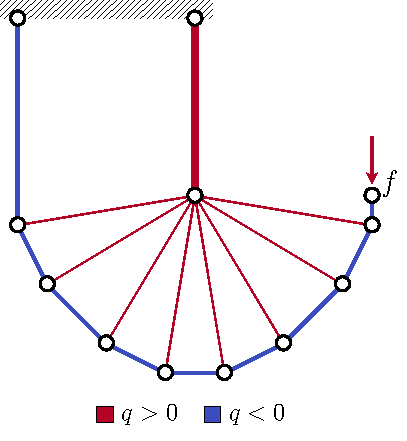
\includegraphics[width=0.8\linewidth]{figures/03_comparison_TO_TTO/12_tto_sol_13/L_tto_opt.pdf}
        \caption{Optimized structure obtained a fully connected ground structure with $13 \times 13$ and \num[group-separator={$\,$}]{7705} candidates.}
        \label{fig:03_L_tto_13}
    \end{marginfigure}
It's worth noting that we have intentionally opted for a fine mesh here to achieve a design variable count roughly equivalent to that of the continuous mesh case. We have utilized a fully connected ground structure with $33 \times 33$ nodes, but in reality, we obtain satisfactory results even with just $13 \times 13$ nodes (see \figref{fig:03_L_tto_13}). In this case we obtain a normalized volume $V^*=4.705 \; fL/\sigma_\text{L}$, signifying a \qty{1.05}{\percent} increase compared to the $33 \times 33$ case with $V^*=4.656 \; fL/\sigma_\text{L}$ with a variable count reduction of \qty{97.4}{\percent} (\num[group-separator={$\,$}]{305728} vs \num[group-separator={$\,$}]{7705} candidates). The computational time remains below one second.

In assessing solution quality, we employ a distinct metric known as the slenderness ratio, denoted as $\lambda$, which represents the ratio between the length and the radius of gyration of the bar. In our specific case, we have established a minimum slenderness ratio of 15. For a bar with a circular cross-sectional area, this corresponds to a radius of $R_\lambda$ for a bar length of $7.5\;R_\lambda$. We higlighted in red the optimized structures that does not repect the minimum slenderness ratio in \tabref{tab:03_TTO_results}. It is important to note that this metric is very sensible to the ground structure used: for example in the $13\times13$ nodes test case, $\lambda$ becomes critical ($\lambda=14.8$) only when $\sigma_\text{L}=0.25$ and $V_\text{f}=25.09$, suggesting that a control of this parameter during the optimization should be beneficial.

Lastly, \figref{fig:03_tto_plot} provides a visual summary of our findings, emphasizing in red the observed limits. To effectively show the different orders of magnitude present in the plot and how already done for the continuous mesh case, we have used both linear and logarithmic scales simultaneously. In this case, the compliance exhibits a perfectly linear relationship, while the volume follows a hyperbolic law in accordance with \eqref{eq:03_V_star}.

\begin{figure*}
    \hspace*{\fill}
    \subcaptionbox{\label{fig:03_tto_plot_lin}}{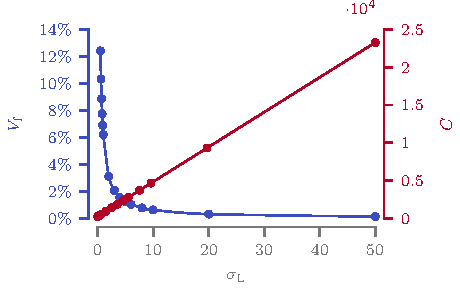
\includegraphics{figures/03_comparison_TO_TTO/13a_tto_graph_lin/tto_c_lin.pdf}}
    \hfill
    \subcaptionbox{\label{fig:03_tto_plot_log}}{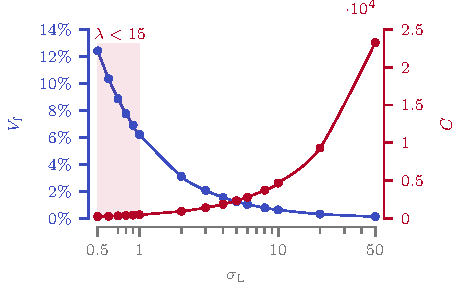
\includegraphics{figures/03_comparison_TO_TTO/13b_tto_graph_log/tto_c.pdf}}
    \hspace*{\fill}
    \caption{Linear (a) and logarithmic (b) plot of the volume fraction $V_\text{f}$ and the compliance $C$ with respect to the maximum material admissible $\sigma_\text{L}$ for the truss-like structures. Areas in red represent the boundaries of the applied method.}
    \label{fig:03_tto_plot}
\end{figure*}

\subsection{Discussion}
In this section, we present a series of graphs for the two formulations comparing the three figures of merit that have been considered thus far: the maximum material admissible $\sigma_\text{L}$, the compliance $C$, and the volume fraction $V_\text{f}$. It's important to note that the data presented in these graphs excludes the values that fall outside the limits highlighted for the two different discretizations in the previous subsections.
\begin{figure}
    \centering
    \includegraphics{figures/03_comparison_TO_TTO/14_stress_comp/stress_comp.pdf}
    \caption{Compliance -- Maximum material admissible plot for the continuous and truss discretizations.}
    \label{fig:03_stress_comp}
\end{figure}

\figref{fig:03_stress_comp} depicts the stress compliance graph for the L-shaped beam load case under consideration. It is evident that the truss configuration consistently exhibits lower compliance values for every considered material admissible and maintains a perfectly linear relationship, in contrast to the continuous discretization approach. We speculate that the difference may be attributed to the non-linearity of the formulation, potentially causing the continuous approach to converge to a local minimum.

In \figref{fig:03_stress_vol} we plot the different volume fractions obtained for a given material admissible (the axis in the graph are swapped as for us the most important figure of merit is the volume fraction).
\begin{figure}
    \centering
    \includegraphics{figures/03_comparison_TO_TTO/15_stress_vol/stress_vol.pdf}
    \caption{Maximum material admissible -- Volume fraction plot for the continuous and truss discretizations.}
    \label{fig:03_stress_vol}
\end{figure}
The continuous mesh yields structures that are more massive for a given material limit. This outcome can be attributed not only to the aforementioned non-linearity in the formulation but also to another intriguing phenomenon. When dealing with volumes exceeding \qty{1}{\percent} (see \figref{fig:03_to_sol}b), we observe that the material in the topology-optimized structure is distributed across multiple elements, appearing somewhat “smeared”. In contrast, the truss representation concentrates all the structural mass along an imaginary line extending from one node to another, being more efficient.

We can also distinctly observe that the truss representation serves as the lower limit of the topology optimization for low volume fractions. Interestingly, both discretizations follow a similar trend for high-volume fractions, despite the significant disparity in their physical description models. The very same trends can be observed watching the volume-complaince graph of \figref{fig:03_comp_vol}.
\begin{figure}
    \centering
    \includegraphics{figures/03_comparison_TO_TTO/16_comp_vol/comp_vol.pdf}
    \caption{Compliance -- Volume fraction plot for the continuous and truss discretizations.}
    \label{fig:03_comp_vol}
\end{figure}

Finally, in \figref{fig:03_time_vol} we turn our attention to the time comparison between the two optimization methods. It is noteworthy that a consistent three-order of magnitude difference is observed between the two methods (days vs. minutes). Additionally, it's worth recalling that in the truss case, employing an extremely fine ground structure is not a necessity, which implies that the time difference could potentially be even bigger.

\begin{figure}
    \centering
    \includegraphics{figures/03_comparison_TO_TTO/17_time_vol/time_vol.pdf}
    \caption{Time -- Volume fraction plot for the continuous and truss discretizations.}
    \label{fig:03_time_vol}
\end{figure}

The notable difference in computation time for stress-based topology optimization (which is not self-adjoint in contrast to compliance minimization) points to the potential for exploring \gls{sand} topology optimization. While preliminary studies in this direction have been conducted~\sidecite{munro_local_2017}, they lie beyond the scope of this thesis and will not be further investigated. It's worth mentioning that \gls{sand} approaches typically lead to a substantial increase in the number of design variables. However, in truss topology problems, this is less of a concern due to the ground structure approach, which results in numerous cross-sectional area design variables and fewer displacement-related ones. This, however, does not hold when dealing with a continuous mesh.

To sum up, in comparing truss and continuous discretization methods, the advantages of truss structures become evident when considering the limitations of continuous discretization for the optimization of ultralight structures. One key drawback of continuous discretization is its increasing need for more elements as the desired level of refinement becomes finer at low volume fractions. Additionally, continuous discretization faces challenges with stress limits in optimized structures, which often exceed the specified admissible limits. Strategies exist to address this issue, but they come at the cost of increased computation time. Furthermore, stress constraints in continuous discretization are often defined for equivalent Von Mises stress, making it more challenging to distinguish between asymmetric bounds for tension and compression. Finally, truss structures are naturally subject to local buckling as a mode of failure~\sidecite{sigmund_non-optimality_2016}, a phenomenon that can be more easily and directly modeled in a truss discretization. 

While truss discretization offers advantages in terms of computational efficiency, it does come with certain limitations. In the minimum volume formulation, the problem is linear and cost-effective to solve. However, the linearity is lost when additional constraints, such as local buckling, are introduced. Moreover, the formulation does not inherently account for the kinematic compatibility of the problem. This limitation restricts its applicability to relatively simple problems and can pose issues when dealing with complex scenarios involving multiple loads or constraints that may lead to structures that are statically indeterminate.

Despite these challenges, we decided to favor truss discretization for our research. In the upcoming chapter, we will address and explore potential solutions to address its main limitations to further enhance its applicability and effectiveness.

\section{Conclusion}
Since the first developments of the topology optimization method, it has been recognized that "For moderately low volume fractions the lay-out of truss-like structures is predicted, but for very low volume fractions it is recommended that the traditional lay-out theory be employed..."~\sidecite{bendsoe_optimal_1989}. However, the performance gap has never been quantified, nor has the domain of applicability been assessed. This is the primary motivation behind this chapter. Additionally, it's important to note that these assumptions were primarily based on compliance formulations and not on volume minimization formulations, which are more pertinent to the aeronautical context.

In this chapter, we introduced a volume minimization formulation applicable to both continuous and truss-like discretizations, aiming at a meaningful comparison. We established a standardized two-dimensional test case, the L-shaped beam, commonly used in stress-based optimization. We conducted multiple optimization runs for both discretization methods using various materials and subsequently compared the results, focusing primarily on volume fraction, compliance, and stress in the optimized structures.

Considering the limitations encountered with the continuous approach, particularly at very low volume fractions, we opted for the truss discretization method for our specific research problem. We also identified certain limitations inherent to truss discretizations, which will be addressed in the following chapter.

% \setchapterpreamble[u]{\margintoc}
\glsresetall % reset glossary
\chapter{Enriching the classic TTO formulation with advanced mechanical constraints}

Chapter 3 highlighted some inherent limitations of the truss modeling and the conventional optimization formulation of \gls{tto}. These limitations include the minimum slenderness problem and the absence of local buckling and kinematic compatibility constraints. The primary objective of this chapter is to propose a comprehensive formulation capable of addressing these shortcomings. As we will observe, the resulting formulation, if solved in its original form, tends to yield solutions characterized by numerous active and intersecting bars. To mitigate this, we propose a two-step optimization algorithm that offers a means to reduce the solution complexity. Additionally, we introduce a heuristic designed to reduce the influence of the starting point within this two-step optimization algorithm. \marginnote{Part of the content presented in this chapter has been published \todo{finish}.}

In \secref{sec:04_constr}, we detail and model the various mechanical constraints applied in the context of \gls{tto}. Subsequently, in \secref{sec:04_formulation_and_algo}, a comprehensive formulation is presented along with an accompanying optimization algorithm. Through the utilization of this optimization algorithm, we are able to maintain control over the complexity of the design. Finally, in \secref{sec:04_numerical_app}, we put the proposed formulation to the test, applying it to various 2D and 3D test cases sourced from the literature, as well as novel cases. The objective is to assess its capabilities and numerical performance.

\section{Advanced mechanical constraints} \label{sec:04_constr}
This section aims to introduce additional mechanical constraints that will be utilized in this study, to reduce the need for post-processing at the end of the optimization process, just before the manufacturing phase begins. We begin by addressing the issue of minimum slenderness, a side constraint that is imposed on the cross-sectional area of the active members to guarantee that the solution adheres to the truss modeling. Subsequently, we address the local buckling constraints, a critical failure mode observed in ultra-light truss structures. Particular attention is devoted to examining the stability of nodes within what are known as compressive chains. The combination of local buckling and nodal stability, a phenomenon known in the literature as topological buckling, is discussed. Furthermore, as we want our formulation to be as versatile as possible, we explore the extension of these constraints to accommodate multi-load cases. A challenge arises from the fact that the resulting structures are frequently statically indeterminate. To address this, we introduce an additional mechanical constraint known as "kinematic compatibility" to ensure that the predicted force field aligns with the displacements of the structure.

\begin{table*}
    \centering
    \resizebox{\columnwidth}{!}{%
    \begin{tabular}{
        V{5cm}
        V{2.5cm}
        V{1.7cm}
        V{2.5cm}
        V{2.2cm}
        V{2.5cm}
        V{2cm}}
        \toprule
    Authors &
      Stress &
      Local Buckling &
      Topological buckling &
      Kinematic compatibility &
      Multi-load cases &
      Minimum slenderness
       \\ \midrule
    Dorn et al. (1964)  \cite{dorn_automatic_1964}                & x &-&-&-&-&-\\
    Hemp (1973)  \cite{hemp_optimum_1973}                       & x &-&-&-& x &-\\
    Reinschmidt et al.   (1974) \cite{reinschmidt_applications_1974}         & x & x &-& $\sim$ &-&-\\
    Kirsch (1980) \cite{kirsch_optimal_1980}                       & x &-&-& x &-&-\\
    Oberndorfer et al. (1996)   \cite{oberndorfer_two_1996}        & x & x &-&-&-&-\\
    Silva Smith (1997)  \cite{silva_smith_topology_1997}                & x & x & $\sim$ &-& x &-\\
    Achtziger (1999a, 1999b) \cite{achtziger_local_1999,achtziger_local_1999b}            & x & x & x &-& x &-\\
    Stolpe (2004)   \cite{stolpe_global_2004}                    & x & x &-& x & x &-\\
    Pritchard et al. (2005)  \cite{pritchard_plastic_2005}           & x &-&-&-& x &-\\
    Tyas et al. (2006)   \cite{tyas_practical_2006}               & x & x & x &-& x &-\\
    Descamps et al. (2014)  \cite{descamps_nominal_2014}            & x & x & x &-& x &-\\
    Schwarz et al. (2018) \cite{schwarz_efficient_2018}              & x & x &-&-&-&-\\
    Cai et al. (2022)  \cite{cai_topology_2022}                 & x & x & x &-&-&-\\
    Present work                        & x & x & x &x&x&x\\ \bottomrule
    \end{tabular}}
    \caption{Non-exhaustive list of the existing research in Truss Topology Optimization (TTO) with their corresponding scientific contributions.}
    \label{tab:04_literature}
\end{table*}

In \tabref{tab:04_literature}, we provide an overview of historical and contemporary research in the field of \gls{tto}, along with their respective scientific contributions. This serves to highlight the necessity for a more comprehensive formulation that incorporates these mechanical constraints, reducing the gap between the optimized design and the actual manufactured structure.
    
\subsection{Minimum slenderness constraints}
As previously discussed in \secref{sec:03_applications}, the \gls{tto} method shows numerous limitations due to its reliance on the truss model. Therefore, the resulting structures may not be acceptable if the model falls outside the bounds of this idealization. To better study this limit, as outlined in \secref{sec:03_applications}, we introduced a metric called bar slenderness, which is defined as follows:
\begin{equation}
    \lambda = \frac{\ell}{R_{\mathrm{g}}},
\end{equation}
where $R_{\mathrm{g}}$ represents the gyration radius of the cross-sectional area, defined as $R_{\mathrm{g}} = \sqrt{I/a_j}$.
The primary objective of this section is to introduce an upper limit constraint on the cross-sectional area design variable. This constraint prevents a bar from exceeding the bounds of its idealized model, thereby enhancing the optimization process's robustness.

Remembering that for a circular cross-section $I = \pi r_j^4/4$, we can write
\begin{equation}
    R_{\mathrm{g},j} = \frac{r_j}{2}.
\end{equation}
The minimum slenderness limit constraints are then stated as:
\begin{equation} \label{eq:04_slend_constraints}
    a_j \leq \frac{4 \pi \ell_j^2}{\lambda_{\text{max}}}, \quad \forall j \in [1,\ldots, N_{\text{el}}]
    \tag{$\vect{g}_{\text{slend}}$}
\end{equation}
for a fixed $\lambda_{\text{max}}$. In this thesis we set $\lambda_{\text{max}}=15$.

\subsection{Local and topological buckling constraints}
Adding local buckling constraints to the optimization formulation is fundamental, as ultralight truss structures are often dominated by this mode of failure \sidecite{sigmund_non-optimality_2016}. By imposing local buckling constraints over a \gls{tto} problem (where the lower bound for the members' cross-sectional areas is 0), the optimization domain becomes disjointed \sidecite{cheng_aspects_1995}. The solution is to be searched inside a degenerate space of the design space of the optimization, known in the literature as singular optimum \sidecite{guo_new_2001}. Stolpe \sidecite{stolpe_note_2003} showed how using the \gls{sand} formulation with local buckling and kinematic compatibility constraints, it is possible to find well-optimized structures without the use of relaxation techniques. The authors, however, point out how the solution is still very sensitive to the initialization point of the \gls{nlp} formulation. The local buckling constraints $\vect{g}_{\text{buck}}$ are stated using Euler's critical load formula as:
\begin{equation}
    q_j  + \frac{s_j a_j^2}{\ell_j^2} \geq 0 \quad \forall j \in [1,\ldots, N_{\text{el}}],
    \tag{$\vect{g}_{\text{buck}}$}
    \label{eq:04_buck}
\end{equation}
where $s_j$ is a parameter dependent on the member material and section topology as follows:
\begin{equation}
    s_j=\pi^2 E \beta_j.
    \label{eq:04_s}
\end{equation}
$\beta_j=I_j/a^2_j$ is a positive constant dependent on the moment of inertia and the section of the $j$-th bar, and $E$ is Young's modulus of the material. Assuming that the shape of the cross-section is identical over the whole structure and is independent of $a$, it follows that  $\beta_j = \beta$ and $s_j = s, \; \forall j \in [1,\ldots, N_{\text{el}}]$.

Direct application of the local buckling constraint \eqrefnotext{eq:04_buck} in the optimization formulation tends to create "chains" of unstable compressive members \sidecite{bendsoe_optimization_1995, zhou_difficulties_1996, rozvany_difficulties_1996}. This problem is known in the literature as topological buckling \sidecite{achtziger_local_1999}, as the definition of the compressive chains is a function of the topology of the structure, and is one of the elements of the nodal stability of the structure. Additional forms of structure instability, such as global buckling \sidecite{ben-tal_optimal_2000,kocvara_modelling_2002, neves_generalized_1995, ferrari_topology_2021} or the use of lateral perturbing forces to obtain nodal stability \sidecite{tyas_practical_2006,mela_resolving_2014} have been studied in the literature. However, since they are beyond the scope of this work, they will not be discussed further.

\begin{figure}
    \centering
    \includegraphics{figures/04_TTO_improvements/01_3_bars_chain/3_bars_chain.pdf}
    \caption{The three ground structures loaded in compression are used to highlight the topological buckling problem in \gls{tto}. (a) Two-bar ground structure loaded in compression; (b) single bar ground structure; (c) overlap of the $a$ and $b$ ground structures.}
    \label{fig:04_chain_buck}
\end{figure}

To illustrate the topological buckling phenomenon, we consider the case shown in \figref{fig:04_chain_buck}a. It consists of a ground structure with $M=3$ nodes and $N_{\text{el}}=2$ bars with length $\ell_1=\ell_2=\ell$, and a compressive load of magnitude $F$ applied at the right-hand side node. For this trivial structure, we can state that $q_1=q_2=F$ and thus $a_1=a_2=a$. We suppose here that the allowables of the material are such that the local buckling (and not the stress) is the most limiting failure criterion for the bars. Assuming that the shape of the section is equal, the local buckling constraints are written as:
\begin{equation}
    q_j\geq -\frac{s a^2}{\ell^2}, \quad j\in[1,2].
    \label{eq:04_chain_1}
\end{equation}
However, the structure is unstable because the vertical force equilibrium equation evaluated on the central hinge is satisfied only in an ideal case where no structural imperfections are taken into account.

If the hinge between bars 1 and 2 is deleted, we obtain the structure pictured in \figref{fig:04_chain_buck}b with $\ell_3=2\ell$. The local buckling constraints for bar 3 are thus:
\begin{equation}
    q_3\geq -\frac{s a_3^2}{(2\ell)^2}.
    \label{eq:04_chain_2}
\end{equation}

Combining \eqsref{eq:04_chain_1}, \eqrefnotext{eq:04_chain_2} and observing that $q_1=q_2=q_3=F$, it is now trivial to demonstrate that $a_3=2a$. Constraint \eqrefnotext{eq:04_chain_2} leads, then, to more voluminous structures compared to constraint \eqrefnotext{eq:04_chain_1}. For that reason, even if we consider the ground structure given in \figref{fig:04_chain_buck}c composed by the superposition of the ground structures in \figref{fig:04_chain_buck}a and \figref{fig:04_chain_buck}b, the optimization with a uniform initialization tends to converge to the solution $\vect{a}^*=[a,a,0]$, unstable but lighter than the physical solution $\vect{a}_p^*=[0,0,2a]$. 

The easiest way to get rid of the instability of the compressive chains is to post-process the optimized structure and remove the unstable hinges between the compressive bars. Doing that, the local buckling constraints are not satisfied anymore as the effective buckling length has increased. It is, then, necessary to calculate the section of the new compressive bars to comply with the newly introduced buckling constraints. As extensively shown by Achtziger \sidecite{achtziger_local_1999b}, this post-processing phase leads to structures that are less optimal compared to the ones we could obtain if we take into account the topological buckling in the optimization in the first place.

For that reason, Achtziger proposes an update strategy to modify the length used to evaluate the critical buckling force of \eqrefnotext{eq:04_buck} as follows:
\begin{equation}
    \ell^*_j(\vect{a}):= 
    \begin{cases}
        \ell_j & \text { if } j \notin \mathcal{C}_{l,r}(\vect{a}) \\
        \sum \ell_{r} \;|\; r \in \mathcal{C}_{l,r}(\vect{a})  & \text { otherwise,}
    \end{cases}
    \label{eq:04_chain_len}
\end{equation}
where $r$ represents the $r$-th bar of the $l$-th compression chain of the structure. The topology-dependent set $\mathcal{C}_{l,r}(\vect{a})$ is defined as the set of $r$ member indexes of the $l$-th buckling chain. As internal forces on buckling chains are constant, only the buckling length of the first member of the chain ($\ell^*_j(\vect{a}) \text{ with } j \in \mathcal{C}_{l,1}(\vect{a})$) is modified. Additionally, we add the following side constraints on the other members of the $l$-th chain to ensure feasibility:
\begin{equation}
    a_{r}\geq a_{r=1} \quad \; r \in \mathcal{C}_{l,r}(\vect{a}), \; \forall r \neq 1.
    \label{eq:04_side_cons_chain}
\end{equation}

\subsection{Kinematic compatibility constraints}
To optimize test cases that result in statically indeterminate structures, such as structures loaded with multiple load cases or imposed symmetries, we add an additional mechanical constraint called kinematic compatibility \sidecite{kirsch_optimal_1989, rozvany_layout_1995}. Compatibility can be imposed as a nonlinear constraint in the optimization formulation \sidecite{kirsch_optimal_1980}, or can be taken into account by prestressing the initial structure \sidecite{kirsch_effect_1989}.

The kinematic compatibility constraints restrict the displacement field $\vect{U} = [U_1, \ldots,U_{N_{\text{dof}}}]^T$ in such a way that strains $\varepsilon_j$ and internal stresses $\sigma_j$ comply with Hooke's law $\sigma_j = E_j \varepsilon_j$ with $j \in [1,\ldots, N_{\text{el}}]$. Recalling that in a truss the relationship between nodal displacements and member deformations is $\vect{b}^T_j \vect{U} = \ell_j \varepsilon_j$ with $\vect{b}$ as the $j$-th column of the $\matr{B}$ matrix, we can formulate the kinematic compatibility constraints $\vect{g}_{\textrm{comp}}$ as:
\begin{equation}
\label{eq:04_compatib}
     q_j - \frac{a_j E_j}{\ell_j} \vect{b}_j^T\vect{U}  = 0  \quad \forall j \in [1,\ldots, N_{\text{el}}].
     \tag{$\vect{g}_{\textrm{comp}}$}
\end{equation}
Kinematic compatibility constraints are non-linear as the design variable $\vect{q}$ is dependent on $\vect{a}$ and $\vect{U}$.


\section{Optimization formulation and solving strategy} \label{sec:04_formulation_and_algo}
\label{sec:04_method}
In this section, we propose an innovative \gls{tto} formulation developed specifically to minimize the mass of 3D ultralight truss structures, taking into account maximum stress, topological buckling, kinematic compatibility, and minimum slenderness constraints. Combining Formulation \eqrefnotext{eq:03_optim_original} with \eqsref{eq:04_buck} \eqrefnotext{eq:04_slend_constraints}, \eqrefnotext{eq:04_chain_len}, \eqrefnotext{eq:04_side_cons_chain}, and \eqrefnotext{eq:04_compatib}, Formulation $\mathbb{P}_1$ is stated in terms of members' cross-sectional area $\vect{a}$, member forces $\vect{q}$ and nodal displacements $\vect{U}$ as follows:
\begin{equation}
    \begin{aligned}
    \underset{\vect{U}^0, \dots, \vect{U}^{N_p}}{\min_{\vect{a}, \vect{q}^0, \dots, \vect{q}^{N_p},}}   && V &= \vect{\ell}^{T}\vect{a}\\
    \textrm{s.t.}   && \matr{B}\vect{q}^p &= \vect{f}^p && \forall p \in [0,\dots,N_p]\\
    && \vect{q}^p &= \frac{\vect{a}E}{\vect{\ell}}\vect{b}^T\vect{U}^p && \forall p \in [0,\dots,N_p] \\
    && \vect{q}^p &\geq -\frac{s\vect{a}^2}{\vect{\ell}^{*2}} && \forall p \in [0,\dots,N_p] \\
    && -\sigma_\text{c}\vect{a} &\leq \vect{q}^p \leq \sigma_\text{t}\vect{a} && \forall p \in [0,\dots,N_p] \\
    && a_{r}&\geq a_{r=1} && r \in \mathcal{C}_{l,r}(\vect{a}) \\
    && 0 &\leq \vect{a} \leq \frac{4 \pi \vect{\ell}^2}{\lambda_{\text{max}}}. \\
    \end{aligned}
    \tag{$\mathbb{P}_1$}
    \label{eq:04_optim_complete}
\end{equation}
The formulation has been extended to multiple load cases given by $N_p$ external loads vector $\vect{f}^0, \dots, \vect{f}^{N_p}$ and the resulting internal forces $\vect{q} = [\vect{q}^0,\dots, \vect{q}^{N_p}]$ and displacements $\vect{U} = [\vect{U}^0,\dots, \vect{U}^{N_p}]$. This proposed formulation expands the multiple load cases formulation of Achtziger \sidecite{achtziger_local_1999} with kinematic compatibility constraints, permitting the correct evaluation of the mechanical state of statically indeterminate structures.

The formulation follows the \gls{sand} approach \sidecite{sankaranarayanan_truss_1994}, where, in addition to the members' cross-sectional area $\vect{a}$, the member forces $\vect{q}$ and the structure displacements $\vect{U}$ are used as state variables. One of the advantages of \gls{sand} approach is that the state variables are independent of each other and, thus, the sensitivity calculation of the constraints functions is usually simpler and leads to sparse partial derivatives. Additionally, compared to \gls{nand} formulations, the problem stays well-posed even if the cross-sectional area goes to 0. As the linear system $\matr{K}\vect{U}=\vect{f}$ is never explicitly solved during the optimization, it is not necessary to impose a lower bound on the members' cross-sectional area $\vect{a}$ to avoid a singular stiffness matrix. The last important advantage is that thanks to $\vect{U}$ being design variables, it is trivial to add bound constraints on the nodal displacements of the structure if needed.

\subsection{Optimization strategy} \label{sec:04_2step_opt}
Formulation \eqrefnotext{eq:04_optim_complete} presents multiple constraints and design variables for every physical bar of the ground structure. The quantity of constraints creates a highly non-linear design space and it proved to be hard for the optimizer to bring to zero the value of the cross-sectional areas. If a \gls{nlp} optimizer is directly used on Formulation \eqrefnotext{eq:04_optim_complete}, the resulting structure will be composed of a multitude of intersecting bars. The optimizer is, thus, working like it is performing sizing optimization instead of topology optimization. 

Inspired by the early works by Reinschmidt \sidecite{reinschmidt_applications_1974}, we propose a novel two-step optimization strategy in which a first optimization solving a relaxed formulation is used to find a good starting point for the second optimization, solving the full Formulation \eqrefnotext{eq:04_optim_complete}. Doing that way, the first optimization explores extensively the relaxed and more regular design space and finds simpler structures, while the second optimization refines the solution imposing additional mechanical constraints. The complete solving strategy is graphically presented in \figref{fig:04_sol_alg}.

In the first step, Problem \eqrefnotext{eq:04_optim_complete} is relaxed: kinematic compatibility constraints are omitted. We call this relaxed Problem $\mathbb{P}_2$. Problem $\mathbb{P}_2$ is solved using a \gls{slp} method by iteratively linearizing the local buckling constraints. A heuristic strategy called Reinitialization is iteratively used to reduce the influence of the starting point $\vect{a}_0$. The resulting structure described by the design variables vector $\vect{\tilde{x}}^*$ is then post-processed, removing the members whose optimized area is below a fixed cross-sectional area threshold value. The structures generated by solving the relaxed Problem $\mathbb{P}_2$ proved to be simpler \ie fewer active members compared to directly solving \eqrefnotext{eq:04_optim_complete} with a \gls{nlp} optimizer. If the solution is not statically indeterminate the optimization is completed as the kinematic compatibility constraints \eqrefnotext{eq:04_compatib} are automatically satisfied and, thus, used to evaluate the optimal displacements.

Otherwise, a second step is needed. Firstly, the ground structure of the problem is simplified, removing all the members that do not appear in the solution of the relaxed Problem $\mathbb{P}_2$ \ie avoiding the reintroduction of members discarded by the \gls{slp} step. Then, the kinematic compatibility and the exact local buckling constraints are restored, and Problem \eqrefnotext{eq:04_optim_complete} is solved in its original form on the simplified ground structure using a \gls{nlp} optimizer. The initial values for the cross-sectional areas are the solution $\vect{\tilde{x}}^*$ of Problem $\mathbb{P}_2$.

\begin{figure*}
    \centering
    \includegraphics[width=\linewidth]{figures/04_TTO_improvements/02_solution_algo/sol_algo.pdf}
    \caption{Flowchart of the two-step optimization strategy used to solve Problem \eqrefnotext{eq:04_optim_complete}.}
    \label{fig:04_sol_alg}
\end{figure*}

\subsection{First step: SLP optimization}
The first step of the proposed optimization strategy is here described in detail. The relaxed Problem $\mathbb{P}_2$ obtained by omitting \eqrefnotext{eq:04_compatib} and the displacements $\vect{U}$ in Formulation \eqrefnotext{eq:04_optim_complete} is stated as:
\begin{equation}
    \begin{aligned}
    \min_{\vect{a}, \vect{q}^0, \dots, \vect{q}^P}  && V &= \vect{\ell}^{T}\vect{a}\\
    \textrm{s.t.}   && \matr{B}\vect{q}^p &= \vect{f}^p && \forall p \in [0,\dots,N_p]\\
    && \vect{q}^p &\geq -\frac{s\vect{a}^2}{\vect{\ell^{*2}}} && \forall p \in [0,\dots,N_p] \\
    && -\sigma_\text{c}\vect{a} &\leq \vect{q}^p \leq \sigma_\text{t}\vect{a} && \forall p \in [0,\dots,N_p] \\
    && a_{r}&\geq a_{r=1} && r \in \mathcal{C}_{l,r}(\vect{a}) \\
    && 0 &\leq \vect{a} \leq \frac{4 \pi \vect{\ell}^2}{\lambda_{\text{max}}}. \\
    \end{aligned}
    \tag{$\mathbb{P}_2$}
    \label{eq:04_optim_no_constr}
\end{equation}

Since the objective function and all of its constraints are linear, except for the buckling constraint, this problem is solved by iteratively linearizing the non-linear buckling constraints and using a \gls{slp} algorithm. Following the work of \sidecite{schwarz_efficient_2018}, the Euler's critical load is iteratively updated using a first-order Taylor expansion for every $j$ member with cross-sectional area $a_{j}^i$ at the iteration $i$ in the neighborhood of the point $\vect{P}_{i}$ (see \figref{fig:04_SLP}):
\begin{equation}
    \tilde{q}_{i,j}^{\text{cr}} = q_{i,j}^{\text{cr}}(a_{j}^i) + (a_{j}^{i+1} - a_{j}^i)\left.\derfrac{q_{i,j}^{\text{cr}}(a_{j}^i)}{a}\right\rvert_{a=a_{j}^i}
\end{equation}
where $a_{j}^{i+1}$ represent the design variable of the \gls{slp} at the current iteration and $q^{\text{cr}}_{i,j}(a_{j}^i) = -s ({a_{j}^i})^2/\ell^{*2}_j$ represents the Euler's critical load with cross-sectional area $a_{j}^i$ and modified buckling length $\ell^{*}_j$. 

The linearized local buckling constraints $\vect{\tilde{g}}_{\textrm{buck}}$ are then stated as:
\begin{equation}
    q_{j} \geq \tilde{q}^{\text{cr}}_{i,j},\text{ with } \tilde{q}^{\text{cr}}_{i,j}= - \frac{s a_{j}^i\left(2 a_{j}^{i+1} - a_{j}^i\right)}{\ell^{*2}_j} \quad \forall j \in [1,\ldots, N_{\text{el}}],
    \label{eq:04_buck_con_lin}
    \tag{$\vect{\tilde{g}}_{\textrm{buck}}$}
\end{equation}
where superscript $\sim$ indicates linearized functions and corresponding variables.

\begin{figure}
    \centering
    \includegraphics[width=0.7\linewidth]{figures/04_TTO_improvements/03_SLP/slp.pdf}
    \caption{Linearization of the local buckling constraints for a single bar.}
    \label{fig:04_SLP}
\end{figure}


We can now state the relaxed linearized sub-problem $\tilde{\mathbb{P}}_2$ obtained substituting \eqrefnotext{eq:04_buck} with \eqrefnotext{eq:04_buck_con_lin} in Formulation \eqrefnotext{eq:04_optim_no_constr}:
\begin{equation}
    \begin{aligned}
    \min_{\vect{a}, \vect{q}^0, \dots, \vect{q}^P}   && V &= \vect{\ell}^{T}\vect{a}\\
    \textrm{s.t.}   && \matr{B}\vect{q}^p &= \vect{f}^p && \forall p \in [0,\dots,N_p]\\
    && \vect{q}^p \geq - &\frac{s \vect{a}^i\left(2 \vect{a}^{i+1} - \vect{a}^i\right)}{\vect{\ell}^{*2}} && \forall p \in [0,\dots,N_p] \\
    && -\sigma_\text{c}\vect{a} &\leq \vect{q}^p \leq \sigma_\text{t}\vect{a} && \forall p \in [0,\dots,N_p] \\
    && a_{r}&\geq a_{r=1} && r \in \mathcal{C}_{l,r}(\vect{a}) \\
    && 0 &\leq \vect{a} \leq \frac{4 \pi \vect{\ell}^2}{\lambda_{\text{max}}}. \\
    \end{aligned}
    \tag{$\tilde{\mathbb{P}}_2$}
    \label{eq:04_optim_no_constr_lp}
\end{equation}

Since the objective function and all of its constraints are linear, we can approximate the solution of \eqrefnotext{eq:04_optim_no_constr} by iteratively solving the sub-problem \eqrefnotext{eq:04_optim_no_constr_lp}. At every iteration $i$, the vector of cross-sectional areas $\vect{a}^i$ is used to evaluate the linearization point $\vect{P}_{i}$ and calculate the set of linearized buckling constraints $\vect{\tilde{g}}_{\textrm{buck}}$ (see \figref{fig:04_SLP}). The sub-problem \eqrefnotext{eq:04_optim_no_constr_lp} is, then, solved using a \gls{lp} solver, and the updated vector of cross-sectional areas $\vect{a}^{i+1}$ is used to evaluate the set of linearized buckling constraints of the $i+1$ iteration. These steps are repeated until convergence \ie when $\norm{\Delta \vect{x}}_\infty\leq \text{tol}_{slp}$, where $\Delta \vect{x}$ represents the difference of the design variable vector $\vect{x}$ between two successive iterations. The vector $\vect{x}$ is scaled so that the difference $\Delta \vect{x}$ gives coherent results for the different physical quantities (cross-sectional areas and forces).

\subsection{Handling local minima: reinitialization strategy}
\label{sec:04_reinit}

% \begin{figure*}
%     \centering
%     \subcaptionbox{\label{fig:04_tiny-area}}{\includegraphics[width=0.45\linewidth]{figures/04_TTO_improvements/04_SLP_tiny_area_design_space/slp_tiny_design_space.pdf}}
%     \bigskip
%     \subcaptionbox{\label{fig:04_reinit_strat}}{\includegraphics[width=0.45\linewidth]{figures/04_TTO_improvements/05_reinit_strategy/reinit_strat.pdf}}
%     \caption{(a) ; (b) }
% \end{figure*}
\begin{marginfigure}
    \centering
    \includegraphics[width=\linewidth]{figures/04_TTO_improvements/04_SLP_tiny_area_design_space/slp_tiny_design_space.pdf}
    \caption{The linearized buckling constraints (blue dashed line) limit the design space of successive iterations when evaluated on compressive bars with very small areas. Additionally, the gradient of the linearized buckling constraint tends to 0.}
    \label{fig:04_tiny-area}
\end{marginfigure}

\begin{figure}
    \centering
    \includegraphics[width=0.7\linewidth]{figures/04_TTO_improvements/05_reinit_strategy/reinit_strat.pdf}
    \caption{The reinitialization strategy modifies the linearization point of the members with a small area to promote their reintroduction in the optimization problem.}
    \label{fig:04_reinit_strat}
\end{figure}

If at the end of iteration $i-1$ the cross-sectional area of bar $j$, $\vect{a}^i_{j}$, becomes very small, the gradient of the corresponding local buckling constraint at iteration $i$ will tend towards 0 and the feasible domain will be extremely reduced (see \figref{fig:04_tiny-area}). Any bar with near-zero sections will remain as such in future iterations since there is no incentive for the \gls{slp} optimizer to increase its value. This is one of the possible reasons why the \gls{slp} optimizer gets stuck in local minima.

Subsequently, we propose a heuristic strategy to reinitialize the small cross-sectional area values $\vect{a}^{i}$ used to evaluate the linearized local buckling constraints $\tilde{g}_{\text{buck}}$ at iteration $i$. The strategy is called $k$ times during the optimization when the solver converges to a minimum, \ie when $ \norm{\Delta \vect{x}}_\infty \leq \text{tol}_{slp} $. It affects only the cross-sectional areas that are smaller than a fraction value $\tau$ of the maximum value at iteration $i$, $\norm{\vect{a^i}}_\infty$. The updated cross-sectional area $\overline{\vect{a}}^i$ used to evaluate the linearization point $\overline{\vect{P}}_{i}$ is updated as follows:
\begin{equation}
    \overline{a}^i_{j}:=
    \begin{cases}
        \phi_k \norm{\vect{a^i}}_\infty & \text{ if } a^i_{j} \leq \tau \norm{\vect{a^i}}_\infty\\
        a^i_{j} & \text { otherwise.}  
    \end{cases}
    \label{eq:04_reinit}
\end{equation}
The effects of this approach are shown in \figref{fig:04_reinit_strat}, where it is clear that updating the constraint $\tilde{g}_{\text{buck}}$ with $\overline{\tilde{g}}_{\text{buck}}$ reduces the gap between the original and the linearized design space and permits the exploration of new solutions. Additionally, the gradient of the constraint is restored to a non-zero value.

\begin{figure}
    \centering
    \includegraphics[width=0.7\linewidth]{figures/04_TTO_improvements/06_SLP_algo/SLP_algo.pdf}
    \caption{Flowchart of the \gls{slp} strategy with reinitialization used to solve Problem \eqrefnotext{eq:04_optim_no_constr}.}
    \label{fig:04_slp_solution}
\end{figure}

The $\phi_k$ parameter is used in \eqref{eq:04_reinit} to influence how much the reinitialization heuristic modifies the original formulation. Subsequently, to reach convergence, we propose a continuation scheme on $\phi_k$ to reduce its impact on the optimization following an exponential decay law:
\begin{equation}
    \phi_k = \phi_{k-1}^\beta \quad \forall k \in [1,\dots,k_{\text{max}}],
    \label{eq:04_phi}
\end{equation}
where $k_{\text{max}}$ represent the maximum number of reinitialization calls and the $\beta$ parameter control the steepness of the exponential progression. In that way, as the number of calls to the reinitialization strategy increases, its influence on the original formulation decreases.

The complete \gls{slp} strategy with reinitialization used to solve Problem \eqrefnotext{eq:04_optim_no_constr} is presented in \figref{fig:04_slp_solution}, where the \gls{slp} optimized design variable vector is noted as $\vect{\tilde{x}}^*=[\tilde{\vect{a}}^*, \; \tilde{\vect{q}}^*]$.

\subsection{Second step: NLP optimization}
If only one load case and no particular symmetries are imposed on the initial ground structure, the \gls{slp} solution $\vect{\tilde{x}}^*$ is not statically indeterminate \sidecite{kirsch_optimal_1989, rozvany_layout_1995}. In that case, it is trivial to evaluate the displacements using \eqrefnotext{eq:04_compatib} and the optimization is complete. However, if this is not the case, the stability of the structure is to be tested. 

The stability of the \gls{slp}-optimized structure is assessed by evaluating the \gls{dsi} of the truss using Maxwell's criterion:
\begin{equation}
    DSI= N_{\text{el}} - N_{\text{DOF}} - r
\end{equation}
with $r$ the number of fixed \gls{dofs} of the test case. If $\text{DSI}\leq0$, the number of equilibrium equations is less than or equal to the number of the internal forces and Equation \eqrefnotext{eq:04_compatib} suffices to evaluate the correct displacements of the truss. If, however, $\text{DSI}>0$, the truss is potentially statically indeterminate and additional non-linear constraints must be added to ensure the structure's kinematic compatibility. The optimization is then performed again. We call this second step the \gls{nlp} step (see \figref{fig:04_sol_alg}). 

To mitigate the risk of becoming trapped in local minima, the \gls{nlp} optimizer is employed on a reduced design space. The solution $\vect{\tilde{x}}^*$ of the \gls{slp} serves the purpose of simplifying the initial ground structure, thereby eliminating elements from the \gls{nlp} optimization that fall below the specified threshold value $a_{\text{thr}}$:
\begin{equation}
    a_j<a_{\text{thr}} \; \forall j, \text{ with }a_{\text{thr}} = \chi \; \max(\tilde{\vect{a}}^*),
    \label{eq:04_thr}
\end{equation}
with the parameter $\chi$ called the cross-sectional area threshold value.

An elastic \gls{fea} based on the direct stiffness method is performed to provide a correct estimate of forces and displacements caused by the external forces on the solution of Problem \eqrefnotext{eq:04_optim_no_constr} for the initial point of the optimization. The initial displacement vector $\vect{U}^0$ is calculated as the unique solution to:
\begin{equation}
    \vect{f}=\matr{B}^T \matr{q}=\matr{B}^{T} \matr{D} \vect{\epsilon}=\matr{B}^{T} \matr{D} \matr{B} \vect{U}^0=\matr{K} \vect{U}^0.
    \label{eq:04_truss_fem}
\end{equation} 
 where $\matr{K}$ is the stiffness matrix of the truss, defined as $\matr{K}=\matr{B}^{T} \matr{D} \matr{B}$, with $\matr{D}=\operatorname{diag}\left(E (\tilde{\vect{a}}^* + \delta \vect{e}) / \vect{\ell}\right)$, $e =[1,\dots,1]^T$, and $\delta =10^{-12}$. This last term is added as the structures coming from the \gls{slp} step could result in a mechanism with respect to load cases different from the one used for the optimization \sidecite{dorn_automatic_1964}. Then the initial member forces vector $\vect{q}^0$ is evaluated using \eqrefnotext{eq:04_compatib}. $\tilde{\vect{a}}^*, \vect{q}^0$ and $\vect{U}^0$ are used as the starting point of the full \gls{nlp} formulation where the kinematic compatibility and the exact local buckling formulation are restored. The \gls{nlp} solver finally outputs the optimized structure variables $\vect{x}^*=[\vect{a}^*,\; \vect{q}^*,\; \vect{U}^*]$.

\section{Numerical application} \label{sec:04_numerical_app}
In this section, the proposed method is benchmarked against four classical and innovative test cases. Firstly, we show how the proposed two-step solution strategy with reinitialization reduces the influence of the starting point on the optimization result compared to the direct \gls{nlp} optimization of Problem \eqrefnotext{eq:04_optim_complete}. Additionally, as the response surface of the \gls{slp} of the proposed method is more regular than the original \gls{nlp}, the two-step solution strategy generates simple structures \ie with a low number of active bars, as it is efficient at driving the cross-sectional areas to zero. To show that, we implement and optimize the ten-bar truss and the 2D cantilever beam, two of the most common benchmarks in \gls{tto} with buckling constraints. Secondly, to show the ability of the proposed method to work on structures with multiple load cases we implemented a modified ten-bar truss test case where several load cases are applied to the same ground structure. Finally, to assess the computational efficiency and to validate the proposed strategy on a large-scale structure, we optimize a three-dimensional wingbox test case based on the \acrfull{crm} with multiple discretization refinement.

The test cases are optimized using different resolution strategies. The proposed method is compared against the direct \gls{nlp} optimization of Problem \eqrefnotext{eq:04_optim_complete}, denoted in our analysis as \gls{nlp}. The proposed two-step resolution strategy is implemented with three different maximum numbers of reinitialization calls $k_{\text{max}}$: no reinitialization (2S-0R) with $k_{\text{max}}=0$, one call of reinitialization (2S-1R) with $k_{\text{max}}=1$, and finally five calls of reinitialization (2S-5R) with $k_{\text{max}}=5$. The reinitialization magnitude parameter $\vect{\phi}$ is set up using \eqref{eq:04_phi} and the parameters listed in \tabref{tab:04_param}, leading to $\phi = 0.8000$ for the 2S-1R algorithm and to $\vect{\phi} = \left[ 0.8000, 0.6400, 0.4096, 0.1677, 0.0281 \right]$ for the five reinitialization calls of 2S-5R.

The optimizations are performed using the Python package CVXPY 1.2.2 \sidecite{diamond_cvxpy_2016} with the ECOS 2.0.7 \sidecite{domahidi_ecos_2013} solver to solve the relaxed \gls{lp} Problem \eqrefnotext{eq:04_optim_no_constr_lp}. The \gls{nlp} Problem \eqrefnotext{eq:04_optim_complete} is solved using cyipopt \sidecite{Moore_Mechmotum}, a Python wrapper for IPOPT 3.14.11 \sidecite{wachter_implementation_2006}, a large-scale nonlinear optimization package using PARDISO 6.0 \sidecite{alappat_recursive_2020} as the linear solver. The Jacobian and the Hessian of the Lagrangian of the \gls{nlp} step are calculated at every optimization iteration to allow faster convergence. As every state variable of the optimization is independent of the others, these responses are derived analytically and will not be detailed there. The stopping criterion used for the \gls{slp} and \gls{nlp} optimizations are $\norm{\Delta \vect{x}}_\infty \leq \text{tol}_{slp}  \text{, and } \norm{\Delta_{\text{NLP}}}_\infty \leq \text{tol}_{nlp}$, with $\text{tol}_{slp}=10^{-6}$ and $\text{tol}_{nlp}=10^{-4}$ respectively. $\Delta_{\text{NLP}}$ represents the scaled \gls{nlp} error, a more comprehensive value used by IPOPT to take into account the optimality of the solution and the constraints violation. The objective function is scaled so that the initial volume is 1000, the areas are in the interval $[0,1000]$, the initial forces in $[0,1000]$, and the displacement in $[0,1000]$ for the \gls{slp} and the \gls{nlp}. The full list of parameters used to set up the variable scaling, the \gls{slp} optimization, the reinitialization, and the \gls{nlp} optimization is listed in \tabref{tab:04_param}. Several additional parameters are used in the \gls{nlp} step for cyipopt and IPOPT:
\begin{itemize}
    \item \texttt{mu\_strategy} is set to \texttt{adaptive} 
    \item \texttt{grad\_f\_constant} is set to \texttt{yes} 
    \item \texttt{hessian\_constant} is set to \texttt{yes} 
    \item \texttt{alpha\_for\_y} is set to \texttt{min-dual-infeas}
    \item \texttt{linear\_solver} is set to \texttt{pardiso}
    \item \texttt{expect\_infeasible\_problem} is set to \texttt{yes}
    \item \texttt{bound\_push} is set to \texttt{1e-12}
    \item \texttt{constr\_viol\_tol} is set to \texttt{1e-6}
    \item \texttt{nlp\_scaling\_method} is set to \texttt{user-scaling}.
\end{itemize}

\begin{table}
    \small
\centering
\begin{tabular}{ccc}
\toprule
\textbf{Parameter} & \textbf{Value} & \textbf{Description}    \\ \midrule
$\text{tol}_{slp}$             & $10^{-6}$           & Stopping criterion \gls{slp}                       \\
$\text{tol}_{nlp}$               & $10^{-4}$           & Stopping criterion \gls{nlp}                        \\
max$_{\text{it,SLP}}$        & 400            & Maximum iterations of the \gls{slp} algorithm                       \\
max$_{\text{it,NLP}}$         & 5000           & Maximum iterations of the \gls{nlp} algorithm                        \\
$\chi$                & $10^{-6}$           & Threshold for the ground structure reduction                        \\
$\tau$                & 0.05           & Threshold for the reinitialization                        \\
$\phi_0$              & 0.8            & Initial reinitialization magnitude parameter                         \\
$\beta$             & 2              & Index of the exponential decay law \\
\bottomrule
\end{tabular}
\caption{Values and description of the parameters used for the \gls{slp} and \gls{nlp} optimizations.}
\label{tab:04_param}
\end{table}

The optimizations presented in this section are performed on a notebook equipped with an Intel\textsuperscript{\textregistered} Core™ i5-9400H Processor @ \qty{2.50}{GHz} (4 cores) and \qty{16}{GB} of RAM. Additionally, the load cases, the starting point, and the result data of all the presented test cases are available in the reference data set \sidecite{enrico_stragiotti_truss_2023}.

\subsection{L-shaped beam}

To assess the effectiveness of the proposed minimum slenderness limit, we conducted a new round of optimization on the L-shaped beam described in \secref{sec:03_applications}. In the \figref{fig:04_tto_slend}, we present the optimized structures obtained using this modified formulation and the stress limits $\sigma_\text{L}$ values of 1, 0.8, 0.3, and 0.2. The first two values have already been used and the results have been presented in \tabref{tab:03_TTO_results}. They highlighted the limits of Formulation \eqrefnotext{eq:03_optim_original} when imposing a specified slenderness limit ($\lambda<15$). The last two values are introduced here to test how the \ref{eq:04_slend_constraints} constraints affect the truss topology for extreme cases. 

A major focus is put on the shorter bar of the optimized structures to observe how the solution evolved. We observe a redistribution of the same load across multiple smaller bars. More bars became active because there is an upper limit on the cross-sectional area (and thus the force) they can withstand. The four structures present $N_\text{el,sl}=34$, 38, 56 and 79 active bars, respectively.

\begin{figure*}
    \subcaptionbox{}{\includegraphics[width=0.23\linewidth ]{figures/04_TTO_improvements/07_slend_sol/1_opt.pdf}}
    \hfill
    \subcaptionbox{}{\includegraphics[width=0.23\linewidth ]{figures/04_TTO_improvements/07_slend_sol/08_opt.pdf}}
    \hfill
    \subcaptionbox{}{\includegraphics[width=0.23\linewidth ]{figures/04_TTO_improvements/07_slend_sol/03_opt.pdf}}
    \hfill
    \subcaptionbox{}{\includegraphics[width=0.23\linewidth ]{figures/04_TTO_improvements/07_slend_sol/02_opt.pdf}}
    \caption{Topology of the optimized truss structures for different material admissibles $\sigma_\text{L}=1.0,0.8,0.3\text{ and }0.2$ with a minimum slenderness limit $\lambda<15$.}
    \label{fig:04_tto_slend}
\end{figure*}

In \tabref{tab:04_TTO_l_slend} we compared the new designs limited in minimum slenderness (noted in the table with the 'sl' subscript) to the ones presented in \secref{sec:03_applications} and found that the new designs meet the bar model's slenderness requirements correctly. The number of active bars increases along with the calculation time, but the volume remains nearly the same, indicating there are many solutions with similar volumes. Adding this upper bound constraint, we have extended the domain of application of the \gls{tto}. However, we must be careful because very high volumes of fraction solutions can lead to too many bar intersections, resulting in structures with no physical meaning.

\begin{table*}
    \centering
    \sisetup{table-auto-round}
    \begin{tabular}{S[table-format = 2.1]
                    S[table-format = 2.2]
                    S[table-format = 2.1] 
                    S[table-format = 2.2]
                    S[table-format = 2.1]                    
                    S[table-format = 1.4]
                    S[table-format = 1.2]
                    S[table-format = 1.2]}
                    \toprule
    $\bm \sigma_L$&$\bm V_\text{f}$  & {\textbf{Min} $\bm \lambda$} & $\bm V_\text{f,sl}$  & {\textbf{Min} $\bm \lambda_\text{sl}$}&$\bm V_\text{f,sl}/\bm V_\text{f}$&$\bm N_\text{el,sl}/\bm N_\text{el}$&$\bm t_\text{sl}/\bm t$\\ \midrule
    1           & 6.208431\ppercent  & 15.795                    & 6.208431\ppercent& 15.795  &1&1       &1.02            \\
    0.90        & 6.898257\ppercent  & 14.984                    & 6.898257\ppercent& 14.984  &1&1       &1.03            \\
    0.80        & 7.760539\ppercent  & \color{accent_r_1}14.127  & 7.761069\ppercent& 15.0    &1,0000682&1,1176       & 2.27    \\
    0.70        & 8.869187\ppercent  & \color{accent_r_1}13.215  & 8.870386\ppercent& 15.0    &1,0001351&1,1176       & 2.21    \\
    0.60        & 10.347385\ppercent & \color{accent_r_1}12.235  &10.349476\ppercent& 15.0    &1,0002020&1,1176      & 1.12    \\
    0.50        & 12.416862\ppercent & \color{accent_r_1}11.169  &12.420203\ppercent& 15.0    &1,0002690&1,1176      & 1.07    \\
    0.4         & {--}      & {--}                               &15.526292\ppercent& 15.0    &{--}&{--} &{--}                 \\
    0.3         & {--}      & {--}                               &20.705531\ppercent& 15.0    &{--}&{--} &{--}        \\ 
    0.2         & {--}      & {--}                               &31.061628\ppercent& 15.0    &{--}&{--} &{--}                \\ \bottomrule
    \end{tabular}
    \caption{Numerical comparison of the effect of the minimum slenderness constraint on the optimization of the 2D L-shaped beam.}
    \label{tab:04_TTO_l_slend}
\end{table*}

\subsection{Ten-bar truss}
\label{sec:04_10bar}
 \begin{figure}
    \centering
    \includegraphics{figures/04_TTO_improvements/08_10_bar/10_bar_BC.pdf}
    \caption{The ten-bar truss ground structure and load case.}
    \label{fig:04_10-bar-bcs}
\end{figure}
The ten-bar truss is a test case subjected to maximum stress and local buckling constraints proposed by \cite{guo_new_2001} and is shown in \figref{fig:04_10-bar-bcs}. It is a small test case with 32 design variables (10 cross-sectional area, 10 internal force, and 12 displacement variables) and 42 constraints (12 force equilibrium, 20 maximum stress, 10 local buckling, and 10 kinematic compatibility constraints) when solved using Formulation \eqrefnotext{eq:04_optim_complete}. The geometry and material data are given in \tabref{tab:04_10-bar_mat}. For simplicity, all numeric values are assumed normalized and dimensionless. We compare the results obtained by our method with those obtained by direct \gls{nlp} resolution and with the results published by \cite{guo_new_2001} and \cite{stolpe_note_2003}. 

\begin{margintable}
    \small
    \centering
    \begin{tabular}{cc}
    \toprule
    \textbf{Parameter}        & \textbf{Value} \\ \midrule
    $L$ & 360 \\
    $E$              & $1.0 \times 10^{4}$     \\
    $s$ & $\pi E/4$ \\
    $\sigma_\text{c}, \sigma_\text{t}$ & $\pm 20$ \\
    $P$              & 100   \\
    \bottomrule
    \end{tabular}
    \caption{Material data used for the ten-bar truss optimization.}
    \label{tab:04_10-bar_mat}
\end{margintable}

The robustness of the optimization algorithms to local minima is evaluated by running 50 optimizations from different initialization points $\vect{a}^0$ randomly chosen in the interval $[0,\;100]$. The first initialization point, denoted $\vect{a}^0_s$, is specifically chosen to match the one used by \cite{stolpe_note_2003} ($a_{s,2}^0=a_{s,8}^0=a_{s,10}^0=0$ and $a_{s,i}^0=50$ elsewhere). This is the starting point from which the authors conclude that the problem is initialization-dependent. 

\begin{figure}
    \centering
    \includegraphics{figures/04_TTO_improvements/09_Convergence_10bars/10bar-conv.pdf}
    \caption{Scatter plot of the four benchmarked optimization algorithms on the ten-bar truss. The 2S-5R shows a \qty{100}{\%} convergence rate to the lightest structure found. The dashed lines represent the mean of the distributions.}
    \label{fig:04_10_bar_convergence}
\end{figure}

\begin{table}
    \small
\centering
\begin{tabular}{ccS
S[table-format = 2.0]
S[table-format = 1.2]}
\toprule
\textbf{Algorithm} &
  \multicolumn{1}{c}{$\bm{\overline{V}} \pm \textbf{SD}$} &
  \multicolumn{1}{c}{\textbf{Conv.}} &
  \multicolumn{1}{c}{$\textbf{It.}$} &
  \multicolumn{1}{c}{$\textbf{t [\unit{\second}]}$}\\ \midrule
NLP & $(1.03\pm0.15) \times 10^5$&\qty{14}{\percent} &22&0.25 \\
2S-0R & $(9.40\pm1.22) \times 10^4$&\qty{20}{\percent} &4&0.06 \\
2S-1R & $(8.62\pm0.21) \times 10^4$&\qty{80}{\percent} &17&0.24 \\
2S-5R & $(8.55\pm0.00) \times 10^4$&\qty{100}{\percent} &73&1.18  \\
\midrule
\cite{guo_new_2001} &$8.78\times 10^4$&{-}&{-}&{-} \\
\cite{stolpe_note_2003} &$8.55\times 10^4$&{-}&{-}&{-} \\
\bottomrule
\end{tabular}
\caption{Numerical comparison of the four optimization algorithms on the ten-bar truss for 50 different initial points. The 2S-5R algorithm shows a \qty{100}{\%} convergence rate to the lightest structure found. The iteration count and time are from the first initialization point $\vect{a}^0_s$.}
\label{tab:04_10_bar_solution}
\end{table}

In \figref{fig:04_10_bar_convergence} we show the scatter plot of the optimization of the ten-bar truss for the four considered resolution algorithms, where for every initialization point (X-axis) we show the final volume of the structure. The \gls{nlp} algorithm converges to different solutions with varying volume values, confirming an abundance of local minima even for such a small test case with 10 bars. The optimized results are dispersed, and the best design found ($V=85534$) is only attained 7 times over the 50 optimization runs (\qty{14}{\%}). To properly compare the different algorithms, we use two different figures of merit: the mean $\overline{V}$ and the standard deviation SD of the distribution of the volume of the optimized designs and the ratio of solutions converged to the best result to the total number of initialization points. The numerical results are listed in \tabref{tab:04_10_bar_solution}. The proposed two-step optimization strategy (2S-0R) already reduces $\overline{V}$ by approximately \qty{9}{\%} compared to \gls{nlp}, but it is only when we introduce the reinitialization strategy that major improvements are observed, especially when multiple calls of the heuristic are done. The five-calls reinitialization optimization strategy (2S-5R) is not influenced by the initialization point ($\text{SD}=0$), with all solutions successfully converging to the lightest structure.

\begin{figure*}
    \centering
    \includegraphics{figures/04_TTO_improvements/10_10_bar_history/10_bar_hist.pdf}
    \caption{Volume convergence history for the proposed two-step resolution strategy with one step of reinitialization (2S-1R) for the initialization point $\vect{a}^0_s$. The reinitialization strategy permits to jump from the local minimum (b), with $V=87857$, to the lighter structure (d), with $V=85534$. Only the \gls{slp} step is plotted because the solution is statically determinate and kinematic compatibility constraints are already satisfied. In red the members loaded in tension, in blue the members loaded in compression.}
    \label{fig:04_10_bar_hist}
\end{figure*}

Let us consider only the first initialization point $\vect{a}^0_s$. In \figref{fig:04_10_bar_hist} we show the convergence history and the design of the structure throughout the iterations for that specific case. We notice how the initialization point $\vect{a}^0_s$ (represented in \figref{fig:04_10_bar_hist}a) corresponds to the topology of the local minimum found by \cite{guo_new_2001}. As extensively shown in \secref{sec:04_reinit}, if the cross-sectional area of one member is almost or exactly zero the gradient of the local buckling constraint tends to zero and the bar is not considered in the optimization anymore. For that reason, the optimizer is not able to restore the bars initialized at 0 and promptly converges to a solution that presents the very same topology (see \figref{fig:04_10_bar_hist}b, $V=87857$). This structure would be the optimization result if no additional steps are done. With a single call of the reinitialization heuristic, the topology is modified as shown in \figref{fig:04_10_bar_hist}c, in which bars 2 and 10 are reintroduced in the set of active members. From this iteration, the optimizer finally converges to the lighter structure shown in \figref{fig:04_10_bar_hist}d with $V=85534$, showing the interest of the reinitialization strategy. We notice how only the \gls{slp} step of the proposed two-step strategy is shown here as the optimized structure is statically determinate (\gls{dsi}=0 and stiffness matrix $\matr{K}$ non-singular) and the kinematic compatibility is already satisfied by the optimized design.

It should be mentioned that the proposed heuristic comes with an increase in computational cost. While for the first initialization point, the 2S-0R algorithm converges in only 4 iterations, the single-step 2S-1R and the five-step 2S-5R algorithms converge after 17 and 73 iterations, respectively. The optimization time is slightly more than one second (see the last column of \tabref{tab:04_10_bar_solution}). However, this increase in calculation time is justified by the fact that a single initialization point should suffice to reach an acceptable solution, instead of using a multistart approach.

It is advisable to select the highest number of reinitialization calls (parameter $k_{\text{max}}$ of \eqref{eq:04_phi}) that is compatible with the user's computational budget. Our research findings suggest that once the parameter $\phi_k$ (which determines the strength of the heuristic perturbation) drops below 0.01, the reinitialization has no more influence on the result of the linearized problem. Therefore, with the proposed parameterization of the continuation scheme, pursuing more than five reinitialization calls does not yield additional benefits in the studied test cases.

\subsection{2D cantilever beam}
\label{sec:04_2dcant}
\begin{margintable}
    \small
    \centering
    \begin{tabular}{cc}
    \toprule
    \textbf{Parameter}        & \textbf{Value} \\ \midrule
    $L$ & 1 \\
    $E$              & $(12\sqrt{2})/(\pi^2)$     \\
    $s$ & $\pi^2 E / 12$ \\
    $\sigma_\text{c}, \sigma_\text{t}$ & $\pm 1$ \\
    $P$              & 1   \\
    \bottomrule
    \end{tabular}
    \caption{Material data used for the 2D cantilever beam optimization.}
    \label{tab:04_2D_cand_mat}
\end{margintable}

The second example we consider is a 2D cantilever beam charged on one extremity as shown in \figref{fig:04_2d_cant}. This test case was proposed by Achtziger \sidecite{achtziger_local_1999b} with the geometry and dimensionless material data given in \tabref{tab:04_2D_cand_mat}. The number of the candidate bars of the initial ground structure is $N_{\text{el}}=90$. The complexity of this problem resides in the fact that the geometry and material data are chosen in such a way that the solution with or without local buckling constraints coincides if topological buckling is not considered. The optimized structure shows in this case a volume of $V=70.00$. However, as this structure presents multiple bars in compressive chains, we need to merge them into single bars, recalculate their length, and evaluate their sections to comply with local buckling constraints. By doing so, we would obtain $V=99.99$, an increase of more than \qty{40}{\%} with respect to the optimized structure just found. This load case is built to show the importance of topological buckling and suggests that a lighter solution is to be found between these two bounds.
\begin{figure}
    \centering
    \includegraphics{figures/04_TTO_improvements/11_Ach_cant/Ach_BC.pdf}
    \caption{The 2D cantilever beam load case with a first-order connectivity ground structure. The total number of candidate members is $N_{\text{el}}=90$.}
    \label{fig:04_2d_cant}
\end{figure}

\begin{table}
    \small
\centering
\begin{tabular}{cSS[table-format = 2.2(1), separate-uncertainty]S[table-format = 2.0]S[table-format = 2.2(1), separate-uncertainty]}
\toprule
\textbf{Algorithm} &
  \multicolumn{1}{c}{$\bm{V_{\text{min}}}$} &
  \multicolumn{1}{c}{$\bm{\overline{V}}\pm \textbf{SD}$} &
  \multicolumn{1}{c}{$\bm{N_{\text{min}}}$} &
  \multicolumn{1}{c}{$\bm{\overline{N}_{\text{el}}}\pm \textbf{SD}$} \\ \midrule
NLP & 80.67 & 81.34\pm2.98  & 58 & 66.57\pm1.13 \\
2S-0R & 79.88 & 92.80 \pm7.45 & 10 & 25.61\pm7.94 \\
2S-1R & 77.78 & 88.42\pm6.29  & 10 & 27.86\pm6.56 \\
2S-5R & 77.78 & 86.72\pm6.05  & 10 & 28.60\pm6.44  \\
\midrule
\cite{achtziger_local_1999b} &85.58&{-}&18&{-}  \\\bottomrule
\end{tabular}
\caption{Numerical comparison of the 2D cantilever beam of the four algorithms for 100 random initial points. The 2S-5R algorithm shows a good balance between the volume, complexity, and dispersion of the solutions.}
\label{tab:04_2d_cant_solution}
\end{table}

The 2D cantilever is optimized starting from 100 random points $\vect{a}^0 \in [0,\;100]$ and the same four algorithms presented in the previous section. At the end of the optimization, the resulting structures are checked for compressive chains and, if present, they are merged into single bars. The final volume does not change as the effective buckling length $\ell^*$ is iteratively updated using \eqref{eq:04_chain_len} during the optimization. The numerical results are presented in \tabref{tab:04_2d_cant_solution}.

\begin{figure*}
    \centering
    \hspace*{\fill}
    \subcaptionbox{\label{fig:04_2d_cant_nlp}}{\includegraphics{figures/04_TTO_improvements/12a_Ach_cant_nlp/Ach_BC_nlp.pdf}}
    \hfill
    \subcaptionbox{\label{fig:04_2d_cant_opt}}{\includegraphics{figures/04_TTO_improvements/12b_Ach_cant_opt/Ach_BC_opt.pdf}}
    \hspace*{\fill}
    \caption{(a) \gls{nlp} optimized design of the 2D cantilever beam with a volume of $V=80.67$ and high number of active and crossing bars $N_{\text{el}}=66$; (b) 2S-5R solution $V=77.78$ with $N_{\text{el}}=31$. In red the members loaded in tension, in blue the members loaded in compression.}
    \label{fig:04_2d_cant_sol}
\end{figure*}

\begin{margintable}
    \resizebox{\linewidth}{!}{
    \centering
    \addtolength{\tabcolsep}{-0.5em}
    \begin{tabular}{ccSSSS}
    \toprule
    \multicolumn{1}{c}{\textbf{($x_a$ $y_a$)}} &
      \multicolumn{1}{c}{\textbf{($x_b$ $y_b$)}} &
      \multicolumn{1}{c}{\textbf{$\ell$}} &
      \multicolumn{1}{c}{\textbf{q}} &
      \multicolumn{1}{c}{\textbf{a}} &
      \multicolumn{1}{c}{\textbf{V}} \\ \midrule
    (0 0)  & (1 0)  & 1.00 & -5.00 & 5.00 & 5.00 \\
    (1 0)  & (0 1)  & 1.41 & 0.71  & 0.71 & 1.00 \\
    (1 0)  & (2 1)  & 1.41 & -0.71 & 1.02 & 1.45 \\
    (3 0)  & (2 1)  & 1.41 & 0.71  & 0.71 & 1.00 \\
    (3 0)  & (4 1)  & 1.41 & -0.71 & 1.02 & 1.45 \\
    (5 0)  & (4 1)  & 1.41 & 0.71  & 0.71 & 1.00 \\
    (5 0)  & (6 1)  & 1.41 & -0.71 & 1.02 & 1.45 \\
    (7 0)  & (6 1)  & 1.41 & 0.71  & 0.71 & 1.00 \\
    (7 0)  & (8 1)  & 1.41 & -0.71 & 1.02 & 1.45 \\
    (9 0)  & (8 1)  & 1.41 & 0.71  & 0.71 & 1.00 \\
    (9 0)  & (10 1) & 1.41 & -0.71 & 1.02 & 1.45 \\
    (10 0) & (10 1) & 1.00 & 1.00  & 1.00 & 1.00 \\
    (0 1)  & (1 2)  & 1.41 & -0.71 & 1.02 & 1.45 \\
    (2 1)  & (1 2)  & 1.41 & 0.71  & 0.71 & 1.00 \\
    (2 1)  & (3 2)  & 1.41 & -0.71 & 1.02 & 1.45 \\
    (4 1)  & (3 2)  & 1.41 & 0.71  & 0.71 & 1.00 \\
    (4 1)  & (5 2)  & 1.41 & -0.71 & 1.02 & 1.45 \\
    (6 1)  & (5 2)  & 1.41 & 0.71  & 0.71 & 1.00 \\
    (6 1)  & (7 2)  & 1.41 & -0.71 & 1.02 & 1.45 \\
    (8 1)  & (7 2)  & 1.41 & 0.71  & 0.71 & 1.00 \\
    (8 1)  & (9 2)  & 1.41 & -0.71 & 1.02 & 1.45 \\
    (10 1) & (9 2)  & 1.41 & 0.71  & 0.71 & 1.00 \\
    (0 2)  & (1 2)  & 1.00 & 5.00  & 5.00 & 5.00 \\
    (1 0)  & (3 0)  & 2.00 & -4.00 & 4.00 & 8.00 \\
    (3 0)  & (5 0)  & 2.00 & -3.00 & 3.00 & 6.00 \\
    (5 0)  & (7 0)  & 2.00 & -2.00 & 2.43 & 4.87 \\
    (7 0)  & (9 0)  & 2.00 & -1.00 & 1.72 & 3.44 \\
    (1 2)  & (3 2)  & 2.00 & 4.00  & 4.00 & 8.00 \\
    (3 2)  & (5 2)  & 2.00 & 3.00  & 3.00 & 6.00 \\
    (5 2)  & (7 2)  & 2.00 & 2.00  & 2.00 & 4.00 \\
    (7 2)  & (9 2)  & 2.00 & 1.00  & 1.00 & 2.00 \\ \midrule
    \multicolumn{1}{c}{} &
      \multicolumn{1}{c}{} &
      \multicolumn{1}{c}{} &
      \multicolumn{1}{c}{} &
      \multicolumn{1}{c}{$\bm{V_{\text{tot}}}$} &
      77.78\textsuperscript{\emph{a}} \\ \bottomrule
    \end{tabular}}
    \\
    \scriptsize{\textsuperscript{\emph{a}}The total volume value is lower than the sum of the member volumes due to the 2 decimal places round-off.}
    \caption{Optimal values of the member forces, areas, and volumes of the 2D cantilever beam.}
    \label{tab:04_2d_cant_opt}
\end{margintable}

\begin{figure*}
    \centering
    \includegraphics{figures/04_TTO_improvements/13_convergence_Achtz/cant_ach-conv.pdf}
    \caption{Left: scatter plot of three of the four benchmarked optimization algorithms on the 2D cantilever beam compared to the solution by Achtziger \cite{achtziger_local_1999b}. The dashed lines represent the mean of distributions. Right: histogram of the distribution of the results of the optimization algorithms.}
    \label{fig:04_2d_cant_convergence}
\end{figure*}

The \gls{nlp} algorithm shows a good consistency with a mean volume $\overline{V}=81.34$ and a low dispersion of the results ($\text{SD}=2.98$), repeatedly converging to a specific solution with $V=80.85$. However, despite the apparent good numerical performance, the solutions always present a high number of active bars, with an average $\overline{N}_{\text{el}}$ of over 66 bars. As discussed in \secref{sec:04_method}, the \gls{nlp} algorithm encounters difficulties in driving the cross-sectional areas to 0. \figref{fig:04_2d_cant_nlp} shows the lightest design found using \gls{nlp}, with $V = 80.67$ and $N_{\text{el}}=66$.

The proposed two-step formulation without reinitialization 2S-0R drastically reduces the complexity of the structure, with an average number of active bars $\overline{N}_{\text{el}}$ of around 27, and an absolute minimum of $N_{\text{min}}=10$. However, this simplification of the design comes at the expense of an increased average volume and dispersion ($\overline{V}=92.80$ and $\text{SD}=7.45$). This detrimental effect is efficiently counterbalanced with the proposed reinitialization strategy, which reduces the average volume to $\overline{V}=86.72$ and $\text{SD}=6.05$ for 2S-5R. To sum up, the \gls{nlp} remains stuck in a low-volume local optimum whose volume varies little and that shows a very high number of active bars. With the two-stage strategy, the number of bars of the optimized structures is \qty{58}{\%} lower, resulting in a lighter design in \qty{30}{\%} of cases, and with the best design found that is \qty{3.5}{\%} lighter.

\figref{fig:04_2d_cant_convergence} shows how the results of the proposed algorithm are more scattered and do not converge to a single minimum as precedently seen on the ten-bar truss example of \secref{sec:04_10bar}. A possible explanation for this difference in performance might be the discrete nature of the optimization when topological buckling constraints are taken into account. In some rare cases, we observed that calling the reinitialization makes the optimization converge to a more voluminous design compared to the one we had just before. In these cases, the results presented are the best ones encountered over the optimization steps and not the final ones.

The lightest solution found by 2S-5R with a volume of $V=77.78$ and with $N_{\text{el}}=31$ is presented in \figref{fig:04_2d_cant_opt}. Some of the active members of the optimized design are not present in the original ground structure but are the result of the bar merging process. The optimized design shows a \qty{9}{\%} lower volume with respect to the solution found by Achtziger \sidecite{achtziger_local_1999b} with $V=85.57$\sidenote{Even if Achtziger \cite{achtziger_local_1999b} reports an optimized volume of $V=79.57$, we use here the value corrected by Tyas \cite{tyas_practical_2006} of $V=85.57$.}. The detailed value of the design variables of the solution can be found in \tabref{tab:04_2d_cant_opt} and in the referenced data set \sidecite{enrico_stragiotti_truss_2023}. Approximately \qty{45}{\%} of the solutions of the 2S-5R algorithm are less voluminous than the one found by Achtziger.

The authors are aware of the less voluminous solution ($V=73.44$) found by \cite{tyas_practical_2006}. The main reason for the difference is that Tyas's method allows the inclusion of bracing-only members that are not required for primary load-carrying purposes to reduce the effective buckling lengths $\ell$ of internal members. The incorporation of these members is regulated by introducing perturbative forces applied to the structure as additional load cases at unstable nodes. In the specific example of Tyas' structure, the resulting structure is statically admissible, and this ensures that kinematic compatibility is satisfied. However, as demonstrated later in this Chapter, this may not always be the case. Tyas' formulation, in this context, serves only as a lower-bound formulation for minimizing the structure's volume.

\subsection{Simply supported 3D beam}
In this subsection, we focus on optimizing a simply supported three-dimensional beam. The supports are positioned at all four lower extremities of the design volume, the structure is subjected to five equispaced nodal loads, with each load magnitude set to $P=\qty{100}{N}$, applied on the XZ symmetry plane of the structure, as depicted in \figref{fig:04_simply3D_BC}. The volume of the design space is \qty{150}{mm} x \qty{50}{mm} x \qty{75}{mm}. These specific dimensions have been selected to accommodate the printing volume of the Creality Halot One, which is an \gls{sla} 3D printer with maximal printing dimensions of \qty{127}{mm} x \qty{80}{mm} x \qty{160}{mm}.
\begin{figure}
    \centering
    \includegraphics[width=0.8\linewidth]{figures/04_TTO_improvements/14_supported_3D_BCs/supported_3D.pdf}
    \caption{The simply supported 3D beam example with the load case and boundary conditions.}
    \label{fig:04_simply3D_BC}
\end{figure}
The material properties used for the optimization are given in \tabref{tab:04_3D_supp_mat} and mimic a tough \gls{sla} resin \sidenote{The material data has been sourced from \href{https://www.3ds.com/make/solutions/blog/sla-3d-printing-materials-compared}{3ds.com/make/solutions/blog/sla-3d-printing-materials-compared} and \href{https://hubs.com/knowledge-base/sla-3d-printing-materials-compared}{hubs.com/knowledge-base/sla-3d-printing-materials-compared}.}. The test case exhibits symmetry concerning the XZ and YZ planes (see blue lines of \figref{fig:04_simply3D_BC}), enabling us to mesh and optimize just one-quarter of the structure. This specific portion is meshed using a fully connected ground structure with dimensions of 4x2x4 nodes, resulting in a total of 496 elements (or 1984 for the entire structure). For this case, we employ the 2S-5R solving algorithm.

\begin{marginfigure}
    \centering
    \includegraphics[width=\linewidth]{figures/04_TTO_improvements/15_supported_3D_BCs_symm/supported_3D_symm.pdf}
    \caption{Ground structure composed of $N_\text{el}=496$ elements of the symmetric portion used to optimize the simply supported 3D beam.}
    \label{fig:04_simply3D_BC_GS}
\end{marginfigure}

\begin{margintable}
    \small
    \centering
    \begin{tabular}{cc}
    \toprule
    \textbf{Parameter}        & \textbf{Value} \\ \midrule
    $E$              & \qty{2.7}{GPa}     \\
    $\nu$            & 0.3   \\
    $\sigma_\text{c}, \sigma_\text{t}$ & $\pm $\qty{55}{MPa} \\
    $\rho$              & \qty{1.14}{\gram\per\cubic\centi\metre}   \\
    $P$              & \qty{100}{N}   \\
    \bottomrule
    \end{tabular}
    \caption{Material data used for the simply supported 3D beam optimization.}
    \label{tab:04_3D_supp_mat}
\end{margintable}

\tabref{tab:04_3D_supp_res} and \figref{fig:04_3D_supp_topo} show the numerical results and topology of the optimized structure, respectively. The entire structure features 20 active bars, approximately 1 percent of the original ground structure. In \figref{fig:04_3D_supp_mech}, we visualize the stress and buckling constraints applied to the optimized structure. Every compression-loaded bar of the optimized structure activates the buckling constraint, underscoring the critical importance of accounting for this mode of structural failure in a truss. The final structure has a weight of \qty{11.294}{\gram} and achieves a volume fraction of \qty{1.761}{\%}. The optimization process is completed within 4 seconds, with only the \gls{slp} solved, as the resultant structure is statically determinate and kinematic constraints are inherently satisfied.

\begin{table}
    \small
    \centering
    \begin{tabular}{cc}
    \toprule
    \textbf{Quantity} & \textbf{Value}  \\ \midrule
    N$_{\text{el}}$  & 1984                   \\
    N$_{\text{opt}}$ & 20                     \\
    V &  \qty{9.907}{\centi\meter^3}                    \\
    V$_\%$   &   \qty{1.761}{\%}    \\
    Mass  &   \qty{11.294}{\gram}    \\
    a$_{\text{max}}$& \qty{37.61}{\milli\meter^2}       \\
    C         &  \qty{3.71}{\joule}             \\
    t  & \hms{0;0;4}          \\ \bottomrule            
    \end{tabular}
    \caption{Numerical results of the optimization of the simply supported 3D beam.}
    \label{tab:04_3D_supp_res}
\end{table}

\begin{figure*}
    \centering
    \includegraphics{figures/04_TTO_improvements/16_supported_3D_sol/support_sol.pdf}
    \caption{Orthographic views of the topology of the optimized simply supported 3D beam. (a) XZ plane (b) YZ plane (c) XY plane (d) auxiliary perspective view.}
    \label{fig:04_3D_supp_topo}
\end{figure*}

\begin{figure*}
    \centering
    \includegraphics[width=0.90\linewidth]{figures/04_TTO_improvements/17_supported_3D_mech/support_mech.pdf}
    \caption{Maximum stress constraint value (a) and buckling constraint value (b) plotted on the optimized topology of the simply supported 3D beam.}
    \label{fig:04_3D_supp_mech}
\end{figure*}

\subsection{Ten-bar truss with multiple load cases}
\label{sec:04_10multi}

We introduce here a more complex example to validate the proposed algorithm on a multiple load cases structure with maximum stress and topological buckling constraints. The test case is obtained by slightly modifying the ten-bar truss presented in \secref{sec:04_10bar}. The ground structure and the material data are the same, and two load cases $P_1$ and $P_2$ are applied at the structure's free extremity in a symmetric way with respect to the horizontal axis. A graphical presentation of the load case is shown in \figref{fig:04_10-bar-bcs-multi}. The loads' magnitude is set to $P_1=P_2=1$.

First, we optimize the structure using the same four algorithms and the starting point presented in Section \ref{sec:04_10bar}. Differently from the structures optimized earlier in Sections \ref{sec:04_10bar} and \ref{sec:04_2dcant}, the solutions of the \gls{slp} step are statically indeterminate, as they show a $\text{DSI}>0$ and a non-singular $\matr{K}$ stiffness matrix. For that reason, the structures undergo a second optimization in which the kinematic compatibility and the exact buckling constraints are restored (NLP step, see Formulation \eqrefnotext{eq:04_optim_complete}). The numerical findings of the four algorithms are presented in Table \ref{tab:04_10_bar_multi_solution}.

\begin{table}
    \small
\centering
\begin{tabular}{cc}
\toprule
\textbf{Algorithm} &
  \multicolumn{1}{c}{$\bm{\overline{V}} \pm \textbf{SD}$}\\ \midrule
NLP & $1.45\times 10^5\pm1.44\times 10^4 $ \\
2S-0R & $1.33\times 10^5\pm9.56\times 10^3 $ \\
2S-1R & $1.35\times 10^5\pm2.73\times 10^3 $ \\
2S-5R & $1.35\times 10^5\pm2.73\times 10^3 $ \\
\bottomrule
\end{tabular}
\caption{Numerical comparison of the four optimization algorithms on the ten-bar truss for 50 different initial points.}
\label{tab:04_10_bar_multi_solution}
\end{table}

\begin{figure}
    \centering
    \includegraphics{figures/04_TTO_improvements/18_10_bar_multi_BC/10_bar_BC_multi.pdf}
    \caption{Ground structure of the ten-bar truss with two applied load cases $P_1$ and $P_2$.}
    \label{fig:04_10-bar-bcs-multi}
\end{figure}

\begin{figure*}
    \centering
    \includegraphics[width=\linewidth]{figures/04_TTO_improvements/19_10_bar_multi_opt/10_bar_multi_opt.pdf}
     \caption{Maximum stress constraint value (left) and buckling constraint value (right) plotted on the optimized design of the multiple load cases ten-bar truss.}
    \label{fig:04_10-bar-bcs-multi-opt}
\end{figure*}

In agreement with previous results, the proposed 2S-5R strategy reduces simultaneously the volume and the dispersion of the solutions. Interestingly, the mean value $\overline{V}$ of the 2S-0R algorithm is \qty{1.3}{\%} lower with respect to 2S-5R, a fact never observed before. This is due to the 2S-0R algorithm occasionally converging to a heavier solution in the \gls{slp} phase that results in a lighter solution once optimized by the \gls{nlp}, suggesting that the lightest \gls{slp} configuration does not always correspond to the lightest \gls{nlp} design. However, as the difference between the two solutions is low (\qty{3.9}{\%}), the 2S-5R algorithm is still preferred thanks to its higher solution consistency (the dispersion $\sigma$ of 2S-5R is \qty{71}{\%} lower than the dispersion $\sigma$ of 2S-0R).

We now analyze the lightest solution with a final volume of $V=134279.32$. The optimized design obtained is symmetric. This is consistent with Conjecture 4 made by Rozvany \sidecite{rozvany_symmetry_2011}, according to which if the boundary conditions and the ground structure are symmetric, and two alternate load conditions are mirror images of each other with respect to the symmetry axis, then at least one globally optimal topology is symmetric. This conjecture has been confirmed in \sidecite{guo_confirmation_2014} in the case of symmetric convex optimization problems. It is interesting to note that the Conjecture still holds for this specific example even if problem \ref{eq:04_optim_complete} is non-linear and non-convex. In \tabref{tab:04_10_multi_opt_comp} we list the cross-sectional area of the members for the two steps of the proposed solving optimization strategy. The \gls{nlp} optimized structure presents a volume $V=134279.32$, a \qty{35.15}{\%} increase compared to the predicted volume of the \gls{slp} step of $V=99084.93$. Incorporating kinematic constraints to achieve a solution that adheres to elasticity requirements significantly impacts the volume of the optimized solution. The design for the two different load cases $P_1$ and $P_2$ is shown in \figref{fig:04_10-bar-bcs-multi-opt}, where a side-by-side plot of the maximum stress and buckling constraints is presented. In this example, the bars are constrained by either the buckling or the stress of one of the two load cases. The detailed value of the design variables of the solution is given in \tabref{tab:04_10_multi_opt}, while the iteration history curves of the optimization can be found in \figref{fig:04_c1}.

\begin{table}
\small
\centering
\begin{tabular}{c S S S[retain-explicit-plus, table-format=3.2]} % Siunitx package special format
\toprule
\textbf{Bar} & {\textbf{SLP step} \eqrefnotext{eq:04_optim_no_constr}} & {\textbf{NLP step} \eqrefnotext{eq:04_optim_complete}} & \textbf{Difference} \\ \midrule
$a_1$        & 57.296       & 47.987       & \qty{-16.24}{\percent}                    \\
$a_2$        & 40.408       & 40.621       & \qty{+0.05}{\percent}                  \\
$a_3$        & 57.296       & 47.987       & \qty{-16.24}{\percent}                     \\
$a_4$        & 40.408       & 40.621       & \qty{+0.05}{\percent}                     \\
$a_5$        & 40.193       & 25.547       & \qty{-36.43}{\percent}                     \\
$a_6$        & 0.052        & 0.000        & \textemdash                     \\
$a_7$        & 6.997        & 53.115       & \qty{+659.11}{\percent}                     \\
$a_8$        & 6.997        & 53.115       & \qty{+659.11}{\percent}                     \\
$a_9$        & 6.997        & 7.071       & \qty{+0.01}{\percent}                    \\
$a_{10}$     & 6.997        & 7.071       & \qty{+0.01}{\percent}                     \\ \midrule
\multicolumn{1}{c}{V} & \multicolumn{1}{c}{99084.93} & \multicolumn{1}{c}{134279.32} & \qty{+35.51}{\percent}                 \\  
\bottomrule
\end{tabular}
\caption{Comparison of the results of the \gls{slp} step and \gls{nlp} step for the multiple load cases ten-bar truss.}
\label{tab:04_10_multi_opt_comp}
\end{table}

In \figref{fig:04_c1} we provide the iteration history of the objective function and the constraint violation for the \gls{slp} and the \gls{nlp} steps. The graphs on the left depict the evolution of volume during optimization in both the \gls{slp} and \gls{nlp} steps. Looking at the \gls{slp} step (red plot), we can see that the \gls{slp} reduces the volume and exhibits occasional "spikes," which correspond to the reinitialization heuristic calls. The gradual diminishment of these spikes throughout the optimization is due to the incorporation of the continuation scheme on the parameter $\phi_k$ of \eqref{eq:04_phi}. Turning our attention to the \gls{nlp} step, we observe that initially the volume is increased and then it descends again, stabilizing at a value that is higher than the one of the \gls{nlp} starting point. To elucidate this behavior, we refer to the graphs on the right, which present the history of constraint violations in the \gls{nlp} step. Notably, the starting point of the \gls{nlp} step always respects equilibrium $g_\text{eq}$ and kinematic compatibility $g_\text{comp}$, as displacements and forces are evaluated using \eqref{eq:04_truss_fem}. However, stress $g_\text{st,c}$ and $g_\text{st,t}$ and buckling constraints $g_\text{buck}$ are not initially respected, because the force field provided by the \gls{slp} does not account for the kinematic compatibility constraint. The \gls{nlp} optimizer then tries to reduce violations of buckling and stress while temporarily increasing its volume (a phase referred to as the "restoration phase" in the IPOPT algorithm). Ultimately, the optimizer converges to a volume that is slightly higher than what was predicted by the SLP. This aligns with the concept that, by disregarding kinematic compatibility in the \gls{slp} step, we have a lower-bound formulation for the volume.

\begin{table}
    \small
    \centering
    \sisetup{table-auto-round}
    \begin{tabular}{ccS[table-format=3.1]S[table-format=3.1]S[table-format=3.1]S[table-format=2.1]S[table-format=5.1]}
    \toprule
    \multicolumn{1}{c}{\textbf{($x_a$ $y_a$)}} &
      \multicolumn{1}{c}{\textbf{($x_b$ $y_b$)}} &
      \multicolumn{1}{c}{\textbf{$\ell$}} &
      \multicolumn{1}{c}{\textbf{$q_1$}} &
      \multicolumn{1}{c}{\textbf{$q_2$}} &
      \multicolumn{1}{c}{\textbf{a}} &
      \multicolumn{1}{c}{\textbf{V}} \\ \midrule
    (0 360)   & (360 360) & 360.00 & 160.45  & -139.55 & 47.99 & 17275.40 \\
    (360 360) & (720 360) & 360.00 & 0.00    & -100.00  & 40.62 & 14623.79 \\
    (0 0)     & (360 0)   & 360.00 & -139.55 & 160.45  & 47.99 & 17275.40 \\
    (360 0)   & (720 0)   & 360.00 & -100.00  & 0.00    & 40.62 & 14623.79 \\
    (360 0)   & (360 360) & 360.00 & -39.55	  & -39.55  & 25.55 & 9196.95  \\
    (360 0)   & (0 360)   & 509.12 & 55.93   & -85.49  & 53.12 & 27042.00 \\
    (0 0)     & (360 360) & 509.12 & -85.49  & 55.93   & 53.12 & 27042.00 \\
    (720 0)   & (360 360) & 509.12 & 141.42  & 0.00   & 7.07 & 3600.00  \\
    (360 0)   & (720 360) & 509.12 & 0.00   & 141.42  & 7.07 & 3600.00  \\ \midrule
    \multicolumn{1}{c}{} &
      \multicolumn{1}{c}{} &
      \multicolumn{1}{c}{} &
      \multicolumn{1}{c}{} &
      \multicolumn{1}{c}{} &
      \multicolumn{1}{c}{$\bm{V_{\text{tot}}}$} &
      \multicolumn{1}{c}{134279.32\textsuperscript{\emph{a}}} \\ \bottomrule
    \end{tabular}
    \\
    \footnotesize{\textsuperscript{\emph{a}}The total volume value is lower than the sum of the member volumes due to the one decimal places round-off.}
    
    \caption{Optimal values of the member forces, areas, and volumes of the members of the ten-bar truss with multiple load cases.}
    \label{tab:04_10_multi_opt}
    \end{table}

\begin{figure*}
    \hspace*{\fill}
    \subcaptionbox{}{\includegraphics[width=0.49\linewidth]{figures/04_TTO_improvements/20_convergence_curves_ten_bar/10bar_hist.pdf}}
    \hfill
    \subcaptionbox{}{\includegraphics[width=0.49\linewidth]{figures/04_TTO_improvements/20_convergence_curves_ten_bar/10bar_constr.pdf}}
    \hspace*{\fill}
    \caption{Iteration history of the ten-bar truss with multiple load cases example solved with the 2S-5R algorithm; (a) objective function history for the \gls{slp} and \gls{nlp} step (b) constraint violation for the \gls{nlp} step.}
    \label{fig:04_c1}
\end{figure*}

\section{Conclusion}
In this chapter, we presented a structural optimization formulation that minimizes the mass of two- and three-dimensional truss structures subject to multiple load cases, maximum stress, topological buckling, and minimum slenderness constraints. The optimization is solved using an efficient two-step method and shows a reduced influence on the starting point thanks to the proposed reinitialization heuristic. Several numeric examples are presented using the proposed optimization algorithm. Optimized structures display designs with fewer active members compared to traditional optimization methods, leading to lower overall manufacturing complexity. Additionally, thanks to the computational efficiency of the proposed optimization strategy, we show how advanced mechanical constraints such as maximum stress, topological buckling, and kinematic compatibility constraints can be applied and solved on structures with thousands of candidates on a notebook computer.

However, some research questions still remain open. The manufacturing complexity is discussed here only as an outcome of the optimization strategy, but a direct way to impose manufacturing constraints (maximum numbers of bars converging to a single node, minimum section, imposed periodicity of the structure) during the optimization would be beneficial. For that reason, in the next chapters, we study the mechanical behavior of modular structures, exploring the trade-off between mechanical performance and manufacturing complexity.

% \setchapterpreamble[u]{\margintoc}
\glsresetall % reset glossary
\chapter{Optimizing modular structures}
Introduction
\todo{change $N_T$ con $N_\text{T}$ }
\todo{NO CELLS}
\section{Formulation of a modular structure optimization algorithm}
why modular, which are the advantages

define modules and subdomains

intro there are different type of approach that we could use, full scale and multiscale

intro multiscale.

numerical homogenization

intro full scale

the problem on the number of subsections needed to correctly foresee the mechanical behaviour

\subsection{Variable linking}
\begin{figure*}
    \centering
    \includegraphics{figures/05_cellular_opt/00_modules_VL_bc/modules_bc.pdf}
    \caption{Notations used for the definition of the variable linking approach used to apply the modularity constraints.}
    \label{fig:05_VL}
\end{figure*}

In this section, we take a closer look at the Variable Linking approach. This technique involves first dividing a structure into several subdomains, which are connected during the optimization process \ie subdomains that belong to the same module all share the same cross-sectional areas. The primary goal is to make the manufacturing phase simpler and more efficient, allowing to assemble big structures starting from smaller repetitive modules. With this approach, the optimization perspective shifts. Instead of focusing on the whole structure, the optimizer design space is now restricted to the optimization of the topology of the modules.

We use \figref{fig:05_VL} to illustrate the notation employed in this thesis for modular structures. On the left-hand side of the image, we have the test case that we aim to optimize, which is already divided into $N_\text{sub}$ subdomains. Each of these subdomains is bound to exhibit the topology of one of the $N_\text{T}$ module topologies presented on the right side of the image. It is assumed that each module has the same external shape and the identical ground structure used for discretizing the module volume. Within this framework, $\bar{n}$ represents the number of candidate bars in one module, and if we assume a fully connected mesh, we can define $\bar{n}$ as $\bar{m} \cdot (\bar{m}-1)/2$, where $\bar{m}$ stands for the number of nodes in the module. Consequently, for the overall structure, we can write the relationship $N_{\text{el}} = N_{\text{sub}}\bar{n}$.

The vector that holds all the cross-sectional areas of the modules is represented as $\bar{\vect{a}}$, and it belongs to the set of positive real numbers $\mathbb{R}_+^{N_T \cdot \bar{n}}$. This vector is essentially a grouping of individual cross-sectional areas $\bar{\vect{a}}_t$ for each of the $N_T$ modules. In mathematical terms, $\bar{\vect{a}}$ is defined as follows:
\begin{equation}
    \bar{\vect{a}} :=  \{ \bar{\vect{a}}_t \in \mathbb{R}_+^{\bar{n}} \;|\; \forall t \in [1,\dots,N_T]\}
\end{equation}
The topology of the entire structure $\vect{a}$, which originates from the submodules' topology $\bar{\vect{a}}$, is defined as follows:
\begin{equation}
    \vect{a} :=  \{\vect{a}^j \;|\; \forall j \in [1,\dots,N_{\text{sub}}]\}
\end{equation}
and is evaluated using:
\begin{equation}
    \vect{a} = \sum_{t=1}^{N_T} \vect{g}_t\otimes\bar{\vect{a}}_t = \sum_{t=1}^{N_T} \begin{bmatrix}
        g_{1,t} \: \bar{\vect{a}}_t \\
        \vdots\\
        g_{N_{\text{sub}},t} \: \bar{\vect{a}}_t 
        \end{bmatrix}
\end{equation}
where the $\otimes$ operator represents the Kronecher product and $g_{t}$ represents the $t$-th column of the mapping matrix $\matr{G} = [g_0,\dots,g_{N_T}] \in \mathbb{B}^{N_{\text{sub}},N_T}$, where $\mathbb{B}=\lbrace 0,1 \rbrace$ is the Boolean domain. $g_{j,t}$ is the element at the $j$-th row and $t$-th column of the matrix $\matr{G}$. The mapping matrix $\matr{G}$ indexes are defined as follows:
\begin{equation}
    g_{j,t} =
    \begin{cases}
      1 & \text{if the $j$-th subdomain presents the topology of the $t$-th module,} \\
      0 & \text{otherwise.} 
    \end{cases}
\end{equation}
Lastly, we introduce some notation to denote specific bars within the modules and subdomains. We represent the cross-sectional area of the $i$-th bar of the $t$-th module as $\bar{\vect{a}}_{t,i}$, while the cross-sectional area of the $i$-th bar of the $j$-th subdomain as $\vect{a}^j_i$.

In the case of the structure shown in \figref{fig:05_VL} we have:
\begin{equation}
    \matr{G}=
\begin{bNiceMatrix}[first-row,last-col]
    \scriptstyle\textcolor{axis_gray}{t=0} &\scriptstyle\textcolor{axis_gray}{t=1}&  \\
    1 & 0 & \scriptstyle\textcolor{axis_gray}{\,j=0} \\
    1 & 0 & \scriptstyle\textcolor{axis_gray}{\,j=1} \\
    1 & 0 & \scriptstyle\textcolor{axis_gray}{\,j=2} \\
    1 & 0 & \scriptstyle\textcolor{axis_gray}{\,j=3} \\
    0 & 1 & \scriptstyle\textcolor{axis_gray}{\,j=4} \\
    0 & 1 & \scriptstyle\textcolor{axis_gray}{\,j=5} \\
    0 & 1 & \scriptstyle\textcolor{axis_gray}{\,j=6} \\
    0 & 1 & \scriptstyle\textcolor{axis_gray}{\,j=7} 
\end{bNiceMatrix}
\end{equation}
as the lower submodules (numbered from 0 to 3) exhibit the topology of module 0, while the upper submodules (numbered 4 to 7) represent the topology of module 1.

\subsection{Topological buckling of modular structures}
Explain only how the constraint is handled now that the cells are multiple $\bar{a}_{r}\geq \bar{a}_{r=1} \quad r \in \mathcal{C}_{l,r}(\bar{\vect{a}})$

\section{Optimization formulation}

We concentrate on the simplest type, with $N_T=1$ as there is no method to chose where to put the different modules.

the formulation $\bar{\mathbb{P}}_\text{1}$ is stated in terms of members' cross-sectional area $\bar{\vect{a}}$, member forces $\vect{q}$ and nodal displacements $\vect{U}$ as follows:
\begin{equation}
    \begin{aligned}
    \min_{\bar{\vect{a}}, \vect{q}, \vect{U}}   && V &= \vect{\ell}^{T}\vect{a}\\
    \textrm{s.t.}  && \vect{a} &= \sum_{t=1}^{N_T} \vect{g}_t\otimes\bar{\vect{a}}_t \\ 
    && \matr{B}\vect{q} &= \vect{f} && \\
    && \vect{q} &= \frac{\vect{a}E}{\vect{\ell}}\vect{b}^T\vect{U} &&  \\
    && \vect{q} &\geq -\frac{s\vect{a}^2}{\vect{\ell}^{*2}} &&  \\
    && -\sigma_c\vect{a} &\leq \vect{q} \leq \sigma_t\vect{a} &&  \\
    && \bar{a}_{r}&\geq \bar{a}_{r=1} && r \in \mathcal{C}_{l,r}(\bar{\vect{a}}) \\
    && \bar{\vect{a}} &\geq 0. \\
    \end{aligned}
    \tag{$\bar{\mathbb{P}}_\text{1}$}
    \label{eq:optim_complete}
\end{equation}

$N_{\text{sub}}$
${\bar{\vect{a}}} \in \mathbb{R}_+^{N_T \cdot \bar{n}} $ where $N_T$
${\vect{a}} :=  \{\vect{a}^j \;|\; \forall j \in [1,\dots,N_{\text{sub}}]\}$
${\bar{\vect{a}}} :=  \{ \bar{\vect{a}}_t \;|\; \forall t \in [1,\dots,N_T]\}$ represent the vector of the cross-sectional areas of the cells
$\bar{n}$ is the number of candidate bars of one cell.

Total number of design variables: $N_T\bar{n} +N_{\text{sub}}\bar{n}+2M$


number of design variables is low, buth still high constraints

\subsection{Sensitivity analysis}
how the sensitivity is changed with respect to the variable linking

just a sum more to do for constraints

\todo{image for sensitivity ?}
\section{Numerical application}
\todo{find some litterature case that we can use to compare at least visually, maybe the sandwich structure that joseph suggested me}
\subsection{On the equivalence of multi load cases and modular structures}
\begin{figure}[]
    \hspace*{\fill}
    \subcaptionbox{}{\includegraphics[height=3cm]{figures/05_cellular_opt/00_cell_multi_eq_bcs/cell_bcs.pdf}}
    \hfill
    \subcaptionbox{}{\includegraphics[height=3cm]{figures/05_cellular_opt/00_cell_multi_eq_bcs/multiload_bcs.pdf}}
    \hspace*{\fill}
    \caption{}
    \label{fig:05_cell_multi_eq_bcs}
\end{figure}

\begin{figure}[]
    \hspace*{\fill}
    \subcaptionbox{}{\includegraphics[height=3cm]{figures/05_cellular_opt/00_cell_multi_equivalence/cell.pdf}}
    \hfill
    \subcaptionbox{}{\includegraphics[height=3cm]{figures/05_cellular_opt/00_cell_multi_equivalence/multiload.pdf}}
    \hspace*{\fill}
    \caption{}
    \label{fig:05_cell_multi_eq}
\end{figure}
\subsection{Parametric study on the number, the shape, and the complexity of the module}

\todo{use blender to generate images}

\todo{check always the number of design variables, constraints and time}

\todo{different tables for every parametric study with iteration count}
Simply supported 3D beam

\subsection{Comparison with the optimized octet truss}


\section{Conclusion}
It's all part of our effort to strike a balance between mechanical performance and the ease of manufacturing, a topic we'll delve into further in the upcoming chapters.

\setchapterpreamble[u]{\margintoc}
\chapter{Optimizing the cell layout in space}
Introduction
\section{Manual clustering}

\section{DMO}

\section{Numerical application}

\section{Conclusion}

% \setchapterpreamble[u]{\margintoc}
\glsresetall % reset glossary
\todo{tables always small}

\chapter{Design of real-size aeronautical wing structures}
Introduction
\section{3D CRM wingbox with multiple load cases}

\subsection{Advanced thresholding}

\subsection{Numerical application}

\paragraph{Maximum displacements constraints}

\paragraph{Multiple materials}
\todo{complete with Ashby charts on cost and co2 evaluation}

\paragraph{Enriching the mesh}

\paragraph{Active mechanical constraints}

\section{NACA profile extruded}

\subsection{Numerical implementation}

\subsection{Meshing irregular volumes}

\subsection{Definition of the repetitive zones}

\subsection{Numerical application}

\section{Conclusion}

% \include{chapters/8_3D_printing}

% \include{chapters/9_conclusion}

%----------------------------------------------------------------------------------------

% \backmatter % Denotes the end of the main document content
% \setchapterstyle{plain} % Output plain chapters from this point onwards

%----------------------------------------------------------------------------------------
%	BIBLIOGRAPHY
%----------------------------------------------------------------------------------------

% The bibliography needs to be compiled with biber using your LaTeX editor, or on the command line with 'biber main' from the template directory

\pagelayout{margin} % Restore margins
\printbibliography[heading=bibintoc, title=Bibliography] % Add the bibliography heading to the ToC, set the title of the bibliography and output the bibliography note
\pagelayout{wide} % No margins


%----------------------------------------------------------------------------------------
%	INDEX
%----------------------------------------------------------------------------------------

% The index needs to be compiled on the command line with 'makeindex main' from the template directory

\printindex % Output the index


\appendix % From here onwards, chapters are numbered with letters, as is the appendix convention

\pagelayout{wide} % No margins
\addpart{Appendix}
\pagelayout{margin} % Restore margins

\chapter{Sensitivity analysis of the modular lattice structure optimization algorithm} \label{app:01}
In this appendix, we demonstrate how the gradient, Jacobian, and Hessian matrices of the objective function and the optimization constraints are evaluated for the layout and topology optimization formulation $\mathbb{M}_2$ presented in Chapter~\ref{chap:06}. This step, called sensitivity analysis, is crucial for gradient descent optimization algorithms, as it allows for faster and more accurate convergence compared to using finite differences. \marginnote{More information on sensitivity analysis can be found in the book by Martins and Ning \cite{martins_engineering_2021}.} We remind the reader that the index $i$ is relative to the number of bars in a module $\bar{n}$, the index $j$ is relative to the number of subdomains $N_\text{sub}$ in which the structure is divided, and the index $t$ is relative to the number of different modules' topologies $N_\text{T}$. The indexes are summarized in \tabref{tab:appA_indexes} for added clarity.

\begin{margintable}
    \small
    \centering
    \begin{tabular}{ccx{1.4cm}}
    \toprule
    \textbf{Index}        & \textbf{Interval} & \textbf{Expl.} \\ \midrule
    $i$ &$[0,\bar{n}[$& \# of bars in a module\\
    $j$ &$[0,N_\text{sub}[$& \# of subdomains\\
    $t$ &$[0,N_\text{T}[$& \# of modules' topologies\\
    \bottomrule
    \end{tabular}
    \caption{Reminder of the indexes used for the sensitivity analysis of the layout and topology optimization of modular structures.}
    \label{tab:appA_indexes}
\end{margintable}

\section{Optimization formulation, objective function and constraints}
The relaxed formulation $\mathbb{M}_2$ for which we want to perform the sensitivity analysis is expressed in terms of modules' cross-sectional area $\bar{\vect{a}}$, module selection variables $\vect{\alpha}$, and member forces $\vect{q}$ as:
\begin{equation}
    \begin{aligned}
    \min_{\bar{\vect{a}}, \vect{\alpha}, \bm{q}}   && V &= \sum_{j=1}^{N_{\text{sub}}}\vect{\bar{\ell}}^T\tilde{\vect{a}}^j && \text{(Volume minimization)}\\
    \text{s.t.}   && \bm{B}\bm{q} &= \bm{f} && (\vect{g}_\text{eq})\\
                    && \bm{q} &\geq -\frac{\bm{s}\bm{a}^2}{\bm{\ell^2}} && (\vect{g}_\text{buck}) \\
                    && -\sigma_C\bm{a} &\leq \bm{q} \leq \sigma_T\bm{a} && (\vect{g}_\text{st,t},\,\vect{g}_\text{st,c}) \\
                    && 0 &\leq \bar{\vect{a}} \leq \frac{4 \pi \bar{\vect{\ell}}^2}{\lambda_{\text{max}}} && (\vect{g}_\text{slend}) \\
                    && \sum_{t=1}^{N_\text{T}} \alpha_t^j &\leq 1, \; \forall j && (\vect{g}_\text{sum}), \\
    \end{aligned}
    \tag{$\mathbb{M}_2$}
\end{equation}
in which 
\begin{equation}
    V = \sum_{j=1}^{N_{\text{sub}}}\vect{\bar{\ell}}^T\tilde{\vect{a}}^j,
\end{equation}
represents the structural volume of the modular structure and acts as the objective function to minimize for the optimization. The vector $\tilde{\vect{a}}^j$, representing the increased cross-sectional areas of the $j$-th subdomain, is defined as follows:
\begin{equation}
    \tilde{\vect{a}}^j = \sum_{t=1}^{N_\text{T}} \tilde{w}_t^j \bar{\vect{a}}_t, 
\end{equation}
and where $\tilde{w}$ is evaluated using the \gls{ramp} interpolation scheme with the $q$ parameter as follows:
\begin{equation}
    \tilde{w}_t^j = \frac{\alpha_t^j}{1+q(1-\alpha_t^j)}.    
\end{equation}
The cross-sectional areas vector $\vect{a}^j$ of subdomain $j$ used for the constraints evaluation is expressed as:  
\begin{equation}
    \vect{a}^j = \sum_{t=1}^{N_\text{T}} w_t^j \bar{\vect{a}}_t, 
\end{equation}
where $\bar{\vect{a}}_t $ represent the vector of cross-sectional areas of the $t$ module and $\vect{w}^j$ is the vector of weight relatives to the $j$ subdomain, defined as $ \vect{w}^j \in \mathbb{R}^t\,|\,w_j^t \in [0,1]$. Its relationship with the weight $w$ is as follows:
\begin{equation}
    w_t^j = \frac{\alpha_t^j}{1+p(1-\alpha_t^j)},    
\end{equation}
where $p \in \mathbb{R}^+$ denotes a parameter governing the steepness of the \gls{ramp} interpolation.

\section{Common derivatives}
We introduce here some important derivatives that we use all along the Chapter.

\begin{equation}
    \derfrac{\vect{a}^j}{\bar{\vect{a}}_t} = w_t^j,
    \label{eq:appA_02}
\end{equation}
\begin{equation}
    \derfrac{\vect{a}^j}{\alpha_t^j} =  \derfrac{\vect{a}^j}{w_t^j} \derfrac{w_t^j}{\alpha_t^j},
    \label{eq:appA_03}
\end{equation}
where
\begin{equation}
    \derfrac{\vect{a}^j}{w_t^j} = \bar{\vect{a}}_t,
\end{equation}
and
\begin{equation}
    \derfrac{w_t^j}{\alpha_t^j} = \frac{1+(\cdot)}{\left(1+(\cdot)(1-\alpha_t^j)\right)^2},
    \label{eq:appA_01}
\end{equation}
where $(\cdot)$ is either equal to $p$ or $q$.
\begin{equation}
    \derfrac{^2w_t^j}{(\alpha_t^j)^2} = \frac{2(\cdot)\left(1+(\cdot)\right)}{\left(1+(\cdot)(1-\alpha_t^j)\right)^3}.
    \label{eq:appA_04}
\end{equation}

\section{Gradient}
The gradient of the objective function $V$ is non-zero only for the design variables $\bar{\vect{a}}$ and $\vect{\alpha}$. It is evalued for $\bar{\vect{a}}$ as following:
\begin{equation}
    \derfrac{V}{{\bar{\vect{a}}_t}} = \vect{\bar{\ell}}^T\sum_{j=1}^{N_{\text{sub}}} \tilde{w}_t^j  \text{, with } t \in [1,\dots,N_T].
\end{equation}
The gradient with respect to $\vect{\alpha}$ can be written as: 
\begin{equation}
    \derfrac{V}{\alpha_t^j}= \derfrac{V}{w_t^j} \derfrac{w_t^j}{\alpha_t^j},
\end{equation}
where
\begin{equation}
    \derfrac{V}{w_t^j} = \bar{\ell}^T \bar{\vect{a}}_t,
\end{equation}
and evalued using \eqref{eq:appA_01} and the parameter $q$.
As already mentioned, the gradient is zero with respect to the member forces $\vect{q$}:
\begin{equation}
    \derfrac{V}{\vect{q}}=0.
\end{equation}

\section{Jacobian matrix}
We focus now on the evaluation of the Jacobian matrix of the optimization constraints with respect to the design variables.
\paragraph*{Equilibrium constraints}
The equilibrium constraint $\vect{g}_\text{eq}$ is linear on $\vect{q}$ and not dependent on $\bar{\vect{a}}$ and $\vect{\alpha}$. For that reason, we can write:
\begin{equation}
    \derfrac{\vect{g}_\text{eq}}{\bar{\vect{a}}}=0,
\end{equation}
\begin{equation}
    \derfrac{\vect{g}_\text{eq}}{\vect{\alpha}}=0,
\end{equation}
\begin{equation}
    \derfrac{\vect{g}_\text{eq}}{\vect{q}}=\matr{B}.
\end{equation}
\paragraph*{Stress constraints}
Knowing that:
\begin{equation}
    \derfrac{\vect{g}_\text{st,t}^j}{{\vect{a}^j}} = -\sigma_t,
\end{equation}
and
\begin{equation}
    \derfrac{\vect{g}_\text{st,c}^j}{{\vect{a}^j}} = \sigma_c,
\end{equation}
the Jacobian for the stress constraints $\vect{g}_\text{st,t}$ and $\vect{g}_\text{st,c}$ can be evaluated using \eqref{eq:appA_02} and \eqref{eq:appA_03} as follows:
\begin{equation}
    \derfrac{\vect{g}_\text{st,*}^j}{\bar{\vect{a}}_t} = \derfrac{\vect{g}_\text{st,*}^j}{{\vect{a}^j}} \derfrac{\vect{a}^j}{\bar{\vect{a}}_t},
\end{equation}
and
\begin{equation}
    \derfrac{\vect{g}_\text{st,*}^j}{\alpha^j}=\derfrac{\vect{g}_\text{st,*}^j}{\vect{a}^j} \derfrac{\vect{a}^j}{\alpha^j},
\end{equation} 
where the asterisk $*$ refers to either the compression or the tension constraints. The stress constraints are linear with respect to $q$:
\begin{equation}
    \derfrac{\vect{g}_\text{st,*}}{\vect{q}}=\vect{1},
\end{equation}
in which $\vect{1}$ represent a vector of all ones.
\paragraph*{Buckling constraints} Knowing that:
\begin{equation}
    \derfrac{\vect{g}_\text{buck}^j}{\vect{a}^j} =  2\frac{s\vect{a}^j}{\vect{\ell^2}},
\end{equation}
the Jacobian for the buckling constraints $\vect{g}_\text{buck}$ with respect to $\bar{\vect{a}}$ can be evaluated using \eqref{eq:appA_02} as:
\begin{equation}
    \derfrac{\vect{g}_\text{buck}^j}{\bar{\vect{a}}_t} = \derfrac{\vect{g}_\text{buck}^j}{{\vect{a}^j}} \derfrac{\vect{a}^j}{\bar{\vect{a}}_t}.
\end{equation}
Using \eqref{eq:appA_03} we evaluate the derivative with respect to $\vect{\alpha}$ as:
\begin{equation}
    \derfrac{\vect{g}_\text{buck}^j}{\alpha^j}=\derfrac{\vect{g}_\text{buck}^j}{\vect{a}^j} \derfrac{\vect{a}^j}{\alpha^j}.
\end{equation}
\paragraph*{Maximum sum alpha constraints}
The constraint $\vect{g}_\text{sum}$ on the maximal value of $\alpha$ in every subdomain is linear with respect to $\alpha$ and it does not depend on the other design variables. For that reason, we can write:
\begin{equation}
    \derfrac{\vect{g}_\text{sum}}{\bar{\vect{a}}}=0,
\end{equation}
\begin{equation}
    \derfrac{\vect{g}_\text{sum}}{\vect{\alpha}}=\vect{1},
\end{equation}
\begin{equation}
    \derfrac{\vect{g}_\text{sum}}{\vect{q}}=0.
\end{equation}

\section{Hessian matrix}
For the evaluation of the Hessian matrix, we list here only the nonzero contributions, assuming that all the remaining are zero.
\paragraph*{Volume}
The only nonzero contributions to the Hessian matrix are: 
\begin{equation}
    \hessfrac{V}{{\bar{\vect{a}}_t}}{\alpha_t^j} = \bar{\ell}^T \derfrac{\tilde{w}_t^j}{\alpha_t^j},
\end{equation}
and
\begin{equation}
    \derfrac{^2V}{(\alpha_t^j)^2} = \bar{\ell}^T \bar{\vect{a}}_t \derfrac{^2w_t^j}{(\alpha_t^j)^2},
\end{equation}
that can be evaluated using \eqref{eq:appA_01} and \eqref{eq:appA_04}
\paragraph*{Equilibrium constraints}
All terms are zero for the equilibrium constraints.
\paragraph*{Stress constraints}
\begin{equation}
    \hessfrac{\vect{g}_\text{t}^j}{{\bar{\vect{a}}_t}}{\alpha_t^j} = -\sigma_t \derfrac{w_t^j}{\alpha_t^j},
\end{equation}
\begin{equation}
    \derfrac{^2\vect{g}_\text{t}^j}{(\alpha_t^j)^2} = -\sigma_t  \bar{\vect{a}}_t \derfrac{^2w_t^j}{(\alpha_t^j)^2}.
\end{equation}
\paragraph*{Buckling constraints}
To evaluate the Hessian of buckling constraints we need to define two additional indexes, $l$ and $m$ that are spanning from 0 to $N_\text{T}-1$ as the index $t$. We can then write:
\begin{equation}
    \hessfrac{\vect{g}_\text{buck}^j}{\bar{\vect{a}}_l}{\bar{\vect{a}}_m} = 2\frac{s}{\vect{\ell^2}} w_l^j w_m^j.
\end{equation}
The mixed term is evaluated as follows:
\begin{equation}
    \hessfrac{\vect{g}_\text{buck}^j}{{\bar{\vect{a}}_l}}{\alpha_m^j} =  2\frac{s}{\vect{\ell^2}} w_l^j \derfrac{\vect{a}^j}{\alpha^j_m} + 2\frac{s\vect{a}^j}{\vect{\ell^2}} \derfrac{w_l^j}{\alpha_m^j},
\end{equation}
\begin{equation}
    \hessfrac{\vect{g}_\text{buck}^j}{{\bar{\vect{a}}_l}}{\alpha_m^j} = 2\frac{s}{\vect{\ell^2}}w_l^j \derfrac{w_m^j}{\alpha_m^j}  \bar{\vect{a}}_m + 2\frac{s\vect{a}^j}{\vect{\ell^2}} \derfrac{w_l^j}{\alpha_m^j},
\end{equation}
\begin{equation}
    \hessfrac{\vect{g}_\text{buck}^j}{{\bar{\vect{a}}_l}}{\alpha_m^j}=
    \begin{cases}
         2\frac{s}{\vect{\ell^2}} \derfrac{w_t^j}{\alpha_t^j}\left( w_t^j \bar{\vect{a}}_t + \vect{a}^j \right) & \text{if }l=m=t \\
         2\frac{s}{\vect{\ell^2}}w_l^j \derfrac{w_m^j}{\alpha_m^j}  \bar{\vect{a}}_m & \text{otherwise.}
        
    \end{cases}
\end{equation}
And finally the quadratic term in $\alpha$:
\begin{equation}
    \hessfrac{\vect{g}_\text{buck}^j}{\alpha^j_l}{\alpha^j_m} =  2\frac{s}{\vect{\ell^2}}\bar{\vect{a}}_l \derfrac{\vect{a}^j}{\alpha^j_m} \derfrac{w_l^j}{\alpha^j_l} + 2\frac{s\vect{a}^j}{\vect{\ell^2}}\bar{\vect{a}}_l \hessfrac{w_l^j}{\alpha^j_l}{\alpha^j_m},
\end{equation}
\begin{equation}
    \hessfrac{\vect{g}_\text{buck}^j}{\alpha^j_l}{\alpha^j_m} = 
    \begin{cases}
        2\frac{s}{\vect{\ell^2}}\bar{\vect{a}}_t^2\left(\derfrac{w_t^j}{\alpha_t^j}\right)^2  + 2\frac{s\vect{a}^j}{\vect{\ell^2}}\bar{\vect{a}}_t \derfrac{^2w_t^j}{(\alpha^j_t)^2} & \text{if }l=m=t\\
        2\frac{s}{\vect{\ell^2}}\bar{\vect{a}}_l\bar{\vect{a}}_m\left(\derfrac{w_m^j}{\alpha_m^j}\right) \left(\derfrac{w_l^j}{\alpha_l^j}\right)
         & \text{otherwise.}
    \end{cases}
\end{equation}
\paragraph*{Maximum sum alpha constraints}
All terms are zero for the $\vect{g}_\text{sum}$ constraint.


\end{document}